\documentclass[english,12pt]{uiophd}
\usepackage{amsmath}
\usepackage{amsfonts}
\usepackage{amssymb}
\usepackage{pdfpages}
\usepackage[round]{natbib}
\usepackage{graphicx}
\usepackage{rotating}
\usepackage{multirow}
\usepackage{rotating}
\usepackage{longtable}
\usepackage{algorithmic}
\usepackage{algorithm}
\usepackage{makeidx}
\usepackage{xfrac}
\usepackage{listings}
\usepackage{attrib}
\allowdisplaybreaks[1]
\usepackage{array}
\usepackage{mathtools}
\usepackage{url}
\usepackage[normalsize]{subfigure}
\usepackage{sectsty}
\usepackage{wrapfig}
\usepackage{pdflscape}
\usepackage{arydshln}
\usepackage{hyperref}
\usepackage{amsthm}
\hypersetup{colorlinks,citecolor=black, filecolor=black,linkcolor=black,urlcolor=black}
\usepackage[nottoc]{tocbibind}
\setlength{\columnsep}{1cm}
\urlstyle{sf}
 \usepackage{dialogue}
\newfloat{Transcript}{tbp}{lop}
\renewcommand{\algorithmicrequire}{\textbf{Input:}}
\renewcommand{\algorithmicensure}{\textbf{Output:}}

\usepackage{framed}
\newcounter{examplecounter}
\newenvironment{example}{\begin{quote}%
    \refstepcounter{examplecounter}%
  \textbf{Example \arabic{examplecounter}}%
  \quad
}{%
\end{quote}%
}

\newenvironment{alwayssingle}{%
       \@restonecolfalse
       \if@twocolumn\@restonecoltrue\onecolumn
       \else\if@openright\cleardoublepage\else\clearpage\fi
       \fi}%
       {\if@restonecol\twocolumn
       \else\newpage\thispagestyle{empty}\fi}

\newenvironment{firstquote}
{\begin{alwayssingle}
  \thispagestyle{empty}
  \begin{center}
  \vspace*{3cm}
  {\LARGE }
  \end{center}
  \vspace{3cm}
  \begin{verse}\begin{center}}
{\end{center}\end{verse}\end{alwayssingle}}

\newcommand{\utt}[1]{``\textsl{#1}''}
\newcommand{\note}[1]{\textcolor{red}{#1}}
\newcommand{\argmax}{\operatornamewithlimits{argmax}} 
\def\Var{{\rm Var}\,}
\def\E{{\rm E}\,}
\newcommand{\urlsmall}[1]{\begin{scriptsize}\url{#1}\end{scriptsize}}
\def\opendial{\begin{small}\textsf{openDial}\end{small}\index{openDial} }

\usepackage{color}
\definecolor{gray}{rgb}{0.4,0.4,0.4}
\definecolor{darkblue}{rgb}{0.0,0.0,0.6}
\definecolor{cyan}{rgb}{0.0,0.6,0.6}

\lstset{
  basicstyle=\footnotesize\ttfamily,
  columns=fullflexible,
  showstringspaces=false,
  commentstyle=\color{gray}\upshape
}

\lstdefinelanguage{XML}
{
  morestring=[b]",
  morestring=[s]{>}{<},
  morecomment=[s]{<?}{?>},
  stringstyle=\color{black},
  identifierstyle=\color{darkblue},
  keywordstyle=\color{cyan},
  morekeywords={xmlns,version,type}% list your attributes here
}

\title{\Huge{Structured Probabilistic Modelling \\ for Dialogue Management}}

\author{\\
Doctoral Dissertation by\\
\\
\Large{Pierre Lison} \\
\\
\\
 \includegraphics[scale=0.6]{imgs/uio.pdf}
\\
\\
\\
\\
\\
 Department of Informatics\\
Faculty of Mathematics and Natural Sciences\\
University of Oslo\\
\\
Submitted for the degree of Philosophiae Doctor}

\makeindex

\bibliographystyle{plainnat}



\begin{document}
\frontmatter
\maketitle

\cleardoublepage
\thispagestyle{empty}
\null\vspace{6cm}
\begin{flushright}
\begin{large}
``Probability theory is nothing but common \\ sense
reduced to calculation.'' \\ \vspace{4mm}
Pierre Simon de Laplace.\\ \textit{Th\'eorie Analytique des Probabilit\'es} (1812). 
\end{large}
\end{flushright}

\cleardoublepage

\chapterfont{\centering}

\chapter*{Abstract}

This thesis presents a new modelling framework for dialogue management based on the concept of \textit{probabilistic rules}.  Probabilistic rules are formally defined as \textit{if...then...else} constructs that map logical conditions on input variables to probabilistic effects on output variables. The expressive power of these rules allows them to represent probability and utility models in a highly compact manner and therefore drastically reduce the amount of interaction data required for parameter estimation. In addition, the framework also enables system designers to directly incorporate domain-specific constraints and assumptions into probabilistic models of dialogue.  In order to update the dialogue state and perform action selection, probabilistic rules are instantiated at runtime as latent nodes of a directed graphical model.  They can thus be viewed as providing high-level templates for a classical probabilistic model. Thanks to its combination of logical and probabilistic inference, the formalism of probabilistic rules is well suited to devise hybrid models of dialogue management that account for both the complexity and uncertainty that characterise most dialogue domains.

The thesis demonstrates how the parameters of these probabilistic rules can be efficiently estimated using both supervised and reinforcement learning techniques. In the supervised learning case, the parameters are learned by imitation on the basis of small amounts of Wizard-of-Oz data.  Alternatively, rule parameters can also be optimised via trial-and-error from repeated interactions with a (real or simulated) user. Both learning strategies rely on Bayesian inference to iteratively estimate the parameter values that result in the best fit for the observed interaction data. Three consecutive experiments conducted in a human--robot interaction domain attest to the practical viability of the proposed framework and its advantages over traditional approaches.  The empirical results of an extensive user evaluation with 37 participants show in particular that a dialogue manager based on probabilistic rules outperforms both purely handcrafted and statistical methods on a broad range of subjective and objective metrics of dialogue quality.



\chapter*{Acknowledgements}


\note{INCOMPLETE}

%The present thesis is the final product of five years of research. Many of the ideas behind this dissertation were first sketched during my work at the DFKI Language Technology Lab in Saarbr\"ucken (from 2009 to 2010), and then further developed after enrolling in a PhD at the Department of Informatics of the University of Oslo (from 2011 to 2013).  Needless to say, this project could not have been completed without the help and support of the great many people that accompanied me on this long research journey.

%My first thanks go to my thesis supervisors: Stephan Oepen, Erik Velldal and Geert-Jan M. Kruijff.  Their constant support and encouragements on my research work have been invaluable.  They also contributed with numerous advices and suggestions on multiple revisions of this dissertation and considerably helped improving the form and content of the final draft. I am particularly grateful to Stephan and Erik for welcoming me to the Language Technology Group (LTG) and for accepting to supervise a thesis topic which ventured outside the group's traditional areas of expertise. I also owe a debt to Geert-Jan, who was my research supervisor while working at DFKI and kindly accepted to serve as co-supervisor of this thesis when I relocated to Oslo and enrolled in the PhD program there. Geert-Jan also taught me a lot about how to conduct high-quality research, write papers, give talks, and participate in large collaborative projects.

%I naturally want to thank my great colleagues for the working environment and friendly atmosphere during all these years.  I especially want to express my gratitude to all my LTG colleagues for making me feel welcome and part of  this fantastic group from day one. Their expertise in multiple areas of natural language processing also helped me broaden my research interests and pique my curiosity for other fascinating fields of investigation.  My former workmates at DFKI (and in particular Mira Jani\v{c}ek, Ivana Kruijff-Korbayov\'{a}, Raveesh Meena, Sergio Roa, and Hendrik Zender) also deserve a special mention for their friendliness, and for many inspiring discussions on dialogue modelling and human--robot interaction that contributed to shaping the direction of this thesis. My colleagues in the EU-funded projects CogX and ALIZ-E also deserve credit for teaching me the few things I know about cognitive robotics and decision-theoretic planning.

%The thesis also benefited from multiple exchanges with other researchers, and in particular with the participants of the ``Young Researchers' Roundtable on Spoken Dialogue Systems'' (YRRSDS) organised every year to foster discussions and collaborations between young researchers working in this exciting field. I enjoyed the stimulating discussions with Timo Baumann, Casey Kennington, Matthew Henderson, and Nina Dethlefs on topics such as incremental parsing, statistical modelling and reinforcement learning. They also provided insightful comments on my thesis draft. I also wish to explicitly express my gratitude to Heriberto Cuay\'{a}huitl for his highly valuable feedback on several of my papers.

%As any researcher in robotics will tell you, working with robots can be at times a frustrating experience and brings a host of low-level technical challenges (from broken motors and defective sensors all the way to software-related issues).  I was fortunate to conduct my experiments with the Nao robot from Aldebaran Robotics.  Aldebaran Robotics deserves credit for developing this great robotic platform and for going the extra mile when it comes to technical support. I am also grateful to the Department of Informatics for allowing us to purchase this robot in the first place and to the NOTUR high-performance computing infrastructure which was instrumental to the simulation experiments in Chapter \ref{chap:rllearning}. Finally, I wish to thank all the participants in the Wizard-of-Oz and user evaluation studies -- none of the interaction experiments would have been possible without their active contribution.





%wish to thank

% guidance?

% be fortunate to

% instrumental

%support, encouragement, insights, feedback, invaluable

%want to express my warmest thanks

%support

% praise

% stimulating discussions

% deserve credit

%benefited from

%feedback that considerably improved the quality of this dissertation.

% Caro for the love and support

%\note{Thank in particular YRRSDS gang (Raveesh, Timo, Matthew, Casey), Mira, Heriberto,}

%\note{mention the HPC infrastructure, Aldebaran robotics, the participants to the experiment}

\vspace{1cm}

\begin{flushright}
Pierre Lison \\
Oslo, October 30th 2013.
\end{flushright}

\null
\vfill
\begin{description}
\item [Typesetting: ] The thesis is written with \LaTeXe \ based on a document layout prepared by the University of Oslo. The bibliographical references are generated with \textsc{Bib}\negthinspace\TeX and the keyword index with \textsf{makeindex}. The diagrams and data plots are drawn using Apple's \textit{Pages} and \textit{Numbers} applications, while the mathematical figures are rendered with the \textit{MATLAB} numerical computing environment.
\end{description}

\chapterfont{\raggedright}

\tableofcontents

\mainmatter


\chapter*{Mathematical notations}
\thispagestyle{empty}

\begin{longtable}{lp{5mm}p{11cm}}
\multicolumn{3}{l}{\textbf{Probabilistic models:}} \vspace{2mm} \\
$X$ && Random variable \\
$Val(X)$ && Range of values for the variable $X$ \\
$P(X)$ && Probability distribution for the random variable $X$ \\
$P(X_1, ...X_n)$ && Joint probability distribution for $X_1$, ... $X_n$ \\
$P(X_1,...X_n \, | \, Y_1, ... Y_n)$ && Conditional probability distribution for $X_1$, ... $X_n$ given $Y_1$, ... $Y_n$  \\ 
$E(X)$ && Expectation of the random variable $X$ \\
&&  \vspace{3mm} \\
\multicolumn{3}{l}{\textbf{(Partially observable) Markov Decision Processes:}} \vspace{2mm} \\
$s$ && Current state \\
$\mathcal{S}$ && Set of possible states \\
$s_t$ && State at time $t$ \\
$a$ && System action \\ 
$\mathcal{A}$ && Set of possible actions \\
$R(s,a)$ && Immediate reward of action $a$ in state $s$ \\
$\gamma$ && Discount factor \\
$h$ && Planning horizon \\
$V(s)$ && Value function for state $s$ (= expected return) \\
$Q(s,a)$ && Action--value function for action $a$ in state $s$  \\
$\pi(s)$ && MDP dialogue policy, defined as a function $\pi: \mathcal{S} \rightarrow \mathcal{A} $ \\
$o$ && Observation \\
$\mathcal{O}$ && Set of possible observations \\
$b$ && Belief state $b(s) = P(s)$ \\
$\mathcal{B}$ && Belief state space  ($(|\mathcal{S}|\!-\!1)$-dimensional simplex) \\
$V(b)$ && Value function for belief state $b$  \\
$Q(b,a)$ && Action--value function for action $a$ in belief state $b$ \\
$\pi(b)$ && POMDP dialogue policy, defined as a function $\pi: \mathcal{B} \rightarrow \mathcal{A} $ \\

&&  \vspace{3mm} \\
\multicolumn{3}{l}{\textbf{Graphical Models:}} \vspace{2mm} \\
$(\mathbf{X} \, \bot \, \mathbf{Y} \, | \, \mathbf{Z})$ && Conditional independence of the variables $\mathbf{X} $ and $\mathbf{Y}$ given $\mathbf{Z}$ \\
$Y \rightarrow X$ && Directed edge from the variable $Y$ to the variable $X$ \\
$parents(X)$ && Parents of the variable $X$ such that $\forall Y \in parents(X), Y \rightarrow X$ \\
 $P(\mathbf{Q}  \, | \,  \mathbf{E}\!=\!\mathbf{e})$ && Probability query on variables $\mathbf{Q}$ given evidence $\mathbf{E}\!=\!\mathbf{e}$ \\ 
 $U(\mathbf{Q}  \, | \,  \mathbf{E}\!=\!\mathbf{e})$ && Utility query on variables $\mathbf{Q}$ given evidence $\mathbf{E}\!=\!\mathbf{e}$ \\ 

&&  \vspace{3mm} \\
\multicolumn{3}{l}{\textbf{Dialogue-specific variables:}} \vspace{2mm} \\

$u_u$ && User utterance \\
$\tilde{u}_u$ && ASR recognition hypotheses for user utterance \\
$a_u$ && User dialogue act \\
$\tilde{a}_u$ && NLU Interpretation hypotheses for the user dialogue act \\
$i_u$ && User intention \\
$c$ && Interaction context \\
$a_m$ && System dialogue act \\
$u_m$ && System utterance \\

\end{longtable}



\chapter{Introduction}
\setcounter{page}{1}

Spoken language\index{spoken language} is one of the most powerful system of communication at our disposal. A large part of our waking hours is spent in social interactions mediated through natural language.  The pivotal role of spoken language in our daily lives is largely due to its remarkable proficiency at conveying elaborate thoughts in a robust and efficient manner. 

Is it possible to exploit this basic fact to develop more user-friendly technologies? Most of our everyday activities are now relying on ``smart'' electronic devices of various kinds, from mobile phones to personal computers and in-car navigation systems. As these technologies gain in autonomy and sophistication, user interaction design becomes increasingly important. User interfaces should offer rich communication capabilities that can unlock the full potential of their applications, yet remain easy to understand and control.  One natural way to achieve this goal is to endow computers with a capacity to understand, even in a limited manner, the communication medium that is most intuitive to human beings, namely spoken language.  

The ongoing research on \textit{spoken dialogue systems}\index{spoken dialogue dystems} (SDS) is precisely trying to implement this objective. A spoken dialogue system is a computer system able to converse with humans via everyday spoken language. Such systems are expected to play an ever-increasing role in our interactions with technology. They have a wide range of applications, ranging from voice-enabled mobile applications to navigation assistants, smart home environments, tutoring systems, and (in a not-too-distant future) service robots assisting us in our daily chores.

Figure \ref{fig:basicsds} illustrates an example of interaction between a human user and a spoken dialogue system. When the user starts talking, the system extracts the corresponding speech signal through a microphone.  The speech signal is then processed to analyse its content.  Once this analysis is completed, the system must then decide how to react.  In this case, the system decides to greet back the user and selects the words to express it (\utt{good morning, sir}). The final step is then to synthesise these words through an artificial voice, which closes the loop.\footnote{ Needless to say, the schema hides a great deal of internal complexity.  The next chapter describes in more detail the software architectures used to design practical spoken dialogue systems.}

\begin{figure}[h]
\center
\includegraphics[scale=0.46]{imgs/basicsds.pdf}
\caption{Schematic view of a spoken dialogue system.}
\label{fig:basicsds}
\end{figure}

\section{Motivation}

Although the deployment of spoken dialogue systems is an appealing strategy to enhance the user interaction experience in many of today's technologies, their practical development can be a demanding enterprise. Speech is indeed vastly more complex than other modalities for user interaction such as keyboards or touch screens.  

The present thesis concentrates on the problem of \textit{dialogue management}\index{dialogue management}.  Dialogue management is a central function in spoken dialogue systems, at the intersection between speech understanding and production.  It serves a double role. Its first task is to maintain a representation of the current dialogue state\index{dialogue state}. This representation might include any information that is relevant for the system, and often include features related to the dialogue history, the external context, and the current tasks to perform.  This dialogue state is regularly updated with new information in the form of new user utterances or perceived changes in the context. The second task of dialogue management is to make decisions.  Based on the current state of the interaction, dialogue management must decide which actions to undertake. These actions are often communicative in nature (e.g. uttering a sentence), but can also pertain to physical actions to execute (e.g. grasping an object).  

Dialogue management is therefore responsible for controlling the flow of the interaction, by (1) interpreting the user inputs in their context and (2) selecting which actions to perform next. In the example from Figure \ref{fig:basicsds}, this step corresponds to the decision of responding to the user utterance \utt{hello computer!} with another greeting action, \utt{good morning, sir}. 

Along with speech recognition, dialogue management is arguably one of the most difficult processing task in spoken dialogue systems. This difficulty stems from two defining features of verbal interactions:
\begin{enumerate}
\item Verbal interactions are \textit{complex}.   Taking part in a dialogue requires tracking a multitude of factors, such as the interaction history, the hypothesised goals and preferences of the dialogue participants, and the external situation. These factors depend on one another through multiple relations straddling the linguistic and extra-linguistic boundaries.  Everyday utterances are notably rife with elliptical constructions, references and implied content that are only intelligible within the larger conversational context in which they appear. Dialogues are also expected to follow a number of social conventions. Selecting the action that is most appropriate in a particular situation is thus a non-trivial problem. 

\item Verbal interactions are also crippled with \textit{uncertainties}\index{uncertainty}.  In order to make sense of a given dialogue, a conversational agent must face numerous sources of uncertainty, including error-prone speech recognition, lexical,  syntactic and referential ambiguities, partially observable environments, and unpredictable interaction dynamics.  
\end{enumerate} 

The combination of these two properties forms an explosive mix.  In order to make sense of the interaction and act appropriately, the dialogue system must resort to sophisticated reasoning in order to interpret the user intentions in their context and plan the best course of action.  And it must do so under high levels of noise and uncertainty, where many pieces of information can be erroneous, missing, ambiguous, or fragmentary. This task is known in Artificial Intelligence\index{Artificial Intelligence} as \textit{sequential decision-making under uncertainty}\index{sequential decision-making under uncertainty}, and is a particularly difficult (and often intractable) computational problem, especially for complex domains such as dialogue. 

%\citep{Kaelbling:1998,aima2010}

Research on dialogue management can be divided into two main lines of investigation that reflect their focus on either of the two challenges we just mentioned.  

On the one hand, structural complexity is often dealt with conceptual tools borrowed from formal logic\index{formal logic}.  These approaches provide principled methods for the interpretation and generation of dialogue moves through logical reasoning on the basis of a formal representation of the mental states of the dialogue participants (including their shared knowledge). This representation might incorporate the beliefs, desires and intentions\index{Belief-Desire-Intention model} of each agent \citep{Cohen1979,Allen1980}, social obligations \citep{Traum:1994}, or open questions raised during the interaction \citep{larsson2002,Ginzburg2012}.  These approaches can yield detailed analyses of various conversational behaviours, but they generally assume complete observability of the dialogue state and provide only a very limited account (if any) of errors and uncertainties. In addition, they require the knowledge base on which the inference is grounded to be completely specified in advance by domain experts.  Their deployment in practical applications is therefore non trivial. 

On the other hand, the problem of uncertainty is usually addressed by probabilistic modelling\index{probabilistic modelling} techniques \citep{Roy:2000,FramptonL09,Young:2010}.  The state of the dialogue is here represented as a probability distribution over possible worlds.  This distribution represents the system's current knowledge of the interaction and is regularly updated as new observations are collected. These probabilistic models provide an explicit account for the various uncertainties that can arise during the interaction. They also enable the dialogue behaviour to be automatically optimised in a data-driven manner instead of relying on hand-crafted mechanisms.  Dialogue strategies can therefore be adapted to new environments or users without having to be reprogrammed. However, these models typically depend on large amounts of training data to estimate their parameters -- a requirement that is hard to satisfy for most dialogue domains.  In addition, the probabilistic models are usually limited to a handful of state variables and are difficult to scale to domains featuring rich conversational contexts. 

The work described in this thesis aims at reconciling these two strands of research through a new, hybrid framework for computational dialogue modelling. 

\section{Contributions}

The present thesis details an original approach to dialogue management based on \textit{structured probabilistic modelling}.  The overarching objective of this work is to design probabilistic models of dialogue that are scalable to rich conversational domains, yet only require limited amounts of training data to estimate their parameters.

There is an extensive body of work in the machine learning and decision-theoretic planning literature which shows how to address this issue by relying on more expressive representations, able to capture relevant aspects of the problem \textit{structure} in a compact manner. By taking advantage of hierarchical or relational abstractions, system developers can leverage their domain knowledge to yield probabilistic models which are both easier to learn (due to a reduced number of parameters) and more efficient to use (since the structure can be exploited by the inference algorithm).

This thesis demonstrates how to translate these insights in dialogue modelling\index{dialogue modelling}. 

The theoretical underpinnings of the thesis are grounded in \textit{probabilistic graphical models} \citep{Koller+Friedman:09}\index{graphical models}.  Graphical models provide a generic, principled framework for representing and reasoning over complex probabilistic problems. They also come with well-defined data structures and efficient general-purpose algorithms for model estimation and inference.  As shown  by e.g. \cite{Thomson:2010:BUD:1772996.1773040}, the dialogue state can be elegantly represented as a Bayesian Network (a well-known type of directed graphical model) factored in a set of state variables describing various aspects of the conversational situation.  The complete dialogue state is graphically depicted as a directed acyclic graph where the nodes correspond to particular variables and the edges are conditional dependencies between variables. To exploit such representation for decision-making purposes, the dialogue state can also be extended with action and utility nodes that describe the utility for the agent of performing particular actions in a given situation. 

The statistical estimation of such complex probabilistic structures is however a non-trivial task owing to the large number of variables and dependencies involved. The main novelty of our approach is the idea of representing the model distributions in a structured manner through the use of \textit{probabilistic rules}. \index{probabilistic rules} These rules encode the conditional distributions between variables in terms of structured mappings associating particular conditions defined on a set of input variables to probabilistic effects defined on a set of output variables.  The relations between variables are expressed by instantiating the probabilistic rules in the graphical model. 

The resulting modelling framework offers two major benefits. Most importantly, the reliance on more expressive representations can drastically reduce the number of parameters associated with the models.  Instead of being encoded through traditional probability tables, the conditional distributions between states variables are expressed through high-level rules that capture conditional dependences with a compact set of parameters (one for each possible effect). As a consequence, these models are much easier to learn and generalise to unseen data.  In addition, the framework enables expert knowledge\index{expert knowledge} to be directly integrated in the probabilistic dialogue models. System developers can therefore exploit powerful abstractions to encode their prior knowledge\index{prior knowledge} of the dialogue domain in the form of pragmatic rules or task-specific constraints.    
While the usefulness of such expert information has long been recognised, its exploitation has most often been reduced to a mere external filter to a classical model \citep{heeman2007,williams2008}. By contrast, our approach incorporates such knowledge in the very structure of the statistical model.

We conducted several experiments to assess the validity of our approach in different learning scenarios: \begin{enumerate}
\item The first experiment, detailed in Section \ref{sec:wozlearning-experiments}, focused on the problem of estimating the utilities of various system actions given a small data set collected from Wizard-of-Oz interactions\index{Wizard-of-Oz interaction}.\footnote{A Wizard-of-Oz interaction is an experimental procedure borrowed from the field of human-computer interaction \citep{woz93}. In a Wizard-of-Oz experiment, the subjects are asked to interact with a computer system which has all the appearances of reality, but is actually remotely controlled by an (unseen) human agent operating behind the curtains.  Wizard-of-Oz studies are often conducted to provide the system designers with interaction data from real users before the system is fully implemented.}  Based on dialogue models encoded with probabilistic rules, the utilities of the different actions were learned through imitation learning. We were able to show that the rule structure enabled the learning algorithm to converge faster and with better generalisation performance than unstructured models. This work was originally presented in \citep{rulebasedmodels-sigdial2012}. \note{reread this part afterwards?}
\item The second experiment, described in Section \ref{sec:rllearning-experiments}, extended the above approach to reinforcement learning\index{reinforcement learning}. The goal of this study was to estimate the transition model of the domain from interactions with a user simulator. We compared the relative learning performance of two modelling approaches: one relying on unstructured distributions, and one based on probabilistic rules. The empirical results demonstrated the benefits of capturing the domain structure with probabilistic rules. The results were first published in \citep{interspeech2013}. 
\item Finally, the third experiment was designed to evaluate the approach through live interactions with real users\index{user evaluation}. \note{to be completed}  
\end{enumerate}

An additional contribution of this thesis is a software toolkit that implements all the representations and algorithms presented in this work. The toolkit is called \opendial  and is freely available under an open source licence.\footnote{The toolkit can be downloaded at \urlsmall{http://opendial.googlecode.com}.} It enables system developers to design, evaluate and deploy dialogue systems based on probabilistic rules. 
All domain-specific knowledge is declaratively specified in the rules for the domain. The system architecture is therefore reduced to a small set of core algorithms for accessing and updating the dialogue state \citep{lison-semdial2012}. This architectural design makes the toolkit fully generic and domain-independent. The \opendial  toolkit comes with a user interface allowing developers to interactively test their system and visualise how the internal dialogue state is evolving over time.  Its implementation is described in Appendix \ref{chap:opendial}. 

\newpage

\begin{wrapfigure}[19]{r}{60mm}
\vspace{-6mm}
\begin{center}
\includegraphics[scale=0.10]{imgs/nao1.jpg}
\end{center} 
\caption{Human user interacting with the Nao robot.}
\label{fig:nao}
\end{wrapfigure}

We carried out all the experiments described in this thesis in a \textit{human--robot interaction} \index{human--robot interaction} (HRI) domain.  The selection of this application domain as a test bed for our framework was motivated by two factors.  First of all, HRI domains often embody a rich mix of contextual features extracted from the situated environment and the tasks to complete by the agent. Moreover, HRI domains must frequently experience significant levels of uncertainty due to imperfect sensors, unreliable motors, and failure-prone speech recognition.\footnote{For practical reasons, the microphones are often placed on the robot itself, at a significant distance from the speaker.  This distance between source and receiver is a major degradation factor in speech recognition \citep{wolfel2009distant}.  Moreover, the microphones are also adjacent to a number of mechanical motors which may disturb the sound signal and lead to spurious detections.}

The Nao robot\index{Nao robot} from Aldebaran Robotics was used as a platform for all our experiments.\footnote{cf.  \urlsmall{http://www.aldebaran-robotics.com}.}  An example of interaction with the robot is shown in Figure \ref{fig:nao}.  Most of our experiments involved the Nao robot interacting with a human user in a shared visual environment featuring a few basic objects that can be automatically perceived by the robot.  A detailed description of the evaluation setups used in the experiments is provided in the Chapters 4--6. 

\section{Outline of the Thesis}

We provide here a brief outline of the thesis structure, chapter by chapter. 

\begin{description}
  \item[\textbf{Chapter \ref{chap:background}: Background}] \hfill  \vspace{2mm}
  
This chapter introduces the fundamental concepts and methods used throughout this thesis. We start with an overview of some of the core linguistic properties of dialogue and describe key notions such as turn-taking, dialogue acts and grounding.  We then describe the software architectures used to design spoken dialogue systems and the role of each component within them.  We also mention a range of important applications for spoken dialogue systems. Finally, we survey the various approaches that have been put forward in the research literature to address the dialogue management problem.  In particular, we review both hand-crafted and statistical approaches to the design of dialogue strategies.   \vspace{2mm}

  \item[\textbf{Chapter \ref{chap:probmodelling}: Probabilistic Modelling of Dialogue}] \hfill \vspace{2mm}

 We start by reviewing the core notions of directed graphical models, since they constitute the formal basis for our framework. \note{write this}

  \item[\textbf{Chapter \ref{chap:rules}: Probabilistic Rules}] \hfill \vspace{2mm}
 
  This chapter lays down the theoretical foundations of our approach. We define what probabilistic rules are and how they are internally structured through conditions and effects.  We describe two main types of rules, used to respectively encode probability and utility models. Following this, we explain how the rules are practically instantiated in the Bayesian Network representing the dialogue state.  The chapter also addresses some advanced modelling questions, and concludes by discussing related work that also aimed at reducing the dimensionality problem when learning dialogue strategies.  \vspace{2mm}
  
  \item[\textbf{Chapter \ref{chap:wozlearning}: Learning from Wizard-of-Oz data}] \hfill  \vspace{2mm}
  
 This chapter shows how the parameters attached to probabilistic rules can be automatically learned from training data, in a supervised learning fashion. The algorithm to estimate these parameters is grounded in Bayesian inference.  To validate our approach, we detail an experiment demonstrating how to learn the utilities of a set of actions from Wizard-of-Oz data collected in a human--robot interaction domain.  The experiment illustrates in particular the benefits of applying probabilistic rules.  \vspace{2mm}

\item [\textbf{Chapter \ref{chap:rllearning}: Learning from Interactions}] \hfill  \vspace{2mm}

This chapter builds upon the previous chapter and extends it to a reinforcement learning context.  We show that is is possible to efficiently learn the parameters of dialogue models from observations collected during the interaction itself, without having access to any gold standard annotations.  The learning procedure follows a model-based Bayesian reinforcement learning approach. Finally, we report the results of an experiment carried out with a user simulator.  The experiment concentrated on the estimation of the transition model in a HRI domain, and evaluated the relative performance of a  model structured with probabilistic rules compared to a plain probabilistic model.   \vspace{2mm}

\item [\textbf{Chapter \ref{chap:user-evaluation}: User Evaluation}] \hfill  \vspace{2mm}

This chapter presents a user evaluation of our approach in a HRI domain.  \note{XXX}   \vspace{2mm}

\item [\textbf{Chapter \ref{chap:conclusions}: Concluding Remarks}] \hfill  \vspace{2mm}

The final chapter concludes this dissertation with a summary of the presented research contributions, followed by an outline of future work.   \vspace{2mm}

\end{description}




\chapter{Background}
\label{chap:background}

We introduce in this chapter the most importance concepts, methods and tools employed in the field of spoken dialogue systems -- with special emphasis on dialogue management.  To lay down the linguistic foundations of our work, we start by describing some of the key properties of dialogue.  A proper understanding of these aspects is indeed a prerequisite for the design of 
conversationally competent dialogue systems.

\section{Key properties of dialogue}

\note{reducing the communicative effort}

\footnote{An elliptical (also called non-sentential) utterance is a linguistic construction that lacks an overt predicate, such as \utt{where?}, \utt{at 8 o'clock}, \utt{a bit less, thanks} and \utt{brilliant!}. Their interpretation generally requires access to the dialogue history to recover their intended meaning \citep{Fernandez:2007}.}

\footnote{A deictic marker is a linguistic reference to an entity that is determined by the context of enunciation.  Examples of such markers are \utt{here} (spatial reference), \utt{yesterday} (temporal reference), \utt{this mug} (demonstrative) or \utt{you} (reference to a dialogue participant).}

\subsection{Turn-taking}

In spoken dialogue, the physical constraints of the communication medium impose that only one person speaks at a given time.


\note{mixed initiative}
\note{multi-party dialogue}

\note{ping-pong type of interactions Current systems rely on an overly simplistic model of the interaction, where each speaker take discrete turns with noticeable gaps in between, more resembling a walkie-talkie dialogue than a natural conversation. }

\note{Bohus paper}

\note{little silence in smooth dialogue:< 250ms Gaps less than actual sentence planning time - anticipate }

\note{At each TRP in each turn (Sacks 1974)
a
 
If speaker has selected A to speak, A must take floor
a
 
If speaker has selected no one to speak, anyone can
a
 
If no one else takes the turn, the speaker can
a
 
Selecting speaker A:
a
 
By explicit/implicit mention: What about it, Bob?
a
 
By gaze, function
a
 
Selecting others: questions, greetings, closing (notion of adjacency pairs)
a
 
(Traum et al., 2003) }

\subsection{Dialogue acts}

\note{called communicative acts, speech acts, dialogue move, etc.}

\note{Searle taxonomy, inspired by Austin}
mention non-sentential utterances or ellipsis
and references to context (deictics, anaphora, etc.)

\note{prosodic layer}

\subsection{Grounding}

\note{talk about feedbacks, common ground, and alignment}

\note{dialogue as collaborative activity}

\note{interpret each other's utterance cooperatively}


\section{Spoken Dialogue Systems}
 
\subsection{Architectures}

\note{beyond the boundaries of the isolated utterance}

\note{mention the question of adaptivity}

\subsection{Components}

\subsection{Applications}

\section{Dialogue Management}

\subsection{Hand-crafted approaches}

Some topics investigated in this paradigm are the semantic and pragmatic interpretation of dialogue moves \citep{ThomasonManuscript-THOEUA,Ginzburg2012}, the rhetorical structure of dialogue \citep{0521659515}, or the use of plan-based reasoning to infer the user intentions \citep{Allen1980,Litman87}.  These approaches are able to provide detailed analyses of various dialogue behaviours, but they generally assume complete observability of the dialogue context and provide only a very limited account (if any) of uncertainties.


\note{Finite-state automata, frame-based, logical reasoning, etc.}

\subsection{Statistical approaches}


This is typically done by representing the dialogue domain as a Markov Decision Process (MDP) or Partially Observable Markov Decision Process (POMDP) and subsequently estimating the parameters of these models from data \citep{Supelec270}. 

 related to partial observability (noisy spoken inputs, unknown user intentions) and stochastic action effects (the user behaviour can be hard to predict). 
 
  Probabilistic modelling techniques must however face two important challenges. The most pressing issue is the paucity of appropriate data sets.  Statistical models often require large amounts of training data to estimate their parameters. Unfortunately, real interaction data is scarce, expensive to acquire, and difficult to transfer from one domain to another.  Moreover, many domains exhibit a rich internal structure with multiple tasks to perform, sophisticated user models, and a complex, dynamic context.  In such settings, the dialogue system might need to track a large number of variables in the course of the interaction, which quickly leads to a combinatorial explosion of the state space.  
  
\note{MDP and POMDPs}

\section{Summary}


\chapter{Probabilistic models of dialogue}
\label{chap:probmodelling}

The previous chapter provided an overview of the most influential approaches to dialogue management, and outlined in particular the benefits of statistical techniques to account for the uncertainty and unpredictability inherent to spoken dialogue. The present chapter elaborates the theoretical and methodological foundations of these statistical approaches as well as their application to the dialogue management task. 

The first section of this chapter concentrates on the use of graphical models to design structured representations of probability and utility distributions. Graphical models provide mathematically principled methods for representing, estimating and reasoning over complex probabilistic domains. The section starts with the most well-known type of directed graphical model, namely Bayesian networks.  We then show how to extend Bayesian networks to capture temporal sequences and express decision-theoretic problems through actions and utilities. We also review the most important inference and learning algorithms developed for these graphical models.

The second section then presents the fundamental principles of reinforcement learning, which is the learning framework employed by most recent statistical approaches to dialogue management. The section starts with a formal definition of a Markov Decision Process and explains how policies can be automatically optimised for such a process.  The discussion is finally extended to partially observable environments in which the current state is hidden and must be indirectly inferred from observations.   

Once the mathematical foundations of graphical models and reinforcement learning are in place, the third and last section of this chapter describes how these concepts and techniques can be practically applied to model dialogue management tasks.  The section provides a survey of the multiple approaches that have been developed in the last two decades to automatically optimise dialogue policies based on various flavours of supervised and reinforcement learning.  

\section{Graphical models}
\label{sec:pgm}

We describe in this section the core properties of (directed) graphical models,\footnote{There also exists a variety of undirected graphical models, amongst which we find Markov networks, as well as partially directed models (e.g.\ Conditional Random Fields), but they will not be discussed nor employed in this thesis.} their formal representation, and their use in learning and inference tasks. 
 
 \subsection{Representations}
 \label{sec:gm-representation}
\subsubsection*{Bayesian networks}

Let $\mathbf{X} = X_1 \dots, X_n$ denote a set of random variables, where each variable $X_i$ is associated with a range of mutually exclusive values.  This range can be either discrete or continuous.  For dialogue models, the range of a variable $X_i$ is typically discrete and can be explicitly enumerated. The enumeration of values for the variable $X_i$ can be written $\mathit{Val}(X_i) = \{x_i^1, \dots, x_i^m\}$.  

In the general case, the variables $\mathbf{X}$ can be interrelated by complex probabilistic dependencies.  These dependencies can be expressed through the joint probability distribution $P(X_1, \dots, X_n)$.  The size of this joint distribution is, however,  exponential in the number $n$ of variables, and is therefore difficult to manipulate (let alone estimate and reason over) directly. 

% In dialogue models, this range is often discrete and can be explicitly enumerated: $\mathit{Val}(X_i) = \{x_i^1, ..., x_i^m\}$.  

We can fortunately exploit conditional independence properties to reduce the complexity of the joint probability distribution.  For three disjoint sets of random variables $\mathbf{X}$, $\mathbf{Y}$ and $\mathbf{Z}$, we say that $\mathbf{X}$ and $\mathbf{Y}$ are conditionally independent given $\mathbf{Z}$ iff $P(\mathbf{X},\mathbf{Y} \, | \, \mathbf{Z}) = P(\mathbf{X} \, | \, \mathbf{Z}) P(\mathbf{Y} \, | \, \mathbf{Z})$ for all combinations of values for  $\mathbf{X}$, $\mathbf{Y}$ and  $\mathbf{Z}$. This conditional independence is denoted $(\mathbf{X} \ \bot \  \mathbf{Y} \, | \,  \mathbf{Z})$. 

Conditional independence allows a joint probability distribution to be decomposed into smaller distributions that are much easier to work with.  For a variable $X_i$ in $ X_1, \dots, X_n$, we can define the set $\mathit{parents}(X_i)$ as the minimal set of predecessors\footnote{The predecessors of $X_i$ are simply the variables $X_1,\dots, X_{i-1}$.} of $X_i$ such that the other predecessors of $X_i$ are conditionally independent of $X_i$ given $\mathit{parents}(X_i)$.  The set of parents can be empty if the variable $X_i$ is independent of all other variables. This definition enables us to decompose the joint distribution based on the chain rule:
\begin{align}
P(X_1, \dots, X_n) & = \ \prod_{i=1}^n P(X_i  \, | \,  X_1, \dots, X_{i-1}) \\
&= \ \prod_{i=1}^n P(X_i  \, | \,  \mathit{parents}(X_i)) 
\end{align}

This decomposition can be graphically represented in a \textit{Bayesian network}.  A Bayesian network is a directed acyclic graph (DAG) where each random variable is represented by a distinct node.  These nodes are connected via directed edges that reflect conditional dependencies. In other words, an edge $X_m \rightarrow X_n$ indicates that $X_m \in \mathit{parents}(X_n)$. Each variable $X_i$ in the Bayesian network must be associated with a specific conditional probability distribution $P(X_i  \, | \,  \mathit{parents}(X_i))$.   Together with the directed graph, the conditional probability distributions (abbreviated as CPDs) fully determine the joint probability distribution of the Bayesian network.   

Given such definitions, the Bayesian network can be directly used for inference by querying the distribution of a subset of variables, often given some additional evidence. Two operations are especially useful when manipulating probability distributions: 
\begin{itemize}
\item Marginalisation (also called ``summing out''), which derives the probability of the variable $X$ given its conditional distribution $P(X \, | \, Y)$ and the distribution $P(Y)$: 
\begin{align}
P(X) & = \ \sum_{y \in \mathit{Val}(Y)} P(X,Y = y) = \ \sum_{y \in \mathit{Val}(Y)} P(X \, | \, Y = y) P(Y = y)
\end{align}
\item Bayes' rule, which reverses the order of a conditional distribution between two variables $X$ and $Y$ (possibly with some background evidence $\mathbf{e}$): 
\begin{equation}
P(X \, | \, Y, \mathbf{e}) = \frac{P(Y \, | \, X, \mathbf{e}) P(X \, | \, \mathbf{e})} {P(Y \, | \, \mathbf{e})} \label{eq:genbayes}
\end{equation}
\end{itemize}

As an illustration, Figure \ref{fig:plainbn} provides an example of a Bayesian network that models the probability of occurrence of a fire at a given time.  The probability of this event is dependent on the current weather.  In addition, two (imperfect) monitoring systems are used to detect possible fires; one on the ground, and one via satellite.  

\begin{figure}[h]
\centering
\includegraphics[scale=0.25]{imgs/plainbn.pdf}
\caption{Example of a Bayesian network with four random variables.}
\label{fig:plainbn}
\end{figure}

% \begin{example}
%Based on the network in Figure \ref{fig:plainbn}, we can calculate the probability of a fire given that a fire has been reported on the ground but not via satellite, and that the weather is mild.\footnote{Variable names and values are abbreviated to their first letter for better readability.} Applying Bayes' rule shown in Equation \ref{eq:genbayes}, we can derive: 
%\begin{align}
%P(F \, | \, W\!=\!m, G\!=\!y, S\!=\!n) & = \frac{P(G\!=\!y, S\!=\!n \, | \, F,W\!=\!m) \, P(F \, | \, W\!=\!m)} {P(G\!=\!y, S\!=\!n \, | \, W\!=\!m)} \label{eq:example11} \\
%\intertext{Since $(T \ \bot \ A \, | \,  F)$, we can further simplify: }
%& = \frac{P(G\!=\!y \, | \, F) \, P(S\!=\!n \, | \, F) \, P(F \, | \, W\!=\!m)} {P(G\!=\!y, S\!=\!n \, | \, W\!=\!m)} \\
%\intertext{As the only function of the denominator is to normalise the final probabilities, it can be replaced by a normalisation constant $\alpha$:}
%& = \alpha \, P(G\!=\!y \, | \, F) \, P(S\!=\!n \, | \, F) \, P(F \, | \, W\!=\!m)  \label{eq:example12}
%\end{align}

%Given Equation \ref{eq:example12}, the probability of a fire becomes $\alpha \times 0.9 \times 0.3 \times 0.01$, while the probability of the absence of fire is $\alpha \times 0.05 \times 0.99 \times 0.99$.  After normalisation, the final probability of a fire is then estimated to be $\approx 0.052$.  \qed \\[-4mm]
%\end{example}

For each random variable $X_i$, there is one distinct distribution for every combination of values in $\mathit{parents}(X_i)$. The probabilistic model defined in the figure includes therefore a total of eight distributions.  The distributions in Figure \ref{fig:plainbn} are called \textit{categorical} distributions.\footnote{Categorical distributions are often conflated with \textit{multinomial} distributions, which specify the number of times an event will occur in a repeated independent trial with $k$ exclusive categories, with each category having a fixed probability.  A categorical distribution is equivalent to a multinomial distribution for a single observation.} Categorical distributions can be implemented with look-up tables that map every possible value in $\mathit{Val}(X_i)$ to a particular probability.  Many of the probability distributions used throughout this thesis will take the form of categorical distributions. Other representations for discrete CPDs are conceivable, as will be shown later in this thesis.

A Bayesian network can also contain continuous probability distributions.  These distributions are usually encoded with \textit{density functions} represented in a parametric form.  A well-known parametric distribution is the normal distribution $\mathcal{N}(\mu,\sigma^2)$, which is defined by its two parameters $\mu$ (the mean) and $\sigma^2$ (the variance). Continuous distributions can alternatively be expressed with non-parametric methods based on e.g.\ kernel estimators.  

%\cite{Bishop:2006} and \cite{Koller+Friedman:09} for more details on these distributions. The reader is invited to consult  

Appendix \ref{chap:probdistributions} enumerates the most important discrete and continuous probability distributions employed in this thesis.  %Finally, hybrid probabilistic models involving both discrete and continuous variables can be defined. 

\subsubsection*{Reasoning over time}

In order to apply Bayesian networks to tasks such as dialogue management, two additional elements are necessary. The first extension is to allow variables to evolve as a function of time.  Such temporal dependencies are indeed necessary to account for the dynamic nature of dialogue (the dialogue state is not a static entity but is expected to change over time). Two assumptions are usually made to structure such temporal dependencies: \begin{enumerate}
\item The first assumption, called the Markov assumption, is that the variable values at time $t$ only depend on the previous time slice $t\!-\!1$.  Formally, let $\mathbf{X}$ be an arbitrary collection of variables. We denote by $\mathbf{X}_t$ the random variables that express their values at time $t$.  The Markov assumption states that $(\mathbf{X}_{t+1} \; \bot \; \mathbf{X}_{0:(t-1)}  \, | \,  \mathbf{X}_{t})$.  

\item The second assumption is that the process is stationary\footnote{A \textit{stationary} process must be distinguished from a \textit{static} process: a static process is a stochastic process that remains constant for all time steps. In contrast, a stationary process can change over time, but the transition model that describes the dynamics of this process remains constant.} -- that is, that the probability $P(\mathbf{X}_t  \, | \,  \mathbf{X}_{t\!-\!1})$ is the same for all values of $t$.
\end{enumerate}

Given these two assumptions, we can define a stochastic process with a probability distribution $P(\mathbf{X}_t  \, | \,  \mathbf{X}_{t\!-\!1})$ that specifies the distribution of the variables $\mathbf{X}$ at time $t$ given their values at time $t\!-\!1$. Such a model is called a \textit{dynamic Bayesian network} (DBN). The distribution $P(\mathbf{X}_t  \, | \,  \mathbf{X}_{t\!-\!1})$ can be internally factored and include dependencies both between the time slices $t\!-\!1$ and $t$ and within the slice $t$.  Figure \ref{fig:dbn} shows a concrete example of a dynamic Bayesian network. The DBN provides a factored representation of the distribution  $P(R_t, F_t, G_t \, | \, R_{t\!-\!1}, F_{t\!-\!1})$.  

Given the specification of the distribution $P(\mathbf{X}_t  \, | \,  \mathbf{X}_{t\!-\!1})$ and an initial distribution $P(\mathbf{X}_0)$, a dynamic Bayesian network can be ``unrolled'' onto multiple time slices.  This unrolled model corresponds to a classical Bayesian network.  

\begin{figure}[h]
\centering
\includegraphics[scale=0.25]{imgs/dbn.pdf}
\caption{Example of a dynamic Bayesian network. }
\label{fig:dbn}
\end{figure}

% \begin{example}
%We can calculate the probability of a fire at time $t$, given that we know that the probability of a fire at time $(t\!-\!1=$ is $P(F_{t\!-\!1})\!=\!0.05$ and no rain was recorded at that time.  Using marginalisation, we can derive:
%\begin{align}
%P(F_{t}) & = \ \sum_{w \in \mathit{Val}(F_{t\!-\!1})} \ \  \sum_{r \in \mathit{Val}(R_{t\!-\!1})}  P(F_{t}, F_{t\!-\!1}\!=\!w, R_{t\!-\!1}\!=\!r) \\
%& = \  \sum_{w \in \mathit{Val}(F_{t\!-\!1})} P(F_{t} \, | \, F_{t\!-\!1}\!=\!w, R_{t\!-\!1}\!=\!n) P(F_{t\!-\!1}\!=\!w) \label{eq:dbnexample}
%\end{align}

%Summing up the probabilities for the two possible values of $F_{t\!-\!1}$, Equation \ref{eq:dbnexample} returns the result $P(F_{t} = \mathit{true}) = 0.9 \times 0.05 + 0.01 \times 0.95  \approx 0.055$.  \qed \\[-4mm]
%\end{example}

\subsubsection*{Decision problems}

Dynamic Bayesian networks are well-suited to represent temporal processes.  However, in sequential decision tasks such as dialogue management, tracking the current state is only the first step of the reasoning process. The agent must also be able to calculate the relative utilities of the various actions that can be executed at that  state. The second extension of Bayesian networks thus pertains to the inclusion of actions and utilities in addition to state variables.  

\textit{Decision networks}\footnote{Decision networks are also called \textit{influence diagrams}.} are Bayesian networks augmented with a representation of action variables and their corresponding utilities. Decision networks may include three classes of nodes:
\begin{enumerate}
\item \textit{Chance nodes} correspond to the classical random variables described so far.  Chance nodes are associated with conditional probability distributions that define the relative probabilities of the node values given the values in the parent nodes.
\item \textit{Decision nodes} (sometimes also called action nodes) correspond to variables that are under the control of the system.  The values of these nodes reflect an active choice made by the system to execute particular actions.
\item \textit{Utility nodes} express the utilities (from the system's point of view) associated with particular situations expressed in the node parents.  Typically, these parents combine both chance and decision variables.   Utility nodes are coupled with utility distributions that associate each combination of values in the node parents with a specific (negative or positive) utility. 
\end{enumerate}

Decision networks combined with temporal dependencies are called \textit{dynamic decision networks}.  Figure \ref{fig:ddn} illustrates a dynamic decision network with a decision variable containing two alternative actions assigned to distinct utility values depending on the occurrence of fire. 

%The utility variable $U$ encodes the utility function associated with these two actions depending on the current state of the fire -- in this case, a large positive value ($+5$) if the water is dropped when a fire occurs, a large negative value ($-5$) if no water is dropped when a fire occurs, and a small negative value ($-1$) if the water is dropped in the absence of a fire.  It is also worth noting that $\mathit{Fire}_t$ depends on both the $Fire_{t\!-\!1}$ and the action variable $Tanker_{t-1}$.  The system is therefore able to actively influence the evolution of the state based on its own actions. 
 
\begin{figure}[h]
\centering
\includegraphics[scale=0.25]{imgs/ddn.pdf}
\caption{Example of a dynamic decision network. By convention, chance nodes are represented with circles, decision nodes with squares, and utility nodes with diamonds. }
\label{fig:ddn}
\end{figure}

%\begin{example}
%\label{ex:example3}
%Assuming the probability of a fire at time $t$ is $P(\mathit{Fire}_t) = 0.05$, we can calculate the utility of the two actions $\mathit{DropWater}$ and $\mathit{Wait}$ based on the network in Figure \ref{fig:ddn}:
%\begin{align}
%U_t(A_t) & = \ \sum_{w \in \mathit{Val}(F_t)} U_t(A_t, F_t = w) 
%\end{align}
%For $A_t\!=\!DropWater$, the utility is therefore $0.05 \times 5 - 0.95 = -0.7$, while the utility of $A_t\!=\!Wait$ is equal to $0.05 \times (-5) = -0.25$.  A rational agent will therefore favour the action $A_t = Wait$ in this situation.  \qed \\[-4mm]
%\end{example}

\subsection{Inference} 
\label{sec:inference}
\subsubsection*{Exact and approximate algorithms}

The main purpose of probabilistic graphical models is to evaluate \textit{queries} -- that is, calculate a posterior distribution over a subset of variables, usually given some evidence. Assuming a graphical model defining the joint probability distribution of a set of variables $\mathbf{X}$, a probability query is a posterior distribution of the form $P(\mathbf{Q}  \, | \,  \mathbf{E}\!=\!\mathbf{e})$, where $\mathbf{Q} \subset \mathbf{X}$ denotes the query variables, $\mathbf{E} \subset \mathbf{X}$ the evidence variables, and $\mathbf{e}$ a possible assignment of values for the evidence variables.  If the set of evidence variables is empty, the query is reduced to the calculation of a marginal distribution.  Graphical models augmented with decision and utility variables can also be used to answer utility queries of the form $U(\mathbf{Q}   \, | \,  \mathbf{E}\!=\!\mathbf{e})$.  In this case, the query variables often correspond to decision nodes whose utility is to be determined.

A wide range of inference algorithms have been developed to efficiently evaluate these probability and utility queries. These algorithms can be either exact or approximate.  

Exact algorithms calculate the precise posterior distribution corresponding to the query through a sequence of manipulation operations on the CPDs contained in the graphical model.  One popular algorithm for exact inference is variable elimination \citep{ZhangP96}.  Variable elimination relies on dynamic programming techniques to evaluate a query through a sequence of matrix operations (summation and pointwise product). These operations are defined on so-called ``factors'' that represent CPDs in a matrix format. Variable elimination can be generalised to handle utility queries using joint factors \citep{Koller+Friedman:09}.   Other algorithms such as message passing on clique trees can also be used \citep{jensen1990}. 

Unfortunately, exact inference remains difficult to scale to large, densely interconnected graphical models, and  approximate techniques are often unavoidable in many practical domains.  Algorithms for approximate inference in graphical models include approaches such as loopy belief propagation \citep{Murphy:1999}, variational methods \citep{Jordan:1999},  and a wide array of sampling techniques \citep{mackay1998introduction}, sometimes also called Monte Carlo methods. Popular sampling techniques include various flavours of importance sampling \citep{FungC89,cheng2000ais} and Markov Chain Monte Carlo (MCMC) approaches such as Gibbs sampling \citep{pearl1987evidential,gamerman2006markov}. % In contrast to other approximation methods, sampling can be straightforwardly applied to arbitrary probabilistic models, and notably hybrid models that combine continuous and discrete variables.  Ath are also guaranteed to converge to the correct results at the large sample limit.  Their practical performance can however be difficult to predict for modest sample sizes. 

Probabilistic inference is a difficult computational task.  In fact, inference on unconstrained Bayesian Networks is known to be {\#}P-hard, which is a complexity class that is strictly harder than NP-complete problems.  This holds both for exact inference \citep{Cooper90}, and -- perhaps more surprisingly -- also for approximate inference \citep{Dagum1993}.  


The \opendial{} toolkit we have developed for this thesis includes two inference algorithms: generalised variable elimination \citep[][p. 1103]{Koller+Friedman:09} and a specific type of importance sampling algorithm called likelihood weighting, which we outline below. These algorithms are used in the processing workflow of the dialogue manager to (1) update the dialogue state upon the reception of new observations and (2) select system actions on the basis of this updated dialogue state. The details of this workflow will be provided in Section \ref{sec:processing-workflow}.  

\subsubsection*{Likelihood weighting} 

To make our discussion of inference algorithms for graphical models more concrete, we describe below a simple but efficient sampling method called \textit{likelihood weighting} \citep{FungC89}, which we have used in most of the experiments conducted in this thesis.  

The key principle behind all types of sampling algorithms is to estimate the posterior distribution expressed in the query by collecting a large quantity of samples (i.e.\ assignments of values to the random variables) drawn from the graphical model.  Likelihood weighting proceeds by sampling the random variables in the graphical model one by one, in topological order (i.e.\ from parents to children).\footnote{A partial order on the nodes  can always be found since the network is a directed acyclic graph.} For instance, sampling the network in Figure \ref{fig:plainbn} will start with the variable $\mathit{Weather}$, then $\mathit{Fire}$ (based on the value drawn for the parent $\mathit{Weather}$), and finally $\mathit{Ground}$ and $\mathit{Satellite}$ (based on the value drawn for $\mathit{Fire}$).  In order to account for the evidence $\mathbf{e}$, every sample is associated with a specific \textit{weight} that expresses the likelihood of the evidence given the assignment for all the other variables.  For graphical models that include utility variables, samples also record the total utility accumulated for the sampled values. The pseudocode in Algorithm \ref{algo:getsample} outlines the sampling procedure.  
% (modified from \cite{aima2010,Koller+Friedman:09})

\begin{algorithm}[h!]
\caption{: \textsc{Get-Sample} $(\mathcal{B}, \mathbf{e})$}
\begin{algorithmic}[1] \vspace{2mm} 
\REQUIRE Bayesian/decision network $\mathcal{B}$ over $\mathbf{X}$ with topological ordering $X_1, \dots, X_n$
\REQUIRE Evidence $\mathbf{E} =\mathbf{e}$
\ENSURE Full sample drawn from $\mathcal{B}$ together with a weight and utility \\[2mm]
\STATE Initialise sample $\mathbf{x} \leftarrow \langle \mathbf{e} \rangle$
\STATE Initialise weight $w \leftarrow 1$ and utility $u \leftarrow 0$
\FORALL {$X_i \in X_1, \dots, X_n$} 
\IF {$X_i$ is a chance or decision variable and $X_i \notin \mathbf{E}$}
\STATE $x_i \leftarrow$ sample value drawn from $P(X_i  \, | \,  \mathbf{x})$
\STATE $\mathbf{x} \leftarrow \mathbf{x} \cup \langle x_i \rangle$
\ELSIF {$X_i$ is a chance variable and $X_i \in \mathbf{E}$}
\STATE $w \leftarrow w \times P\left(X_i = \mathbf{e}(X_i)  \, | \,  \mathbf{x}\right)$
\ELSIF {$X_i$ is a utility variable}
\STATE $u \leftarrow u + U_i(\mathbf{x})$
\ENDIF
\ENDFOR
\RETURN $\mathbf{x}, w, u$
\end{algorithmic}
\label{algo:getsample}
\end{algorithm}

The notation $\mathbf{e}(X_i)$ refers to the value specified for the variable $X_i$ in the assignment $\mathbf{e}$. 

A large number of samples can be accumulated in this manner. Once enough samples are collected (or the inference engine has run out of time) the resulting posterior distribution for the query variables $\mathbf{Q}$ is derived by normalising the weighted counts associated with each value of the query variables, as shown in Algorithm \ref{algo:lw}. Algorithm \ref{algo:lwu} extends the procedure to the calculation of utility distributions. In this case, the utility values are not normalised but correspond to a weighted average of the sampled utilities. 

\begin{algorithm}[h]
\caption{:\textsc{Likelihood-Weighting} $(\mathcal{B},\mathbf{Q}, \mathbf{e}, N)$}
\begin{algorithmic} \vspace{2mm} 
\REQUIRE Bayesian/decision network $\mathcal{B}$
\REQUIRE Set of query variables $\mathbf{Q}$ and evidence $\mathbf{E} =\mathbf{e}$
\REQUIRE Number $N$ of samples to draw
\ENSURE Approximate posterior distribution $P(\mathbf{Q} \, | \, \mathbf{e})$ \\[2mm]
\STATE Let $\mathbf{W}$ be vectors of weighted counts for each possible value of $\mathbf{Q}$, initialised to zero
\FOR {$i = 1 \to N$}
\STATE $\mathbf{x}, w \leftarrow $ \textsc{Get-Sample}$(\mathcal{B}, \mathbf{e})$ 
\STATE $\mathbf{W}[\mathbf{x}(\mathbf{Q})] \leftarrow \mathbf{W}[\mathbf{x}(\mathbf{Q})] + w$
\ENDFOR
\STATE Normalise the weighted counts in $\mathbf{W}$
\RETURN $\mathbf{W}$  \vspace{1mm} 
\end{algorithmic}
\label{algo:lw}
\end{algorithm}

\begin{algorithm}[h]
\caption{: \textsc{Likelihood-Weighting-Utility} $(\mathcal{B},\mathbf{Q}, \mathbf{e}, N)$}
\begin{algorithmic} \vspace{2mm} 
\REQUIRE (see above)
\ENSURE Approximate utility distribution $U(\mathbf{Q}, \mathbf{e})$ \\[2mm]
\STATE Let $\mathbf{W}, \mathbf{U}$ be vectors of weighted counts for each possible value of $\mathbf{Q}$, initialised to zero
\FOR {$i = 1 \to N$}
\STATE $\mathbf{x}, w, u \leftarrow $ \textsc{Get-Sample}$(\mathcal{B}, \mathbf{e})$ 
\STATE $\mathbf{W}[\mathbf{x}(\mathbf{Q})] \leftarrow \mathbf{W}[\mathbf{x}(\mathbf{Q})] + w$
\STATE $\mathbf{U}[\mathbf{x}(\mathbf{Q})] \leftarrow \mathbf{U}[\mathbf{x}(\mathbf{Q})] + w \times u$
\ENDFOR
\STATE Average the weighted utility counts $\mathbf{U}(\mathbf{q}) \leftarrow \frac{\mathbf{U}(\mathbf{q})}{\mathbf{W}(\mathbf{q})} \ \ \forall \text{ values } \mathbf{q} \text{ of } \mathbf{Q}$ 
\RETURN $\mathbf{U}$  \vspace{1mm} 
\end{algorithmic}
\label{algo:lwu}
\end{algorithm}


%\begin{example}
%Assume we want to estimate the distribution $P(\mathit{Fire} \, | \, \mathit{GroundReport}\!=\!\mathit{yes},\mathit{SatelliteReport}\!=\!\mathit{no})$ via likelihood weighting based on the network in Figure \ref{fig:plainbn}.  The following procedure is followed to draw a particular sample: 
%\begin{enumerate}
%\item The sample is initialised with the provided evidence: $\mathbf{x} \leftarrow \langle \mathit{GroundReport}\!=\!\mathit{yes},\mathit{SatelliteReport}\!=\!\mathit{no} \rangle$ and associated weight $w \leftarrow 1$.
%\item A value is sampled from $P(\mathit{Weather})$ -- for example, $\mathit{mild}$.
%\item A value is sampled from $P(Fire \, | \, \mathit{Weather}\!=\!\mathit{mild})$ -- for example, $\mathit{false}$.
%\item The weight is updated to account for the evidence $\mathit{GroundReport}\!=\!\mathit{yes}$, leading to $w \leftarrow w \times P(\mathit{GroundReport}\!=\!\mathit{yes} \, | \, \mathit{Fire}\!=\!\mathit{false}) = 0.05$.
%\item The weight is updated  to account for the evidence $\mathit{SatelliteReport}\!=\!\mathit{no}$, leading to $w \leftarrow w \times P(\mathit{SatelliteReport}\!=\!\mathit{no} \, | \, \mathit{Fire}\!=\!\mathit{false}) = 0.05 \times 0.99 = 0.495$.
%\end{enumerate}
%The generated sample is therefore $\langle \mathit{Weather}\!=\!\mathit{mild}, \mathit{Fire}\!=\!\mathit{false},\mathit{GroundReport}\!=\!\mathit{yes},\mathit{SatelliteReport}\!=\!\mathit{no} \rangle$ and is assigned a weight $w = 0.495$.  After gathering a large number of such samples, the final distribution is derived by normalising the total weight accumulated for each value of $\mathit{Fire}$.   \qed \\[-4mm]
%\end{example}


\subsection{Learning} 
\label{sec:learning}

We have so far pushed aside the question of how the distributions in the graphical model are exactly estimated.  Early approaches often relied on distributions elicited from human experts based on plausible associations they have observed.  Although useful in domains where no data is available, hand-crafted models are unfortunately difficult to scale (only models with a limited number of parameters can be elicited in such a manner), and are vulnerable to human errors and inaccuracies. It is therefore often preferable to automatically estimate these distributions from real world data -- in other words, via statistical estimation based on a collection of examples in a training set. 

Two distinct types of learning tasks can be distinguished:
\begin{enumerate}
\item The most common task is \textit{parameter estimation}.  Parameter estimation assumes the general structure of the graphical model (i.e.\ the dependencies between variables) is known, but not the parameters of the individual CPDs. Most discrete and continuous distributions are indeed ``parametrised'' -- that is, they depend on the specification of particular parameters that define the exact shape of the distribution. A categorical distribution on $k$ values has for instance $k$ parameters that assign the relative probability of each outcome.  Similarly, a normal distribution $\mathcal{N}(\mu,\sigma^2)$ is governed by its two parameters $\mu$ and $\sigma^2$. 

\item The second possible learning task is \textit{structure learning}.  In structure learning, the agent must learn both the structure (i.e.\ the directed edges) and the parameters of the graphical model, given only the list of variables and the training data.  This task is significantly more complex than parameter estimation, as the agent must simultaneously find which variables influence one another and estimate their corresponding conditional dependencies. 
\end{enumerate}

We shall concentrate in this thesis on the parameter estimation problem, which is by far the most common type of learning problem in dialogue management.\footnote{As shall be argued in the next chapters, the dependency relations between state variables can often be derived from prior knowledge of the dialogue domain.}

\subsubsection*{Maximum likelihood estimation}

The most straightforward estimation method is called maximum likelihood estimation (MLE). Maximum likelihood estimation searches for the parameter values that provide the best ``fit'' for the data set.  In other words, the parameters are set to the values that maximise the likelihood of the observed data.  Given a data set $\mathcal{D}$, a graphical model and a set of parameters $\boldsymbol\theta$ to estimate in this model, the MLE learning objective is to find the values $\boldsymbol\theta^*$  that maximise the probability $P(\mathcal{D} \, ;  \, \boldsymbol\theta)$, which is the likelihood of the data set $\mathcal{D}$ given the specified parameter values for $\boldsymbol\theta$. This likelihood is often written in logarithmic form: 
\begin{equation}
\boldsymbol\theta^* = \argmax_{\boldsymbol\theta} P(\mathcal{D}  \, ; \, \boldsymbol\theta) = \argmax_{\boldsymbol\theta} \log P(\mathcal{D}  \,  ;  \, \boldsymbol\theta)
\end{equation}

If the data samples cover the complete set of variables in the model, this likelihood can be neatly decomposed in a set of local likelihoods, one for each CPD, and the $\boldsymbol\theta^*$ values can be derived in closed-form. For a categorical distribution,  the maximum likelihood estimates will simply correspond to the relative counts of occurrences in the training data. 

%\begin{example}
%We can estimate the probability distribution for the variable $\mathit{Weather}$ in Figure \ref{fig:plainbn} from data.  Assume we have collected 100 samples in which 25 are marked as cold, 47 as mild, and 28 as hot.  The MLE method will directly derive from this dataset the probability distribution $P(\mathit{Weather}) = \langle 0.26, 0.47, 0.28 \rangle$.  \qed \\[-4mm]
%\end{example}

The learning problem becomes more complex for partially observed domains in which the data samples contain hidden variables.  For the Bayesian network in Figure \ref{fig:plainbn}, an example of a partially observed sample is $\langle \mathit{Weather}\!=\!\mathit{mild}, \mathit{Ground}\!=\!alarm, \mathit{Satellite} \!=\!quiet\rangle$, where the occurrence of fire is not specified.  In such cases, the likelihood function is no longer decomposable, which implies that the maximum likelihood estimate is not amenable to a closed-form solution. The only alternative is to resort to iterative optimisation methods such as gradient ascent \citep{binder1997} and Expectation Maximisation \citep{green1990}. 

The main drawback of maximum likelihood estimation is its vulnerability to overfitting when learning from small data sets. For instance, if we only had collected one single data point $\mathit{Weather}\!=\!\mathit{cold}$ for the previous example, the maximum likelihood estimate for the distribution of $P(\mathit{Weather})$ would be $\langle 1, 0,0\rangle$.  In other words, maximum likelihood estimation does not take into account any prior knowledge about the relative probability of particular parameter hypotheses, which often leads to unreasonable estimates for low frequency events. 

\subsubsection*{Bayesian learning}

An alternative to maximum likelihood estimation is \textit{Bayesian learning}.  The key idea of Bayesian approaches to parameter estimation is to view the CPD parameters as random variables and to derive their posterior distributions after observing the data.  Bayesian learning starts with an initial prior over the range of parameter values and gradually refines this distribution through probabilistic inference based on the observation of the samples in the training data. Each distribution $P(X_i \, | \, \mathit{parents}(X_i))$ with unknown parameters is therefore associated with a parent node $\theta_{X_i\, | \, \mathit{parents}(X_i)}$ that define its parameter distribution.  

Parameter distributions are typically continuous (since probabilities are continuous values), and often multivariate.  Intuitively, we can think of the variable $\theta_{X_i \, | \, \mathit{parents}(X_i)}$ as expressing a ``distribution over possible distributions''.  

Based on this formalisation, parameter estimation can be elegantly reduced to a problem of probabilistic inference over the parameters. Given a prior $P(\boldsymbol\theta)$ on the parameter values and a data set $\mathcal{D}$, the posterior distribution $P(\boldsymbol\theta  \, | \, \mathcal{D})$ is given by Bayes' rule: 
\begin{equation}
P(\boldsymbol\theta  \, | \, \mathcal{D}) =  \frac{P(\mathcal{D} \, ; \, \boldsymbol\theta) \, P(\boldsymbol\theta)}{P(\mathcal{D})} \label{eq:bl}
\end{equation}

%Note that the maximum likelihood estimators described in the previous section coincide with the most probable Bayesian estimator given a uniform prior distribution on the parameters.

Equation \ref{eq:bl} allows us to calculate the posterior distribution $P(\boldsymbol\theta  \, | \, \mathcal{D})$ through the use of standard inference algorithms for graphical models. 

It is often convenient to encode the distributions of the parameter variables as \textit{conjugate priors} of their associated CPD distribution. In such case, the prior $P(\boldsymbol\theta)$ and posterior $P(\boldsymbol\theta  \, | \, \mathcal{D})$ after observing the data points $\mathcal{D}$ are ensured to remain within the same distribution family. In particular, if the distribution of interest is a categorical distribution, its parameter distribution can be encoded with a Dirichlet distribution, which is known as the conjugate prior of categorical and multinomial distributions. A Dirichlet distribution is a continuous, multivariate distribution of dimension $k$ (with $k$ being the size of the multinomial) that is itself parametrised with so-called concentration hyperparameters denoted $\boldsymbol\alpha = [ \alpha_1, \dots, \alpha_k ]$. Additional details about the formal properties of Dirichlet distributions can be found in Appendix \ref{chap:probdistributions}.

Figure \ref{fig:baysianlearning} illustrates this Bayesian approach to parameter estimation for the variable $\mathit{Weather}$.  As the variable possesses three alternative values, the allowed values for the parameter $\boldsymbol\theta_{\mathit{Weather}}$ are three-dimensional vectors $[ \theta_{\mathrm{Weather}(1)}, \theta_{\mathrm{Weather}(2)}, \theta_{\mathrm{Weather}(3)} ]$, with the standard constraints on probability values: $\theta_{\mathrm{Weather}(i)} \geq 0 \text{ for } i=\{1,2,3\} $ and $\theta_{\mathrm{Weather}(1)} + \theta_{\mathrm{Weather}(2)} + \theta_{\mathrm{Weather}(3)} = 1$.   As we can observe in the figure, these constraints effectively limit the range of possible values to a 2-dimensional simplex. The $\boldsymbol\alpha$ hyperparameters can be intuitively interpreted as ``virtual counts'' of the number of observations in each category.   In Figure \ref{fig:baysianlearning}, we can see that the hyperparameters $[5,10,5]$ lead to higher probability densities for parameters around the peak $\langle 0.25, 0.5, 0.25 \rangle$.  As the number of observations increases, the Dirichlet distribution will gradually concentrate on a particular region of the parameter space until convergence.


\begin{figure}[h]
\centering
\includegraphics[scale=0.28]{imgs/bayesianlearning.pdf}
\caption{Bayesian network with variable $\mathit{Weather}$ and associated parameter $\theta_{Weather}$.  As $\mathit{Weather}$ is a categorical distribution, $P(\theta_{Weather})$ is expressed as a Dirichlet distribution with three dimensions that reflect the relative probabilities for the three values in $\mathit{Val}(\mathit{Weather})$. }
\label{fig:baysianlearning}
\end{figure}

In the case of completely observed data, Bayesian learning over several parameters can be decomposed into independent estimation problems (one for each parameter variable): 
\begin{equation}
P(\mathcal{D} \, ; \, \boldsymbol\theta) = \prod_{\theta_i \in \boldsymbol\theta} P(\mathcal{D} \, ; \, \theta_i)
\end{equation}
As in the maximum likelihood estimation case, the learning task becomes more complicated when dealing with partially observed data, as the posterior distribution can no longer be represented as a product of independent posteriors over each parameter.  In this setting, the full posterior is often too complex to be amenable to an analytic solution.  Sampling techniques can be applied to offer reasonable approximations of this posterior.  As we shall see in Chapters \ref{chap:wozlearning} and \ref{chap:rllearning}, the work presented in this thesis is grounded in these approximate Bayesian learning methods. Table \ref{table:gmlearning} briefly summarises the parameter estimation methods discussed in this section.

\begin{table}[h]
\renewcommand{\arraystretch}{1.8}
\setlength{\tabcolsep}{10pt}
\vspace{3mm}
\begin{center}
\begin{tabular}{|p{30mm}||p{42mm}|p{48mm}|} \hline 
\centering \textbf{Training data} & \centering \textbf{Maximum likelihood estimation} &  $\ \ \ \ \ \ \ $ \textbf{Bayesian learning} \\ \hline
\textit{Fully observed} & Maximisation of local $\phantom{aa}$ likelihood functions & Query on local posterior distribution over each parameter \\
\textit{Partially observed (hidden variables)} &  Iterative optimisation of global likelihood function &  Query on full posterior over parameters via sampling \vspace{2mm} \\  \hline
\end{tabular}
\end{center}
\caption{Summary of parameter estimation approaches for directed graphical models.}
\label{table:gmlearning}
\end{table}


\section{Reinforcement learning}
\label{sec:rl}

Dialogue management is fundamentally a problem of sequential decision-making under uncertainty. The objective of the dialogue system is to select the action that is expected to be ``optimal'' -- that is, that yields the maximum long-term utility for the agent. However, in many domains (including dialogue domains), the agent has no knowledge of the internal dynamics of the environment it finds itself in.  It must therefore determine the best action to execute in any given state via a process of trial and error.  Such a learning process is called \textit{reinforcement learning} (RL).  It is worth noting that reinforcement learning effectively strikes a middle ground between supervised and unsupervised learning.  Contrary to supervised learning, the framework does not require the provision of ``gold standard'' examples.  However,  thanks to the reward function it receives from the environment, the agent is able to get a sense of the quality of its own decisions, an element which is absent in unsupervised learning methods.  

We provide here a brief introduction to the central concepts in reinforcement learning, and refer the interested reader to \cite{citeulike:112017} for more details. 

\subsection{Markov Decision Processes}
\label{sec:mdp}

Reinforcement learning tasks are typically based on the definition of a \textit{Markov Decision Process} (MDP), which is a tuple $\langle \mathcal{S}, \mathcal{A}, T, R \rangle$ where:
\begin{itemize}
\item $\mathcal{S}$ is the state space of the domain and represents the set of all (mutually exclusive) states.
\item $\mathcal{A}$ is the action space and represents the possible actions that can be executed by the agent.
\item $T: \mathcal{S} \times \mathcal{A} \times \mathcal{S} \rightarrow [0,1]$ is the transition function and encodes the probability $P(s'|s,a)$ of reaching state $s'$ after executing action $a$ in state $s$.
\item $R:  \mathcal{S} \times \mathcal{A} \rightarrow \Re$ is the reward value associated with the execution of action $a$ in state $s$.
%\item $s_0 \in \mathcal{S}$ is the initial state of the process.
\end{itemize}
 
Markov Decision Processes can be explicitly represented as dynamic decision networks.  As we can see from the graphical illustration in Figure \ref{fig:mdp}, the state at time $t+1$ is dependent both on the previous state at time $t$ and the action $a_t$ performed by the system. After each action, the system receives a reward $r_t = R(s_t, a_t)$ that depends both on the state and selected action. 

\begin{figure}[h]
$\phantom{d}$\hspace{20mm}
\includegraphics[scale=0.25]{imgs/MDP.pdf}
\caption{Graphical model of a Markov Decision Process (MDP) unfolded on a few time steps.  Greyed entities indicate observed variables. In the MDP case, all past states, actions and rewards are observed, as well as the current state.}
\label{fig:mdp}
\end{figure}

Given a particular MDP problem, the goal of the learning agent is to find an optimal policy $\pi^*: \mathcal{S} \rightarrow \mathcal{A}$ that maps each possible state to the best action to execute at that state.  The best action is the action that maximises the \textit{expected return} for that state, which is the discounted sum of rewards, starting from the current state up to a potentially infinite horizon.  In this sum, a geometric discount factor $\gamma$ (with $0 \leq \gamma \leq 1$) indicates the relative worth of future rewards in regard to present ones. At one extreme, $\gamma = 0$ corresponds to a short-sighted agent only interested in its immediate reward, while at the other extreme, $\gamma=1$ corresponds to an agent for which immediate and distant rewards are valued equally. For a given policy $\pi$, the expected return for an arbitrary state $s$ in $\mathcal{S}$ is expressed through the value function $V^{\pi}(s)$:
\begin{align}
V^{\pi}(s) & = \  E \left\{ r_0 + \gamma r_1 + \gamma^2 r_2 + \dots \ \big| \ s_0 = s, \pi \text{ is followed} \right\} \\
& = E \left\{\sum_{i=0}^{\infty}  \gamma^i r_{i} \ \bigg| \ s_0 = s, \pi \text{ is followed} \right\} \label{eq:value}
\end{align} 
where $r_i = R(s_i, \pi(s_i))$ is the reward received at time $i$ after performing the action specified by the policy $\pi$  in state $s_i$.  Equation \eqref{eq:value}  can be rewritten in a recursive form, leading to the well-known Bellman equation \citep{Bellman:1957}:
\begin{align}
V^{\pi}(s) & = \    R(s, \pi(s)) + \gamma  \sum_{s' \in \mathcal{S}} P(s'|s,\pi(s)) V^{\pi}(s') \label{eq:bellman}
\end{align} 
In other words, the expected return in state $s$ equals its immediate reward plus the expected return of its successor state.  The recursive definition offered by the Bellman equation is crucial for many reinforcement learning methods, since it allows the value function to be estimated by an iterative process in which the value function is gradually refined until convergence.

Another useful concept is the action-value function $Q^{\pi}(s,a)$ that expresses the return expected after performing action $a$ in state $s$ and following the policy $\pi$ afterwards:
\begin{equation}
Q^{\pi}(s,a) = R(s,a) + \gamma  \sum_{s' \in \mathcal{S}} P(s'|s,a) V^{\pi}(s')
\end{equation}

The value and action-value functions are closely related, as $V^{\pi}(s) = Q^{\pi}(s,\pi(s))$.

The objective of the learning process is to find a policy $\pi^*: \mathcal{S} \rightarrow \mathcal{A}$ which selects the action with highest expected return for all possible states: $V^{\pi^*}(s) \geq V^{\pi}(s)$ for any state $s$ and policy $\pi$.  For a given MDP, there is at least one policy that satisfies this constraint. The value and action-value functions for this optimal policy are respectively denoted $V^*$ and $Q^*$. 

Two families of reinforcement learning approaches can be used to determine this policy: \begin{enumerate}
\item  \textit{Model-based} approaches first estimate an explicit model of the MDP and subsequently optimise a policy based on this model. The agent initially collects data by interacting with its environment and recording the reward and successor state following each action. Based on this data, standard parameter estimation methods (as outlined in Section \ref{sec:learning}) can be used to fix the MDP parameters, and the resulting model is  applied to extract the corresponding optimal policy via dynamic programming \citep{Bertsekas:1996} or more advanced Bayesian methods \citep{DeardenFA99}.  The most well-known model-based learning algorithm is \textit{value iteration}, which operates by estimating the value function via a sequence of updates based on Bellman's equation. Given a value function estimate $V_k$ available at step $k$, the estimate at step $k+1$ is calculated as: 
\begin{equation}
V_{k+1}(s) = \max_a R(s,a) + \gamma \sum_{s' \in \mathcal{S}} P(s' \, | \, s, a) \ V_k(s')
\end{equation}

Once the iterations have converged, the optimal policy is straightforwardly derived as:
\begin{equation}
\pi^*(s) = \argmax_a Q^*(s,a)
\end{equation}

\item \textit{Model-free} approaches skip the estimation of the underlying MDP model in order to directly learn $Q^*$ functions from the agent's interaction experience.  The most popular model-free techniques are Q-learning \citep{watkins92}, SARSA \citep{rummery:phd95} and gradient descent \citep{Sutton:2009}.  The main idea behind model-free methods is to let the agent try out different actions, observe the effects in terms of rewards and successor state, and use this information to refine the estimate of the $Q^*$ function. This operation is repeated for a large number of episodes until convergence.  
\end{enumerate}

One key question that must be addressed in both model-based and model-free approaches is how  to efficiently explore the space of possible actions.  The agent should indeed favour the selection of high-utility actions in most cases (since they are the ones of interest to the agent), but should also occasionally explore actions that are currently thought to be less effective to avoid being stuck in a suboptimal behaviour. This trade-off, called the \textit{exploration-exploitation} dilemma, is one of the central research questions in reinforcement learning. 


\subsection{Partially Observable Markov Decision Processes}
\label{sec:pomdp}

A limitation faced by MDP approaches is the assumption that the current state is fully observable. As we already noted in the previous chapter, this assumption does not hold for most dialogue systems, owing to the presence of multiple sources of uncertainty.  As briefly alluded to in Chapter \ref{chap:background}, an elegant solution to this shortcoming is to extend the MDP framework by allowing the state to be a hidden variable that is indirectly inferred from observations.  Such an extension gives rise to a  \textit{Partially Observable Markov Decision Process} (POMDP).  POMDPs are formally defined as tuples $\langle \mathcal{S}, \mathcal{A}, T, R, \mathcal{O}, Z \rangle$.  As in a classical MDP, $\mathcal{S}$ represents the state space, $\mathcal{A}$ the action space, $T$ the transition probability $P(s'|s,a)$ between states, and $R$ the reward function $R(s,a)$.  However, the actual state is no longer directly observable.  Instead, the process is associated with an observation space $\mathcal{O}$ that expresses the set of possible observations that can be perceived by the system. The function $Z$ then defines the probability $P(o|s)$ of observing $o$ in the current state $s$.  Figure \ref{fig:pomdp} provides a graphical illustration of the POMDP framework.  As we can see, POMDPs can also be expressed as dynamic decision networks in which the state variable is not directly observed. 

\begin{figure}[h]
\centering
\includegraphics[scale=0.25]{imgs/POMDP.pdf}
\caption{Graphical model of a Partially Observable Markov Decision Process (POMDP) unfolded on a few time steps.  Compared to Figure \ref{fig:mdp}, we notice that the state is no longer directly accessible but must be inferred from the observations and (predicted) state history. }
\label{fig:pomdp}
\end{figure}

The agent knowledge at a given time is represented by the \textit{belief state} $b$, which is a probability distribution $P(s)$ over possible states.  After each system action $a$ and subsequent observation $o$, the belief state $b$ is updated to $b'$ in order to incorporate the new information.  This belief update is a simple application of Bayes' theorem: 
\begin{align}
b'(s) = \ \!P(s'|b, a,o) & = \ \frac{P(o|s') \ P(s'|b,a)}{P(o|b,a)} \\[3mm]
& = \eta \ P(o|s') \sum_{s} P(s'|s,a) \ b(s) \label{eq:update}
\end{align}
where $\eta = P(o|b,a)$ serves as a normalisation constant and is usually never calculated explicitly. 

In the POMDP setting, a policy is a function $\pi = \mathcal{B} \rightarrow \mathcal{A}$ mapping each possible belief state to its optimal action.  Mathematically, the belief state space $\mathcal{B}$ is a $(|\mathcal{S}|\!-\!1)$-dimensional simplex (where $|\mathcal{S}|$ is the size of the state space), which is a continuous and high-dimensional space. The optimisation of the dialogue policy is therefore considerably more complex than for MDPs. The value function $V^{\pi}$ for a policy $\pi$ is the fixed point of Bellman's equation: 
\begin{equation}
V^{\pi}(b) = \sum_{s \in S} \ R(s,a) b(s) + \gamma \sum_{o \in \mathcal{O}} P(o|b,\pi(b)) \ V^{\pi}(b')
\end{equation}
where $b'$ is the updated belief state following the execution of action $\pi(b)$ and the observation of $o$, as in Equation \eqref{eq:update}.  The optimal value function $V^*(b)$ for finite-horizon problems is known to be piecewise linear and convex in the belief space, as proved by \cite{Sondik1971}. The value function can therefore be represented by a finite set of vectors, called $\alpha$-vectors. Each vector $\alpha_i$ is associated with a specific action $a(i) \in \mathcal{A}$.\footnote{The converse is not true: each action can be associated with an arbitrary number of vectors.}  The vectors are of size $|\mathcal{S}|$ and $\alpha_i(s)$ is a scalar value representing the value of action $a(i)$ in state $s$.  Given these vectors, the value function simplifies to:
\begin{equation}
V^*(b) = \max_{i} \alpha_i \cdot b
\end{equation}
And the policy $\pi^*$ can be rewritten as:
\begin{equation}
\pi^*(b) = a\left(\argmax_i(\alpha_i \cdot b)\right)
\end{equation}

Extracting the $\alpha$-vectors associated with a POMDP problem is, however, computationally challenging given the high-dimensional and continuous nature of the belief space, and exact solutions are intractable beyond toy domains. As proved by \cite{Papadimitriou:1987}, deriving the $\alpha$-vectors for a given POMDP -- also known as ``solving'' the POMDP -- is a PSPACE-complete problem, which means that the best known algorithms will take time $2^{poly(n,h)}$ to solve a problem with $n$ states and a planning horizon $h$.

A number of approximate solutions have been developed to address this limitation.  One simple strategy is to rewrite the $Q(b,a)$ function in terms of the $Q$-values for the underlying MDP, as described by \cite{Littman:1997}:
\begin{equation}
Q(b,a) = \sum_{s \in \mathcal{S}} Q_{\mathit{MDP}} (s,a)\, b(s)
\end{equation}
Although this approximation can work well in some settings, it essentially rests on the assumption that the state uncertainty will disappear after one action.  It is therefore a poor model for information-gathering actions -- that is, actions that do not change the actual state but might help in reducing state uncertainty.\footnote{A typical example of such action in dialogue is a clarification request about the user intention.} 

Many approximations methods focus on reducing the complexity of the belief state space, notably through the use of grid-based approximations \citep{Zhou:2001}.  The idea is to estimate the value function only at particular points within the belief simplex. At runtime, the action-value function for the current belief state $b$ is then approximated to the value for the closest point in the grid according to some distance measure. Instead of using a fixed grid, most recent solution methods rely on sampling techniques to perform local value updates \citep{Pineau_2003,KurHsu08,shani2013}. Belief compression has also proved to be useful \citep{Roy:2005}.  Yet another family of optimisation methods directly search in the space of possible policies constrained to a particular form such as finite-state controllers \citep{Hansen98}. 

A final alternative, which we follow in Chapter \ref{chap:rllearning} of this thesis, is to rely on online planning algorithms \citep{ross2008,NIPS2010_0740}.  The idea is to let the agent estimate the $Q(b,a)$ values at execution time via look-ahead search on a limited planning horizon. Compared to offline policies, the major advantage of online approaches is that the agent only needs to consider the current state to plan instead of enumerating all possible ones. It can also more easily adapt to changes in the reward or transition models, as the policy is not compiled in advance but generated at runtime. Moreover, online planning can also be used to simultaneously learn or refine these models during the interaction, as demonstrated by \cite{Ross:2011}.  However, the available planning time is more limited, since planning is in this case interleaved with system execution and must therefore meet real-time constraints. %Section \ref{sec:online-planning} presents an anytime planning algorithm for probabilistic rules. 

Despite these recent advances, the optimisation of POMDP policies remains to a large extent an open research question in the fields of reinforcement learning and decision-theoretic planning. One important insight that transpires in much of the POMDP literature is the importance of exploiting the problem structure to reduce the complexity of the learning and planning problems \citep{Pineau:2004,poupart2005}.  As detailed in the next chapter, the work presented in this thesis precisely attempts to transfer this insight into dialogue management. 

\subsection{Factored representations}
\label{sec:factored}

In the previous pages, we modelled the system states and actions as atomic symbols.  Such plain representations can unfortunately quickly lead to a combinatorial explosion of the state--action spaces. A more efficient alternative is to apply \textit{factored} representations that decompose the state into distinct variables with possible conditional dependencies between one another.  Action variables can also be decomposed in a similar manner.  For an MDP, the state will take the form of a set of variables $\mathbf{S}_t$, and the transition function $P(\mathbf{S}_t \, | \, \mathbf{S}_{t-1},\mathbf{A}_{t-1})$ be represented as a dynamic Bayesian network \citep{boutilier1999}. The reward function can also be encoded as a collection of utility variables $\mathbf{R}_t$ connected to relevant sets of state and action variables. In that case, the total utility is defined as the sum of all utilities.

POMDPs can be factored in a similar way, with the inclusion of observation variables $\mathbf{O}_t$ connected to the state variables $\mathbf{S}_t$ through conditional dependencies $P(\mathbf{O}_t \, | \, \mathbf{S}_t)$.  At time $t$, the observation variables $\mathbf{O}_t$ will be observed while the state variables  $\mathbf{S}_t$ remain hidden. 
Figure \ref{fig:pomdp3} illustrates this factorisation. As we can observe from the figure, both plain and factored (PO)MDPs form specific cases of dynamic decision networks.

\begin{figure}[h]
\centering
\includegraphics[scale=0.25]{imgs/pomdp3.pdf}
\caption{Factored representation of a POMDP with state variables $\mathbf{S}$, action variables $\mathbf{A}$, observation variables $\mathbf{O}$, and rewards $\mathbf{R}$. }
\label{fig:pomdp3}
\end{figure}

\section{Application to dialogue management}
\label{sec:application-dm}

We have now reviewed the key ideas of probabilistic reasoning and reinforcement learning, and are ready to explain how these ideas can be practically transferred to the dialogue management task.  After a brief review of supervised learning approaches, we detail how dialogue can be modelled as a Markov Decision Process or Partially Observable Markov Decision Process, and survey the various optimisation techniques that have been developed to automatically optimise dialogue policies for such models based on real or simulated interaction data.  

\subsection{Supervised learning from Wizard-of-Oz data}

The most straightforward use of statistical approaches to dialogue management is to learn dialogue policies in a supervised learning manner, based on collected  Wizard-of-Oz data where dialogue management is remotely performed by a human expert.  The resulting training data is a sequence $\{( s_i, a_i ) : 1 \leq i \leq n\}$ of state--action pairs, where $s_i$ is the state at time $i$ and $a_i$ the corresponding wizard action, which is assumed to reflect the best action to perform in this state.  Most supervised learning approaches encode the dialogue state as a list of feature-value pairs, and the goal of the learning algorithm is to train a classifier $C: \mathcal{S} \rightarrow \mathcal{A}$  from states to actions that produces the best fit for this training data (modulo regularisation constraints), and will therefore ``mimic'' the decisions of the wizard in similar situations. Various classifiers can be used for this purpose, such as maximum likelihood classification \citep{Hurtado:2005}, decision trees \citep{LaneKU04}, Naive Bayes \citep{williams2003}, and logistic regression \citep{rieser2006,Passonneau2012}.  

The most important issue faced by supervised learning approaches is data sparsity, as only a fraction of the possible states can realistically be covered by the Wizard-of-Oz interactions.  Several generalisation techniques can be employed to alleviate this problem.  The simplest is to encode the dialogue policy as a linear function of state features. The size of the feature set can be reduced with feature selection \citep{Passonneau2012}. Yet another approach put forward by \cite{Hurtado:2005} is to couple the classifier with a distance measure between states, thereby allowing the reuse of strategies learned from closely related states.

% note about our approach: generalisation enable a better account of the data sparsity problem.  plus, the state dynamics are not lost since we perform belief update.  Finally, the appraoch can be seen as an initial boostrapping that can then be further refined through online reinforcement learning (Bayesian prior), as in Williams etc. also, we learn utilities, not a direct classification. Also: a user simulator is difficulty for situated and open-ended environments.  we learn a POMDP policy by simulation

\subsection{MDP-based optimisation of dialogue policies}

Instead of learning a dialogue policy by imitating the behaviour of human experts, the dialogue manger can also learn by itself the best action to perform in each possible conversational situation via repeated interactions with a (real or simulated) user.  Dialogue management can indeed be cast as a type of Markov Decision Process $\langle \mathcal{S}, \mathcal{A}, T, R \rangle$ in which: 
\begin{itemize}
\item The state space $\mathcal{S}$ corresponds the set of possible dialogue states, usually encoded as a list of feature-value pairs that capture relevant aspects of the current conversational context.
\item The actions space $\mathcal{A}$ corresponds to the set of (verbal or extra-verbal) actions that can be executed by the system.
\item The transition function $T$ captures the ``dynamics'' of the conversation, and indicates how the dialogue state is expected to change as a result of the system actions (and in particular how the user is expected to respond). 
\item The reward function $R$ expresses the objectives and costs of the application. A common reward function is to assign a high positive value for the successful completion of the task, a high negative value for a failure, and a small negative value for soliciting the user to repeat or clarify their intention.  
\end{itemize}

A common misunderstanding should be clarified at this point. The representation of dialogue as a Markov Decision Process implies that the transition function only considers the previous state and action to predict the next state.  It has occasionally been argued in the literature that this formalisation makes the decision-making process oblivious to non-local aspects of the dialogue history. This argument, however, is essentially invalid, as the dialogue state is not limited to the mere representation of the last dialogue act but may express any features related to the interaction context, including variables recording dialogue histories of arbitrary length, long-term user intentions, and so forth.  It is ultimately up to the system designer to decide which features are deemed relevant to describe the current state of the dialogue. 

\subsubsection*{Dialogue state representation}

As for supervised learning methods, MDP-based reinforcement learning approaches to dialogue management encode the dialogue state in terms of feature-value pairs.  The dialogue state is thus factored into a number of independent variables (one for each feature).  Most early approaches adopted crude state representations with features limited to the status of the slots to fill and the last user utterance \citep{817450,Singh:2000:EER:647288.723412,Scheffler:2002}.  The voice-enabled email client described in \cite{Walker:2000} captured additional measures related to the overall task progress, history of previous system attempts, confidence thresholds and timing information.  There has also been some work on the automatic identification of relevant state variables, using methods from structure learning in decision networks \citep{PaekC06} and feature selection \citep{tetreault2006using}. 

\cite{Henderson:2008} are to our knowledge the first to explore the extension of reinforcement learning methods to large state spaces based on rich representations of the conversational context. Inspired by information state approaches to dialogue management, their state space captures detailed information such as complete history of dialogue acts and fine-grained representations of the task status, amounting to a total of $10^{386}$ possible states.  Such rich state representations allow the dialogue manager to exploit much broader contextual knowledge in its decision-making.  However, it also creates important challenges regarding action selection, as generalisation techniques are necessary to scale up the learning procedure to such large state spaces.

\subsubsection{Policy optimisation (and associated generalisation techniques)}

For most dialogue domains, the reward is fixed in advance by the system designer and reflects the task objectives.  It can also correspond to a performance metric such as \textsc{Paradise} \citep{Walker:2000}.  In such a case, the performance metric is represented as a linear combination of quantitative measures whose weight is empirically estimated via multivariate linear regression from surveys of user satisfaction.  The quantitative measures of dialogue performance can include measures of \textit{task success} (e.g.\ ratio of completed vs. failed tasks, $\kappa$ agreement for slot-filling applications), \textit{dialogue quality} measures (e.g.\ number of repetitions, barge-ins, ASR rejection prompts) and \textit{dialogue efficiency} measures (e.g.\ number of utterances per dialogue, total elapsed time).

The transition probabilities, however, are typically unknown.  Although several methods have been developed to estimate an explicit transition model for the dialogue domain \citep{SinghLKW02,tetreault2006using},  the bulk of the research on dialogue policy optimisation has so far relied on model-free techniques. Due to the significant amounts of data necessary to reach convergence, it is often impossible to directly learn the value function from interactions with real users for most practical domains.  A user simulator is instead used to provide unlimited supplies of interactions to the reinforcement learning algorithm.   Several options are available to construct this user simulator.  The first option is to design it manually based on specific assumptions about the user behaviour \citep{Pietquin:2006,Schatzmann:2007:AUS:1614108.1614146}.  It can also be constructed in a data-driven manner from existing corpora \citep{GeorgilaHL06}.\footnote{The most important corpus of human--machine dialogue is the \begin{small}\textsc{Communicator}\end{small} dataset of telephone conversations in the domain of travel planning, with more than 180,000 utterances (90 hours of recording) transcribed and annotated with various understanding and dialogue-level information \citep{BennettR02}.}  In this case, user simulation can be interpreted as a way to expand the initial data set.  The third available option is to exploit  Wizard-of-Oz studies to tune the simulator parameters \citep{Rieser:2010:LHM:1735495.1735497}.  In addition to user modelling, the simulator should also integrate error modelling techniques in order to simulate various types of errors that may appear along the speech recognition and understanding pipeline \citep{SchatzmannTY07,ThomsonGHTY12}

The key benefit of user simulation lies in the possibility to explore a large number of possible dialogue trajectories and error types.  Such kind of simulation is of great use for prototyping dialogue policies and experimenting with alternative setups. However, simulated interactions are not as valuable as real interactions and offer no guarantee of matching the behaviour and error patterns of actual users.  The common practice of evaluating the performance of dialogue policies based on the same simulator as the one used for training has also been put into question \citep{paek2006}

A key problem in reinforcement learning methods is the \textit{curse of dimensionality}: The number of parameters grows exponentially with the size of the state and action spaces \citep{citeulike:112017}.  In order to scale the learning procedure to larger and more complex domains, factorisation and generalisation techniques are often necessary.  An early example of this line of research is the work of \cite{PaekC06} on the use of graphical models in dialogue policy optimisation. The domain employed in their experiments was a speech-enabled web browser.  Their strategy was to explicitly represent the dialogue management task as a dynamic decision network and learn both the structure and parameters of this network from user simulations.  The state space initially included all features that could be automatically logged from the interactions.  Based on the simulated dialogues, the learning algorithm was able to automatically discover the subset of state variables that were relevant for decision-making as well as the transition probabilities between these variables.   They also experimented with various Markov orders to analyse the impact of longer state histories on the system performance.  After the estimation of the decision network, dynamic programming techniques (approximated via forward sampling) were used to extract a dialogue policy that is optimal with respect to the learned models. %Given the complexity of the optimisation, the dynamic programming solution was approximated via forward sampling \citep{Kearns99asparse}. 

\cite{Henderson:2008} demonstrated how to reduce the complexity of model-free learning techniques via function approximation.  As the large size of their state--action space prevented the use of classical tabular representations for the $Q(s,a)$ function, they instead relied on function approximation to define the $Q$-values as a linear function of state features:
\begin{equation}
Q(s,a) = f(s)^{T} w_a 
\end{equation}
where $f(s)$ is a feature vector extracted from the state and $w_a$ a weight vector for action $a$. The weight vectors were learned with the SARSA algorithm based on a fixed corpus (thereby avoiding the use of user simulators). To further refine the estimation of $Q$-values, they also combined estimates from both supervised and reinforcement learning in their final model. 

Hierarchical abstraction is another way to reduce the search space of the optimisation process, as shown by \cite{Heriberto2011}. Instead of viewing action selection as a single monolithic policy, the selection is decomposed in their work into multiple levels, each responsible for a specific decision problem.  This decomposition is formally expressed via a hierarchical extension of MDPs called Semi-Markov Decision Processes.  Each level in the hierarchy is associated with its own subset of state and action variables.  This modular approach allows a complex policy to be split into a sequence of simpler decisions.  Such hierarchical formalisation is particularly natural for task-oriented dialogues, which are known to exhibit rich attentional and intentional structures, as notably argued in the seminal work of \cite{Grosz:1986}. It also bears similarities with the approach presented by \cite{Litman87} on dialogue understanding based on a plan structure. 

Finally, it is worth noting that several researchers have attempted to combine the benefits of supervised and reinforcement learning methods by initialising an RL algorithm with a policy estimated via supervised methods \citep{williams2003, rieser2006}.

\subsection{POMDP-based optimisation of dialogue policies}

To capture the uncertainty associated with many state variables, dialogue can be explicitly modelled as a Partially Observable Markov Decision Process $\langle \mathcal{S}, \mathcal{A}, T, R, \mathcal{O}, Z \rangle$.  Modelling a dialogue domain as a POMDP is similar in most respects to the MDP formalisation.  The observations in $\mathcal{O}$ typically correspond to the possible N-best lists that can be generated by the speech recogniser and NLU modules, and can also include observations perceived via the other modalities.  

\subsubsection*{Dialogue state representation}

POMDP approaches express state uncertainty through the definition of a belief state $b$, which is a probability distribution $P(s)$ over possible states.  After a system action $a$ in belief state $b$ followed by observation $o$, the belief state $b$ is updated according to Equation \eqref{eq:update}, repeated here for convenience:
\begin{align}
b' = P(s'|b, a,o) = \eta \ P(o|s') \sum_{s} P(s'|s,a) \ b(s)   \tag{\ref{eq:update}}
\end{align}

Belief update requires the specification of two probabilistic models: the observation model $P(o|s')$ and the transition model $P(s'|s,a)$. Many POMDP approaches to dialogue management factor the state $s$ into (at least) three distinct variables $s = \langle a_u, i_u, c \rangle$, where $a_u$ is the last user dialogue act, $i_u$ the current user intention(s), and $c$ the interaction context.\footnote{Some approaches also define a specific variable for the dialogue history \citep{Young:2010}.}   Assuming that the observation $o$ only depends on the last user act $a_u$, and that $a_u$ depends on both the user intention $i_u$ and the last system action $a_m$, Equation \eqref{eq:update} is then rewritten as:
\begin{align}
b' & = \ P(a_u', i_u', c' \, | \, b, a_m,o)\\
& = \ \eta \ P(o \, | \, a_u') \ P(a_u' \, | \, i_u', a_m) \sum_{i_u, c'} P(i_u' \, | \, i_u,a_m, c') P(c') \ b(i_u) \label{eq:update2}
\end{align}

The transition model is decomposed in this factorisation into two distinct distributions: \begin{enumerate}
\item  The distribution $P(a_u' \, | \, i_u', a_m)$ is called the \textit{user action model} and defines the probability of a particular user action given the underlying intention and the last system act.  It expresses the likelihood of the user action $a_u'$ following the system action $a_m$ and the compatibility of $a_u'$ with the user intention $i_u'$ \citep{Young:2010}.
\item The distribution $P(i_u' \, | \, i_u, a_m, c')$ is the \textit{user goal model} and captures how the user intention is likely to change as a result of the context and system actions.  
\end{enumerate}

These two distributions are usually derived from collected interaction data. A graphical illustration of this state factorisation is shown in Figure \ref{fig:pomdp2}. 

\begin{figure}[h]
\centering
\includegraphics[scale=0.28]{imgs/POMDP2.pdf}
\caption{Common factorisation of the state space for a POMDP-based dialogue system, where $c$ represents the dialogue context, $i_u$ the user intention, $a_u$ the last user dialogue act, $a_m$ the last system act, and $o$ the observation. The representation omits the conditional dependencies and probability distribution for the variable $c'$, which are contingent on the dialogue domain.}
\label{fig:pomdp2}
\end{figure}

The observation model $P(o \, | \, a_u')$ is often rewritten as $P(\tilde{a}_u)$, the dialogue act probability in the N-best list provided by the speech recognition and semantic parsing modules (cf. Section \ref{section:speechunderstanding}), based on the following approximation:
\begin{equation}
P(o \, | \, a_u') = \frac{P(a_u' \, | \, o) \ P(o)} {P(a_u')} \approx P(a_u' \, | \, o) = P(\tilde{a}_u)
\end{equation}
The above approximation rests on the assumption of uniform distributions for the user dialogue acts and observations in the absence of further evidence. Since the probabilities $P(\tilde{a}_u)$ are provided at runtime by the ASR and NLU modules, the approximation does not require an explicit specification of the observation set $\mathcal{O}$ and observation model $Z$ at design time.  This modelling choice has the advantage of circumventing the statistical estimation of the observation model, a difficult problem since the number of possible N-best lists is theoretically infinite. Nevertheless, a few researchers have attempted to estimate explicit observation models for small dialogue domains. \cite{Williamsetal:2008} investigated how to integrate observations that include continuous-valued ASR confidence scores into a classical POMDP framework and devised ad-hoc density functions for this purpose.  \cite{chinaei2012} showed how an observation model could be empirically estimated from interaction data with a bag-of-words approach. 

In the seminal work of \cite{Roy:2000} that first introduced the POMDP framework to dialogue management, the state is represented by a single variable expressing the user intention, and hand-crafted models were used for the belief update. \cite{zhang2001} extended the previous approach by introducing a factored state representation based on Bayesian networks, where the state includes both the user intention and the system state. \cite{williams2005factored} and \cite{Young:2010} further refined this factorisation by decomposing the dialogue state into three distinct variables that respectively represent the last user dialogue act, the user intention and the dialogue history. The related work of \cite{Thomson:2010:BUD:1772996.1773040} used Bayesian networks to encode fine-grained dependencies between the various slots expressed in the user intention. \cite{bui2010} added to this factorisation a specific variable for the user's affective state. Substantial work has also been devoted to the inclusion of non-verbal observations and environmental factors into the dialogue state. In the human--robot interaction domain, \cite{prodanov2003bayesian} and \cite{Hong:2007} have applied Bayesian networks for inferring the underlying user intention based on observations arising from both verbal and non-verbal sources. 

\subsubsection*{Policy optimisation}

POMDP solution methods can in theory be applied to extract the dialogue policy from any given model specification, as shown by \cite{Williams:2007} and \cite{Williamsetal:2008}.  Such a strategy is, however, only suitable for relatively small action-state spaces and requires the specification of an explicit observation model to extract the $\alpha$-vectors corresponding to the optimal policy. Most recent POMDP approaches have instead focused on the use of reinforcement learning to derive a dialogue policy from interactions with a user simulator \citep{Young:2010,Thomson:2010:BUD:1772996.1773040, daubigney2012}.

The need for effective generalisation techniques is heightened in reinforcement learning for POMDPs, as dialogue policies defined in partially observable environments must be defined in a high-dimensional, continuous belief state space.  Approximating the $Q^*(b,a)$ function is thus crucial. One useful approximation method is to reduce the full belief state to a simpler representation such as the ``summary state'' described by \cite{williams2005}. In addition, the estimation of the action-value function can be further simplified by relying on techniques such as grid-based discretisations \citep{Young:2010} and linear function approximation  \citep{Thomson:2010:BUD:1772996.1773040, daubigney2012}. Finally, non-parametric methods based on Gaussian processes have recently been proposed \citep{gasic2011,milica2013}. 

Reinforcement learning is considerably more difficult for POMDPs than for MDPs due to the partial observability of the state.  \cite{5946754} showed how model-based reinforcement learning can be cast in a Bayesian framework. The key idea of Bayesian reinforcement learning is to maintain an explicit probability distribution over the POMDP parameters. This distribution is then gradually refined as more data is observed. This refinement is done using Bayesian inference, starting with an initial prior.  At runtime, the parameter distribution is applied to plan the optimal action, taking into account every source of uncertainty -- that is, state uncertainty, stochastic action effects, and uncertainty over the parameters.  Our own work on model-based reinforcement learning also follows that line of work, as shall be explained in Chapter \ref{chap:rllearning}. 

Most POMDP-based approaches to dialogue management assume that the reward model can be encoded in advance by the system designer, with a few notable exceptions. \cite{DBLP:conf/iui/AtrashP09} describe a Bayesian approach to estimate a reward model based on gold-standard actions provided by an oracle. \cite{boularias2010} and \cite{ChinaeiC12} present alternative approaches based on inverse reinforcement learning (IRL) for POMDPs. Their main idea was to exploit Wizard-of-Oz data for a voice-enabled intelligent wheelchair to automatically infer a reward model.  This task of inferring a reward model from expert demonstrations is a prototypical instance of \textit{inverse reinforcement learning}: The agent observes how an expert performs the task and must find the hidden reward model that best explains this behaviour.  Inverse reinforcement learning in partially observable domains is, however, difficult to scale beyond small domains due to the complexity of the optimisation problem \citep{Choi:2011}. 

\section{Summary}

We have presented in this chapter the foundations of probabilistic modelling applied to dialogue, and have reviewed a range of theoretical concepts related to graphical models, reinforcement learning in both fully and partially observable domains, as well as the practical exploitation of these techniques to dialogue management. 

The first section of this chapter focused on the use of efficient representations of probability and utility models.  We described how directed graphical models could capture various probability and utility distributions. We reviewed in particular the main properties of Bayesian networks, dynamic Bayesian networks, and dynamic decision networks, and described the most important algorithms for inference and parameter estimation that have been tailored for these graphical models. The theoretical appeal of graphical models for the representation of complex stochastic phenomena is elegantly summarised by \citet[][p.~1]{jordan1998}: 
\begin{quote}
 ``Graphical models, a marriage between probability theory and graph theory, provide a natural tool for dealing with two problems that occur throughout applied mathematics and engineering -- uncertainty and complexity. In particular, they play an increasingly important role in the design and analysis of machine learning algorithms. Fundamental to the idea of a graphical model is the notion of modularity: a complex system is built by combining simpler parts. Probability theory serves as the glue whereby the parts are combined, ensuring that the system as a whole is consistent and providing ways to interface models to data. Graph theory provides both an intuitively appealing interface by which humans can model highly interacting sets of variables and a data structure that lends itself naturally to the design of efficient general-purpose algorithms.''
 \end{quote}

The second section of this chapter laid down the core concepts and techniques in the field of reinforcement learning.  We described the formal notion of a Markov Decision Process (MDP), composed of a set of states, a set of actions, a transition function describing temporal relations between states, and a reward function encoding the utilities of particular actions. We explained how MDPs can be extended to capture partial observability (leading to POMDPs), and how policies can be optimised for both MDPs and POMDPs using model-based and model-free techniques.

The final section translated these formal representations and optimisation techniques to the practical problem of dialogue management.  Three learning strategies were distinguished: supervised learning, reinforcement learning with MDPs, and reinforcement learning with POMDPs.  We surveyed a variety of approaches that differ along dimensions such as the representation of the dialogue state, the learning algorithm employed for the optimisation, the type and structure of the models that are to be estimated, and the source of data samples that is employed for this estimation. We discussed the respective merits and limitations of these dialogue optimisation strategies, and stressed in particular the importance of factorisation and generalisation methods to handle the complexity of real-world dialogue domains.  The next chapter will now present in detail our own approach to this prominent problem.



\chapter{Probabilistic rules}
\label{chap:rules}

This chapter spells out the dialogue modelling approach developed in this thesis.  The previous chapter described how dialogue could be modelled in a probabilistic manner, and demonstrated how graphical models can help reduce the complexity of probability and utility models by exploiting independence properties between variables. But despite these attractive properties, graphical models still suffer from severe scalability problems when faced with complex dialogue domains.  Dependent variables can lead to an rapid increase in the number of parameters associated with the model. Alas, only limited amounts of training data are available for most dialogue domains.  Estimating the model parameters in such setting is therefore a particularly challenging task. 

To address this issue, we introduce in this chapter the notion of \textit{probabilistic rules}, which are structured mappings between conditions and  (parametrised) effects.  These rules function as \textit{high-level templates} for the construction of a dynamic decision network.  The key advantage of such structured modelling approach is the drastic reduction of the number of parameters compared to traditional representations.  We also argue that these expressive representations are particularly well suited to encode the probability and utility models used in dialogue management, where substantial amounts of expert knowledge can be leveraged to structure the relationships between variables. 

The chapter is divided in six sections:  Section \ref{sec:rmotivation} demonstrates in general terms how structural assumptions can be used to refine the representation of probabilistic models. Section \ref{sec:formalisation} show such structural assumptions can be practically encoded with probabilistic rules.  We formally define these rules in terms of conditions and effects and provide some concrete examples of rules for dialogue management.  Section \ref{sec:ruleinstantiation} connects these definitions to the graphical models described in the previous chapter by showing how probabilistic rules are practically instantiated into a graphical model.  Finally, Section \ref{sec:amodelling} addresses some advanced modelling issues and Section \ref{sec:relatedwork} relates the approach to previous work.


\section{Structural leverage}
\label{sec:rmotivation}

The starting point of our approach is the observation that the probability and utility models used in dialogue management often exhibit a fair amount of \textit{internal structure}.  
We have already discussed in the previous chapter one simple instance of this internal structure: factored representations based on conditional independences. However, the internal structure of dialogue domains does not limit itself to these basic independence assumptions, and much can be gained in exploiting additional structural properties. 

%If two sets of random variables $\mathbf{X}$ and $\mathbf{Y}$ are conditionally independent given $\mathbf{Z}$, we can rewrite the probability distribution $P(\mathbf{X}, \mathbf{Y} \, | \, \mathbf{Z})$ as $P(\mathbf{X} \, | \, \mathbf{Z}) (\mathbf{Y} \, | \, \mathbf{Z}) $.  


\subsubsection*{Latent variables}
 
The number of parameters required to estimate the distributions of a graphical model can often be reduced by introducing \textit{latent variables} (i.e. unobserved or hidden variables) as intermediaries between the source and target variables. Indeed, many application domains are often best explained by the combination of a small number of distinct factors or influences, each encoded by a separate random variable and associated with a subset of input and output variables. Theses variables are usually never observed directly but contribute to structuring the model.\footnote{The use of layered computational models is one of the most active research topic in many areas of artificial intelligence and machine learning, and form in particular the foundations of deep learning approaches \citep{Bengio:2009}.} In the particular case of medical diagnosis, the relation between predisposing factors and observed symptoms are for instance preferably described by postulating an intermediary layer of variables -- possible diseases -- that mediate between the predisposing factors and the observed symptoms.  Figure \ref{fig:latentvariables} illustrates how latent variables can be exploited to provide an additional layer of abstraction within a graphical model.

 \begin{figure}[h]
\centering
\includegraphics[scale=0.25]{imgs/latentvariables.pdf}
\caption{Comparison between a model that directly maps variables $\mathbf{Y}$ to $\mathbf{X}$ (left side) and one relying on latent variables $\mathbf{L}$ to serve as intermediaries (right side).}
\label{fig:latentvariables}
\end{figure}

Dialogue models can often benefit from introduction of such latent variables. The transition function can in particular be modelled in terms of a limited number of latent variables, each responsible for capturing specific aspects of the interaction dynamics. 

\subsubsection*{Partitioning}

A random variable $X$ with parent variables $Y_1,...Y_m$ must specify a separate probability distribution for every possible assignment of values for the parent variables. In other words, the number of parameters required to specify the distribution $P(X \, | \, Y_1,..., Y_m)$ is exponential in the number of parents $m$. Fortunately, the values of these parents variables can be grouped into \textit{partitions} yielding similar outcomes for $X$. One can therefore directly define the conditional probability distributions on these groups than on the full enumeration of combined values for the parent variables. Partitioning is an important abstraction mechanism to reduce the complexity of the model distributions and hence improve their ability to generalise to unseen examples. Utility distributions can also partition the values of their dependent variables in a similar way.  

Figure \ref{fig:partitioning} provides an example of such partitioning for the conditional probability distribution $P(\mathit{Fire} \, | \mathit{Weather}, \mathit{Rain})$.  The space of possible values for the parent variables is defined in this example as $Val(\mathit{Weather}) \times Val(\mathit{Rain})$ and contains 6 possible elements.  We can observe that this space can be defined in two partitions: $\mathit{Rain}\!=\mathit{true} \lor \mathit{Weather}\!\neq\mathit{hot}$ and $\mathit{Rain}\!=\mathit{false} \land \mathit{Weather}\!=\mathit{hot}$. This partitioning allows a significant reduction of the number of parameters required for the conditional probability distribution.  It is worth noting that the action of grouping value assignments into partitions is a modelling choice, and can degrade the model accuracy if the partitions do not reflect actual similarities in the predicted outcomes.

%As illustration, consider a minimalistic dialogue in a robot learning scenario where the robot can ask the user yes/no questions pertaining to the colour of one specific object (e.g. \utt{Is the object red?}). In this simple scenario, the state is represented with two variables: the user dialogue act $a_u = \{\mathit{yes,no}\}$ and a variable representing the object colour, $\mathit{colour} = \{\mathit{blue,green, ...}\}$ with $n$ possible colours.  The system actions take the form $a_m = \{ \mathit{VerifyColour(c)}: c \in \mathit{colour}\}$, where $VerifyColour(c)$ corresponds to asking the user whether the object is of colour $c$.  Since the object colour remains constant, the transition function for this domain is defined as $P(a_u'|a_m, \mathit{colour})$. The number of parameters required to specify the transition function is $n^2$ (since $a_m$ and $\mathit{colour}$ have $n$ possible values each). 

%However, one can reasonably assume in this example that the particular colour mentioned in the question is irrelevant to predict the next user dialogue act $P(a_u'|a_m,\mathit{colour})$ as long as it matches (or fails to match) the actual colour of the object.  Based on this assumption, one can divide the space $Val(a_m) \times Val(\mathit{colour})$ into two distinct partitions: 
%\begin{enumerate}
%\item One partition in which the verification question corresponds to the actual colour of the object: $\exists c: colour\!=\!c \land a_m\!=\!\mathit{VerifyColour(c)}$.
%\item One partition in which there is a mismatch between the colour mentioned in the question and the actual colour: $\exists c: colour\!=\!c \land a_m\!\neq\!\mathit{VerifyColour(c)}$.
%\end{enumerate}

%By abstracting over the specific colour mentioned in the question, partitioning allows us to drastically reduce the number of parameters required for the conditional probability distribution $P(a_u'|a_m,\mathit{colour})$ from a total of $n^2$ to only $2$. Figure \ref{fig:partitioning} illustrates this reduction. 


 \begin{figure}[h]
\centering
\includegraphics[scale=0.25]{imgs/partitioning.pdf}
\caption{Partitioning for the conditional probability distribution $P(\mathit{Fire} \, | \mathit{Weather}, \mathit{Rain})$.}
\label{fig:partitioning}
\end{figure}

Partitions must both exhaustive (each combination of values for the parent variables must belong to one partition) and mutually exclusive (a combination of values can only belong to one partition).  As we can observe from the example, partitions can often be concisely expressed via logical conditions on the variable values.  A given assignment of values will then be grouped in a partition if it satisfies the condition associated with it.

\subsubsection*{Quantification}

May domains present a rich relational structure of objects or abstract entities \citep{Otterlo2006,Getoor+al:SRL07}. Situated dialogue domains such as human-robot interaction belong in particular to this category.  These domains are often difficult to directly encode by a fixed set of random variables, as the number of entities and relations may vary over time.  Examples of such relational structure include: 
\begin{itemize}
\item Collections of physical objects in a visual scene, each described by specific features (colour, shape) and relations with other objects (e.g. spatial relations),
\item Indoor environments topologically structured in rooms and spaces in which to navigate. 
\item Stacks of tasks to complete by the agent, each task being possibly connected to other tasks via precedence or inclusion relationships.
\end{itemize}

First-order logic provides an excellent basis for representing and manipulating such relational structures, as it offers a rich language for (1) referring to objects connected with one another through functions and relations and (2) describing their properties in a concise way through the use of universal and existential quantifiers.\footnote{We shall not cover in this thesis the mathematical foundations of first-order logic, but the interested reader is invited to refer to e.g. \cite{gamut1991logic} for a formal overview of the logical concepts mentioned throughout this thesis.}

Graphical models can represent such relational domains by instantiating one random variable for every possible grounding of the functions and predicates for the domain.\footnote{Such operation is equivalent to \textit{propositionalisation} in the terminology of first-order logic.}  A domain with two objects $o_1$ and $o_2$ and a relation $\mathit{leftOf}(x,y)$ will for instance generate the four groundings $\mathit{leftOf}(o_1,o_2)$, $\mathit{leftOf}(o_2,o_1)$ $\mathit{leftOf}(o_1,o_1)$ and $\mathit{leftOf}(o_2,o_2)$. However, the definition of probability and utility distributions that can handle the relational semantics of such representation is not straightforward.  Many properties or constraints are indeed independent of the particular object being considered, such as $\forall x, \neg \mathit{leftOf}(x,x)$ and $\forall x, y, z, \mathit{leftOf}(x,y) \land \mathit{leftOf}(y,z) \Rightarrow \mathit{leftOf}(x,z)$. Classical probabilistic models offer unfortunately no direct support for quantifiers, as their expressive power is intrinsically limited to propositional logic. 
 
The unification of first-order logic and probability theory has spanned a new research area called \textit{statistical relational learning} \citep{getoor:srlbook07}. Many of the methods developed in this field operate by defining a logic-based description language on top of classical probabilistic models that allow for some form of quantification. This description language is then used as a template to generate a classical probabilistic model given a set of constants. The introduction of quantifiers provide another abstraction mechanism to reduce the complexity of a given probabilistic models by describing constraints or relations that hold for all possible groundings of a given formula and can therefore apply to a large set of random variables. 

\section{Formalisation}
\label{sec:formalisation}

We now outline a generic description framework for expressing the types of internal structure we have just detailed.  This description framework is based on the use of rules to structure conditional probability distributions and utility distributions.  The framework has originally been presented in \cite{rulebasedmodels-sigdial2012,lison-semdial2012}.  

The key idea is to represent distributions with the help of \textit{if ... then ... else} control blocks, based on the following skeleton:
\begin{equation*}
\begin{aligned}
& \textbf{if} \ \ (\text{condition 1 holds}) \ \ \textbf{then} \\ 
& \;\;\;\;\; \text{Distribution 1 over possible effects} \\
& \textbf{else if} \ \ (\text{condition 2 holds}) \ \ \textbf{then} \\ 
& \;\;\;\;\; \text{Distribution 2 over possible effects} \\
& ... \\
& \textbf{else} \\
& \;\;\;\;\; \text{Distribution } n \text{ over possible effects} \\ 
\end{aligned}
\label{eq:probrule}
\end{equation*}

Each \textit{if...then} case inside the block specifies both a \textit{condition} on particular state variables, and a distribution over possible \textit{effects}.   The \textit{if ... then ... else} structure is read in sequential order (as in most programming languages) until a satisfied condition is found, in which case the probabilistic effects associated with it are enacted.

We first present how rules can express conditional probability distributions in terms of structured (and parametrised) mappings between input and output variables.  We then show how to  generalise the formalism to utility distributions and extend it with quantification mechanisms.

\subsection{Basic definition}

Probabilistic rules take the form of \textit{if ... then ... else} control structures and map a list of conditions on input variables to probabilistic effects on output variables. More formally, a rule is expressed as an ordered list $\langle br_1, ... br_n\rangle$, where each branch $br_i$ is a pair $(c_i, P(E_i))$ where $c_i$ is a condition and $P(E_i)$ an associated distribution over possible effects.  The distribution $P(E_i)$ is a categorical distribution with possible effects $Val(E_i) = \{e_i^1,... e_i^{m_i}\}$, where $m_i$ is the number of alternative effects in $P(E_i)$.  Each effect $e_i^j \in Val(E_i)$ has a particular probability denoted $p_i^j$.  The probabilities $p_i^{1...m_i}$ must satisfy the usual probability axioms $p_i^j \geq 0 \ \forall i,j$ and $\sum_{j = 1}^m p_i^j = 1 \ \forall i$. 

Given these elements, a basic probabilistic rule reads as such:
\begin{equation}
\begin{aligned}
& \textbf{if} \ \ (c_{1}) \ \ \textbf{then} \\ 
& \;\;\;\;\; \begin{cases}
P(E_1\!=\!e_1^1) = p_1^1 \\
 ... \\
P(E_1\!=\!e_1^{m_1}) = p_1^{m_1} 
\end{cases} \\[3mm]
& \textbf{else if} \ \ (c_{2}) \ \ \textbf{then} \\ 
& \;\;\;\;\; \begin{cases}
P(E_2\!=\!e_2^1) = p_2^1, \\
 ... \\
P(E_2\!=\!e_2^{m_2}) = p_2^{m_2}
\end{cases} \\ 
& ...  \\
& \textbf{else} \\
& \;\;\;\;\; \begin{cases}
P(E_n\!=\!e_n^1) = p_n^1, \\
... \\
P(E_n\!=\!e_n^{m_n}) = p_n^{m_n}
\end{cases}
\end{aligned}
\label{eq:probrule}
\end{equation}

 In the rest of this thesis, we will often write $P(e_i^j)$ as a notational convenience for $P(E_i = e_i^j)$. 

%The three following sections describe how the conditions $c_i$, effects $e_i^j$ and associated effect probabilities $p_i^j$ are respectively defined. 

\subsubsection*{Conditions}

The conditions $c_i$ are expressed as formulae grounded in a subset of the state variables. This subset of state variables are the \textit{input variables} of the rule. Conditions can be arbitrarily complex logical formulae connected by conjunction, disjunction and negation, and can also include free variables. The examples of partition  $(\mathit{Rain}\!=\mathit{true} \lor \mathit{Weather}\!\neq\mathit{hot})$ and $(\mathit{Rain}\!=\mathit{false} \land \mathit{Weather}\!=\mathit{hot})$ in Figure \ref{fig:partitioning} are instances of valid conditions on the two input variables $Rain$ and $\mathit{Weather}$. 

Given that a rule is defined through a \textit{if ... then ... else} control structure, the partitioning is guaranteed by construction to be exhaustive and mutually exclusive (only one effect will be enacted for a given assignment of input values).  When provided with an assignment of values on the input variables, the conditions are tested in sequential order until one is satisfied. When no terminating \textbf{else} statement is explicitly put at the end of a rule, the framework inserts a final empty (i.e. always satisfied) condition associated with a void effect to ensure that the partitioning is exhaustive. 

The conditions on the input variables effectively provides a compact partitioning of the state space to mitigate the dimensionality curse.  Without this partitioning in alternative conditions, a rule ranging over $v$ input variables each of size $w$ would need to enumerate $v^w$ possible assignments.  Partitioning this space with conditions reduces this number to $n$ mutually exclusive partitions, where $n$ is usually small. 


\subsubsection*{Effects}

Associated to each condition $c_i$ stands a list of alternative, mutually exclusive effects $e_i^{1...m_i}$. Each effect $e_i^j$ defines a specific assignment of values for another subset of the state variables.  An effect is defined as a conjunction of (variable,value) pairs $X_1\!=\!x_1 \land X_2\!=\!x_2 \land ... X_k\!=\!x_k$ where $X_1,... X_k$ denote particular random variables in the dialogue state and $x_1,...x_k$ corresponding values for these variables.   The variables $X_1,...,X_k$ are the \textit{output variables} of the rules. In the partitioning example from Figure \ref{fig:partitioning}, the output variable is unique and corresponds to $Fire$. We shall however encounter some examples of rules with more than one output variable. It is also worth nothing that the sets of input and output variables can overlap.

Effects can be void -- that is, represent an empty assignment.  In such case, the effect does not lead to any change in the model distribution for the state variables. 

\subsubsection*{Probabilities}

Each effect $e_i^j$ is assigned with a probability $p_i^j = P(E_i = e_i^j)$.  These probabilities can be either 
fixed by hand or correspond to parameters to estimate from data. In the latter case, we adopt a Bayesian learning approach (cf. Section \ref{sec:learning}) and assume the probabilities $e_i^{1...m_i}$ to be drawn from the conjugate prior of categorical distributions: Dirichlet distributions. Chapters \ref{chap:wozlearning} and \ref{chap:rllearning} detail how Dirichlet distributions can be exploited to estimate probability parameters. 

It often happens that only the distribution $P(E_i)$ only includes one single effect with probability 1.  In such case, the rule is equivalent to a deterministic distribution. 

\subsubsection*{Example}

Rule $r_1$ illustrates a simple example of probabilistic rule:
\begin{align*}
r_1: \ \ \ \ \ & \textbf{if} \ (\mathit{Rain}\!=\!\mathit{false} \land \mathit{Weather}\!=\!\mathit{hot}) \ \textbf{then} \\
& \;\;\;\;\;  \begin{cases}
 P(\mathit{Fire}\!=\!\mathit{true}) = 0.03 \\ 
P(\mathit{Fire}\!=\!\mathit{false}) = 0.97
\end{cases} \\ 
& \textbf{else} \\
& \;\;\;\;\; \begin{cases}
P(\mathit{Fire}\!=\!\mathit{true}) = 0.01 \\
P(\mathit{Fire}\!=\!\mathit{false}) = 0.99
\end{cases} 
\end{align*}

Rule $r_1$ has two input variables: $\mathit{Rain}$ and $\mathit{Weather}$ as well as one output variable $\mathit{Fire}$. The rule specifies that the probability of a fire is 0.03 in case of no rain and a hot weather and 0.01 in all other cases.  The reliance on high-level conditions enables the conditional probability distribution to be specified with only four probabilities in comparison to 12 for the original conditional probability distribution shown in Figure \ref{fig:partitioning}. 

%Here is a first example of probabilistic rule pertaining to the user action model: 
%\begin{align*}
%\textbf{Rule 1}: \ \ & \textbf{if} \ (\exists X: a_m=\mathit{Confirm(X)} \land i_u = \mathit{X})  \ \textbf{then} \\ 
%& \;\;\;\;\; \{[P(a_u' = \mathit{Confirm}) = 0.9]\} \\
%& \textbf{else if} \ (\exists X: a_m=\mathit{Confirm(X)} \land i_u \neq \mathit{X})  \ \textbf{then} \\ 
%& \;\;\;\;\; \{[P(a_u' = \mathit{Disconfirm}) = 0.95]\}
%\end{align*}
%The rule specifies that, if the system requests the user to confirm that his intention is $X$ and his actual intention is indeed $X$, the user is expected to utter a $\mathit{Confirm}$ action with probability 0.9.  Otherwise, the rule produces a void effect -- i.e. it leaves the distribution $P(a_u')$ unchanged. If the intention is different, the user will utter a $\mathit{Disconfirm}$ action with  probability 0.95.   

\subsection{Utility distributions}

The rule-based formalism we have outlined can also be used to described utility distributions using only minor notational changes. Utility rules essentially retain the same form as probabilistic rules, with one notable exception, namely that the probabilistic effects are replaced by utility distributions over particular assignments of decision variables. 

Formally, a utility rule is an ordered list $\langle br_1, ... br_n\rangle$, where each branch $br_i$ is a pair $(c_i, U(D_i))$ where $c_i$ is a condition and $U(D_i)$ an associated utility distribution over possible assignments of decision variables. The utility distribution $U(D_i)$ specifies a set of possible decisions  $Val(D_i) = \{d_i^1,... d_i^{m_i}\}$.  Each decision $d_i^j \in Val(D_i)$ has a particular utility value denoted $u_i^j$.  Utility rules can be expressed in the following manner:
\begin{equation}
\begin{aligned}
& \textbf{if} \ \ (c_{1}) \ \ \textbf{then} \\ 
& \;\;\;\;\; \begin{cases}
U(D_1\!=\!d_1^1) = u_1^1 \\
 ... \\
U(D_1\!=\!d_1^{m_1}) = u_1^{m_1} 
\end{cases} \\
& ...  \\
& \textbf{else} \\
& \;\;\;\;\; \begin{cases}
U(D_n\!=\!d_n^1) = u_n^1, \\
... \\
U(D_n\!=\!d_n^{m_n}) = u_n^{m_n}
\end{cases}
\end{aligned}
\end{equation}

Informally, a utility rule stipulates the utility values associated with particular system decisions depending on conditions on the state variables.  As for probabilistic rules, the conditions $c_i$ are defined as arbitrary logical formulae on a subset of state variables.  The decisions $d_i^j$ are assignments $X_1\!=\!x_1 \land X_2\!=\!x_2 \land ... \land X_n\!=\!x_n$ where the variables $X_1,..X_n$ are decision variables and $x_1,...x_n$ possible values for these variables. The utility values $u_i^j$ are real numbers. 

Although most utility rules only include one single decision variable, the possibility to integrate multiple decision variables is helpful in domains where the system can execute multiple actions in parallel. Such situations frequently arise in human-robot interaction and multi-modal applications, as the system can communicate through both verbal and non-verbal channels and is often able to perform physical actions in addition to communicative acts. 
 
\subsubsection*{Example}

Rule $r_2$ provides a simple example of utility rule:

\begin{align*}
r_2: \ \ & \textbf{if} \ (\mathit{Fire}\!=\!\mathit{true}) \ \textbf{then} \\
& \;\;\;\;\;  \begin{cases}
U(\mathit{Tanker}\!=\!\mathit{dropWater}) = 5 \\
U(\mathit{Tanker}\!=\!\mathit{wait}) = -5
\end{cases} \\
& \textbf{else} \\
& \;\;\;\;\; \begin{cases}
U (\mathit{Tanker}\!=\!\mathit{dropwater}) = -1 \\
U(\mathit{Tanker}\!=\!\mathit{wait}) = 0
\end{cases}
\end{align*}

Rule $r_2$ stipulates that the respective utility of the two action values for the decision variable $\mathit{Tanker}$ depending on a condition on the state variable $\mathit{Fire}$. 

\subsection{Quantification}
\label{sec:quantification}

Quantifiers are an important mechanism to abstract over particular relational aspects of the domain structure.  Variables can be included in the specification of both the conditions and effects of a given rule, and are universally quantified on top of the rule.\footnote{These variables are variables in the sense of first-order logic, and is not to be confused with the random variables of the probabilistic model.}  A rule containing the free variables $x_1,x_2,...x_k$ in its conditions and/or effects is therefore written as:
\begin{equation}
\begin{aligned}
\forall \mathbf{x} = x_1, x_2,...x_k: \\
& \textbf{if} \ \ (c_{1}(\mathbf{x})) \ \ \textbf{then} \\ 
& \;\;\;\;\; \begin{cases}
P(E_1\!=\!e_1^1(\mathbf{x})) = p_1^1 \\
 ... \\
P(E_1\!=\!e_1^{m_1}(\mathbf{x})) = p_1^{m_1} 
\end{cases} \\ 
& ...  \\
& \textbf{else} \\
& \;\;\;\;\; \begin{cases}
P(E_n\!=\!e_n^1(\mathbf{x})) = p_n^1, \\
... \\
P(E_n\!=\!e_n^{m_n}(\mathbf{x})) = p_n^{m_n}
\end{cases}
\end{aligned}
\label{eq:rulewithquant}
\end{equation}

The formalisation allows certain variables $x_1,...x_k$ in the conditions and effects to be \textit{underspecified}.  The mapping between conditions and effects specified by the rule is therefore instantiated for every possible assignment of the underspecified variables. The quantification mechanism introduced in \eqref{eq:rulewithquant} enables probabilistic rules to cover large portions of the state space in a highly compact manner, based on a reduced number of parameters. One of the key advantages of such representation is it allows for powerful forms of \textit{parameter sharing}, as the effect probabilities $p_i^j$ in the above rule are made independent of the various possible instantiations of the variables $x_1,...x_k$. Quantification can also be used for utility rules in the same manner. 

\subsubsection*{Example}

Rule $r_3$ is an example of rule that employs quantification on two variables denoted $o$ and $c$.\footnote{Note the absence of an explicit final \textit{else} branch, which is then by default associated with an empty effect.}
\begin{align*}
r_3: \ \ & \forall o, c: \\ 
& \textbf{if} \ (a_m\!=\!\mathit{WhatIsColour}(o) \land \mathit{colour}(o)\!=\!\mathit{c})  \ \textbf{then} \\ 
& \;\;\;\;\; \begin{cases} P(a_u'=\mathit{Assert}(\mathit{HasProperty}(o,\mathit{c}))) = 0.95 \end{cases}
\end{align*}

Rule $r_3$ is used to predict the next user dialogue act $a_u'$ after a system-initiated question such as ``What colour is the object'' depending on the colour of the object that is referred to. The rule assumes the presence in the dialogue state of a random variable $colour(o_i)$ for each object $o_i$ perceived by the system. The rule specifies that the user is likely (with probability 0.95) to utter a dialogue act such as ``the object is X'' at the next turn, where X is the actual colour of the object. Otherwise no prediction is made. If the dialogue state contains e.g. one object $o_1$ with $P(\mathit{colour}(o_1)=blue)=0.8$ and the last system action was $WhatIsColour(o_1)$, the probability of the user uttering ``the object is blue'' is therefore $0.76$.  It is worth observing in this example that the variables $o$ and $c$ are allowed to occur both inside the name of a random variable, as in $\mathit{colour}(o)$, and inside the value of a random variable, as in $\mathit{WhatIsColour(o)}$, $c$ and $\mathit{Assert}(\mathit{HasProperty}(o,\mathit{c}))$. 

\section{Rule instantiation}
\label{sec:ruleinstantiation}

The rules are instantiated at runtime in the dialogue state by creating a distinct chance node for every rule.  These rule nodes are essentially latent variables that serve as intermediaries between input and output variables.  Albeit the occurrence of these rules is never directly observed, they help structuring the relations between variables and enable the system designer to decompose complex probability and utility models into smaller parts.  

The dialogue state is in our approach represented as a Bayesian network of state variables, in line with other dialogue management approaches such as \cite{Thomson:2010:BUD:1772996.1773040,bui2010}. Rules are then applied upon this dialogue state.  Probabilistic rules are employed to create or update particular state variables, whereas utility rules define decision variables and their corresponding utility values. The instantiated rules are equivalent to a dynamic decision network (cf. previous chapter). 

We describe below the instantiation procedure for each type of rule. For simplicity's sake, we shall first limit our discussion to rules without quantifiers, and then show quantifiers can be accounted for in the instantiation process. 

\subsection{Probability rules}
\label{sec:probruleinstantiation}

Let $\mathcal{B}$ be the Bayesian network representing the current dialogue state, and $\mathcal{R}$ a set of rules to apply to this dialogue state.  For each rule $r \in \mathcal{R}$, a chance node is created.  This chance node represents a random variable on the possible effects of the rule.  The node is conditionally dependent on the input variables of the rule (i.e. the set of all variables that are mentioned in the rule conditions), and is also connected via outgoing edges to its output variables (i.e. the set of all variables that are mentioned in the rule effects). 

Figure \ref{fig:instantiationprob} illustrates this construction process on an artificial example.  The two rules $r_4$ and $r_5$ are applied on the state variables $A$, $B$, $C$ and $D$.  The application of the two rules results in an update of the variable $A$ and the creation of a new variable $E$. The random variable represented by the node $r_4$ has three possible values, reflecting the effects described in the rule: $Val(r_4) = \{ [A\!=\!a_1], [A\!=\!a_2], \{\cdot\}\}$.  Note that $\{\cdot\}$ denotes the empty effect.  Similarly, the random variable $r_5$ has four alternative effects: $Val(r_5) = \{[A\!=\!a_2 \land E\!=\!e_2], [A\!=\!a_2 \land E\!=\!e_1], [E=e_2], \{\cdot\}\}$. 

\begin{figure}[h]
\centering
\includegraphics[scale=0.25]{imgs/ruleinstantiation.pdf}
\caption{Example of instantiation for the two probability rules $r_4$ and $r_5$. The remaining probability mass in the rule specifications is by default assigned to the empty effect. }
\label{fig:instantiationprob}
\end{figure}

We shall adopt the following terminology for the distributions created through the instantiation procedure: 
\begin{itemize}
\item The conditional probability distribution associated with rule nodes such as $r_4$ and $r_5$ given their inputs is a \textit{rule distribution}.
\item The conditional probability distribution associated with output variables such $A'$ and $E'$ given the rule nodes that affect it is a \textit{output distribution}.
\end{itemize}

\subsubsection*{Rule distributions}

The conditional probability distribution of a rule $r$ given its input variables $I_1,...I_n$ is defined as: 
\begin{align}
& P(r\!=\!e \, | \, I_1\!=\!i_1,... I_n\!=\!i_n) = P(E_i = e) \label{eq:ruledistrib}
 \\ 
& \; \; \; \; \; \; \; \; \text{ where } i = \min_i (c_i \text{ is satisfied with } I_1\!=\!i_1 \land ... I_n\!=\!i_n) \nonumber 
\end{align}
In other words, the rule conditions are checked in sequential order until one condition $c_i$ is satisfied for the given input.  The distribution for the rule is then simply determined as the effect distribution $P(E_i\!=\!e)$ associated with the satisfied condition $c_i$. 

As an example, the rule distribution $P(r_4 \, | \, B\!=\!b_1, C\!=\!c_1)$ for the node $r_4$ in Figure \ref{fig:instantiationprob} is defined as:
\begin{itemize}
\item $P(r_4 = \{A\!=\!a_1\} \, | \, B\!=\!b_1, C\!=\!c_1) = 0.6$
\item  $P(r_4 = \{\cdot\} \, | \, B\!=\!b_1, C\!=\!c_1) = 0.4$
\item $P(r_4 = \{A\!=\!a_2\} \, | \, B\!=\!b_1, C\!=\!c_1) = 0$
\end{itemize}
Similarly, the distribution $P(r_5 \, | \, C\!=\!c_1, D\!=\!d_1)$ is a deterministic distribution with the empty effect $\{\cdot\}$ assigned to a probability 1. 

\subsubsection*{Output distributions} 

An output variable $X'$ is conditionally dependent on all the rule nodes that refer to it in their effects.  In addition, output variables that result in the update of existing variables also include a conditional dependence on these existing variables. The output distribution is a direct reflection of the effects specified in the rules. The conditional probability distribution $P(X'|r_1\!=\!e_1,...r_n\!=\!e_n)$ for an output variable $X'$ with $n$ incoming rule nodes is defined in the following manner:
\begin{align}
&P(X'\!=\!x' \, | \, r_1\!=\!e_1,... r_n\!=\!e_n) = \begin{dcases}
\frac{\sum_{v \in {\mathbf{e}(X)}} \mathbf{1}(x' = v)} { |\mathbf{e}(X)| } & \text{if } \mathbf{e}(X)\!\neq\!\emptyset \\
\mathbf{1}(x' = \mathit{None}) & \text{otherwise}
\end{dcases}
\label{eq:outputdist1}
\end{align}
where the following notation is used: \begin{itemize}
\item $\mathbf{e}$ is the conjunction of all effects, i.e. $\mathbf{e} = e_1 \land ... e_n$.  Note that this conjunction can include several value assignments for a given variable.
\item $\mathbf{e}(X)$ denotes the (possibly empty) set of values specified for the variable $X$ in $\mathbf{e}$. 
\item $\mathbf{1}(p)$ is the indicator function for the Boolean $p$, with $\mathbf{1}(p)=1$ if $p$ is true and $0$ otherwise.
\end{itemize}

Equation \eqref{eq:outputdist1} stipulates that the distribution for $X'$ will follow the values assigned in the effect(s) provided that at least one effect specifies a value for it. If the effects include conflicting assignments, the distribution is spread uniformly over the alternative values. If all effects $e_1,...e_n$ are empty assignments, the value for $X'$ is set to a default $None$ value.

In case the variable $X'$ is an update of an existing variable $X$, the procedure remains essentially the same as for \eqref{eq:outputdist1}, except that the distribution for $X'$ will follow the one for the existing variable $X$ instead of being assigned a $\mathit{None}$ value in the case where all the effects specify empty assignments for the variable: 
\begin{align}
&P(X'\!=\!x' \, | \, r_1\!=\!e_1,... r_n\!=\!e_n, X\!=\!x) = \begin{dcases} 
\frac{\sum_{v \in {\mathbf{e}(X)}} \mathbf{1}(x' = v)} { |\mathbf{e}(X)| }  & \text{if } \mathbf{e}(X)\!\neq\!\emptyset \\
\mathbf{1}(x' = x) & \text{otherwise}
\end{dcases}\label{eq:outputdist2}
\end{align}

As an example, the output distribution $P(A' \, | \, r_4\!=\!\{\cdot\},r_5\!=\!\{A\!=\!a_2 \land E\!=\!e_2\}, A\!=\!a_3)$ for the variable $A'$ in Figure \ref{fig:instantiationprob} results in a deterministic distribution with a unique value $a_2$ with probability 1.  If the two rules generate conflicting assignments, the probability mass is divided equally over the alternative values -- for instance, the distribution $P(A' \, | \, r_4\!=\!\{A\!=\!a_1\},r_5\!=\!\{A\!=\!a_2 \land E\!=\!e_2\}, A\!=\!a_3)$ is a uniform distribution with two values: $a_1$ and $a_2$, each with probability 0.5. Finally, if all effects are empty, the output distribution is a simple copy of the distribution for the existing variable: $P(A' \, | \, r_4\!=\!\{\cdot\},r_5\!=\!\{\cdot\}, A\!=\!a_3)$ has a unique value $a_3$ with probability 1. 

It is worth noting that such output distribution is entirely parameter-free, as it is directly derived from the specified effects in the rule node.  The ordering of the rule parents in the distribution is arbitrary. The resulting distribution bears resemblance to the probabilistic Independence of Causal Influence (pICI) described by \cite{diez06}. 


\subsubsection*{Instantiation algorithm} 
\label{sec:utilruleinstantiation}

The procedure for instantiating a rule in a given state is detailed in Algorithm \ref{algo:instantiateProbRule}.  The first steps are to extract the input variables for the rule in the Bayesian network (line 1), create a node corresponding to the rule (line 2) and include its conditional dependences (line 3).  The algorithm then checks whether at least one effect in $R$ is non-empty given its conditional dependences (lines 4).  If all effects are empty, the rule node is irrelevant and can be directly pruned (line 5). Otherwise, the output variables are extracted (line 7), and output nodes that do not already exist in the network are created (line 10-11). The final step is to establish  dependency edges between the rule node and these output variables (line 13).

\begin{algorithm}[h!]
\caption{: \textsc{InstantiateProbRule} ($\mathcal{B}, r$)}
\begin{algorithmic}[1] \vspace{1mm}
\REQUIRE $\mathcal{B}$: Bayesian network for the current state
\REQUIRE $r$: Probability rule to instantiate in network  \vspace{1mm}
\STATE $\mathcal{I}_{r} \leftarrow$ input variables for rule $r$
\STATE Create chance node $R$ with the rule distribution in Eq. \eqref{eq:ruledistrib}
\STATE Add node $R$ and dependency edges $\mathcal{I}_{r} \rightarrow R$ to $\mathcal{B}$ 
\IF {$Val(R) = \{\cdot\}$}
\STATE Prune $R$ from $\mathcal{B}$
\ELSE
\STATE $\mathcal{O}_{r} \leftarrow$ output variables mentioned in the effects of $R$
\FORALL {output variable $O \in \mathcal{O}_r$}
\IF {$O'$ not already in $\mathcal{B}$}
\STATE Create chance node $O'$ with the output distribution in Eq. \eqref{eq:outputdist1}
\STATE Add node $O'$ and (in case $O$ exists) dependency edge $O \rightarrow O'$ to $\mathcal{B}$
\ENDIF
\STATE Add dependency edge $R \rightarrow O'$ to $\mathcal{B}$ 
\ENDFOR
\ENDIF
\end{algorithmic}
\label{algo:instantiateProbRule}
\end{algorithm}

\subsection{Utility rules}

Utility rules are instantiated in the Bayesian network following a similar procedure, with two notable differences compared to probability rules: \begin{itemize}
\item As utility rules define utility distributions, their instantiation correspond to utility nodes instead of chance nodes.
\item Instead of output variables, the rules are associated with decision variables.  The association direction is inverted, as the decision node must be input to the utility node.
\end{itemize} 

Figure \ref{fig:instantitionutil} illustrates the instantiation of two utility rules $r_6$ and $r_7$. 

\begin{figure}[h]
\centering
\includegraphics[scale=0.25]{imgs/ruleinstantiation2.pdf}
\caption{Example of instantiation for the two utility rules $r_6$ and $r_7$.}
\label{fig:instantitionutil}
\end{figure}


The utility distribution associated with each rule is a direct translation of the rule structured if...then...else mapping.  Formally, the utility distribution generated by a rule $r$ with input variables $I_1,...I_n$ and decision variables $A_1,...A_m$ is defined as:
\begin{align}
& U_r(I_1\!=\!i_1,... I_n\!=\!i_n, A_1\!=\!a_1,... A_m\!=\!a_m) = \nonumber \\ 
& \; \; \; \; \; \; \; \; U(D_i = \{A_1\!=\!a_1 \land... A_m\!=\!a_m\}) \label{eq:utildistrib}\\
&  \; \; \; \; \; \; \; \; \text{ where } i = \min_i (c_i \text{ is satisfied with } I_1\!=\!i_1 \land ... I_n\!=\!i_n) \nonumber
\end{align}

If no utility is explicitly specified for $\{A_1\!=\!a_1 \land... A_m\!=\!a_m\}$, the default value is zero. 

As is conventionally assumed in decision models, the total utility for a given assignment of decision variables is defined as the sum of all utilities.  The total utility for the actions $D'\!=\!d_1 \land E'\!=\!e_1$ in the case where $A\!=\!a_1$, $B=\!=\!b_1$ and $C\!=\!c_1$ is for instance equal to $2 - 4 = -2$. 


\subsubsection*{Instantiation algorithm} 

The procedure for instantiating a utility rule is similar in most respects to the one already outlined for probability rules. Algorithm \ref{algo:instantiateUtilRule} details the procedure, starting from the extraction of the input variables, the creation of the rule node, and the inclusion of conditional dependences (line 1-3). The algorithm then checks if at least the utility distribution stipulates a non-zero utility for at least one action (line 4).  If not, the node is irrelevant and can be pruned (line 5).  The decision variables associated with the rule are extracted (line 7), and a corresponding decision node is created if it does not already exists (line 10). Finally, the possible values specified for the decision variable are integrated to the node (line 12), and a dependency edge is established between the decision and utility nodes (line 13). 

\begin{algorithm}[h!]
\caption{: \textsc{InstantiateUtilRule} ($\mathcal{B}, r$)}
\begin{algorithmic}[1] \vspace{1mm}
\REQUIRE $\mathcal{B}$: Bayesian network for the current state
\REQUIRE $r$: Utility rule to instantiate in network  \vspace{1mm}
\STATE $\mathcal{I}_{r} \leftarrow $ input variables for rule $r$
\STATE Create utility node $R$ with the utility distribution in Eq. \eqref{eq:utildistrib}
\STATE Add node $R$ and dependency edges $\mathcal{I}_{r} \rightarrow R$ to $\mathcal{B}$ 
\IF {utility distribution is empty for all inputs}
\STATE Prune $R$ from $\mathcal{B}$
\ELSE
\STATE $\mathcal{D}_{r} \leftarrow$ decision variables defined for $R$
\FORALL {decision variable $D \in \mathcal{D}_r$}
\IF {$D'$ not already in $\mathcal{B}$}
\STATE Create decision node $D'$ and add it to $\mathcal{B}$
\ENDIF
\STATE Add in $Val(D')$ all possible values specified for it in the effects of $R$
\STATE Add dependency edge $D' \rightarrow R$ to $\mathcal{B}$ 
\ENDFOR
\ENDIF
\end{algorithmic}
\label{algo:instantiateUtilRule}
\end{algorithm}

\subsection{Application of quantifiers}

We saw in Section \ref{sec:quantification} that the conditions and effects of a rule could include universally quantified variables, but have not yet discussed how such underspecified rules could be practically instantiated in the Bayesian network. The general instantiation principle remains unchanged: to each rule corresponds a distinct rule node responsible for the mapping between input and output variables (or decision variables for utility rules). However, the instantiation procedure must be extended in a number of ways to accommodate the presence of underspecified variables. First, the extraction of input variables (line 1 in Algorithms \ref{algo:instantiateProbRule} and \ref{algo:instantiateUtilRule}) is not as straightforward, since the random variable names may be underspecified.  Second, the internal probability and utility distributions created by the rule must be adapted to account for the presence of quantifiers. 

\subsubsection*{Extraction of input variables}

Rules including quantifiers may underspecify the names of random variables.  Rule $r_3$ includes for instance a reference to an underspecified random variable $\textit{colour}(o)$, where $o$ is universally quantified.  In order to instantiate the rule, the system must therefore find all random variables included in the model that match the underspecified description. If rule $r_3$ is instantiated on a state containing two objects $o_1$ and $o_2$, the input variables will therefore be $\mathit{colour}(o_1)$ and $\mathit{colour}(o_2)$. 

Algorithm \ref{algo:getinputvariables} details how this search for matching input variables can proceed. The algorithms starts by extracting the initial input variables for the rule (that may include underspecified variables), and loops on each underspecified variable to find possible groundings in the Bayesian network.  The final result is defined as the combination of the fully specified variables for the rule and the possible groundings for the underspecified variables. 

\begin{algorithm}[h!]
\caption{: \textsc{GetInputVariables} ($\mathcal{B}, r$)}
\begin{algorithmic}[1] \vspace{1mm}
\REQUIRE $\mathcal{B}$: Bayesian network for the current state
\REQUIRE $r$: Probability or utility rule  \vspace{1mm}
\STATE $\mathcal{I}_{r} \leftarrow $ Initial (possibly underspecified) input variables for rule $r$
\STATE $\mathcal{U}_{r} \leftarrow $ Subset of variables in $\mathcal{I}_{r}$ that are underspecified
\STATE $\mathcal{G}_{r} \leftarrow$ possible groundings for underspecified variables $\mathcal{U}_{r}$, initialised to $[ \cdot ]$
\FOR {underspecified variable $u \in \mathcal{U}_{r}$}
\FOR {random variable $X$ in $\mathcal{B}$}
\IF {$X$ matches $u$}
\STATE $\mathcal{G}_{r} \leftarrow \mathcal{G}_{r} \cup [X]$
\ENDIF
\ENDFOR
\ENDFOR
\RETURN $(\mathcal{I}_{r} \ \backslash \ \mathcal{U}_{r}) \ \cup \  \mathcal{G}_{r}$
\end{algorithmic}
\label{algo:getinputvariables}
\end{algorithm}

Note that use of quantification on the random variable names may lead to a rapid increase in the number of parent variables for the rule node, and must be used with parsimony to ensure the inference problem remains tractable.  

\subsubsection*{Rule distribution with quantifiers}

We have seen in Section \ref{sec:probruleinstantiation} that probability rules were instantiated as a distinct node associated with a rule distribution, and that this node was connected to a set of output variables, each of which defined by an output distribution.  

 We can extend rule distributions defined in Equation \eqref{eq:ruledistrib} to incorporate quantified variables.  Let us assume a rule $r$ with input variables $I_1,...I_n$ and quantified over $\mathbf{x}$.  Given a particular assignment for the input variables $I_1,...I_n$, each rule condition $c_i$ is checked to find all possible groundings of $\mathbf{x}$  that makes $c_i$ satisfied.  Note that the number of groundings can be zero if the condition can never be satisfied. The result of this operation is a set of groundings $G= \mathbf{g}_1,...\mathbf{g}_{|G|}$ where each grounding must satisfy least one condition given the input assignment.\footnote{This method of handling quantifiers by extracting all possible groundings is an instance of \textit{ground inference} \citep{getoor:srlbook07}. The possible groundings for a given input must be in this setting restricted to a finite set. In order to retain tractability, the maximum number of groundings is also capped by a threshold.} Algorithm \ref{algo:getgroundings} shows how groundings can be extracted given a rule and a particular input assignment for it. $\phi[a/b]$ denotes (as in mathematical logic) the expression $\phi$ where all instances of the variable $a$ are substituted by $b$.
 
 %Groundings that satisfy a condition leading to an empty effect can be discarded. 
 
\begin{algorithm}[h!]
\caption{: \textsc{GetGroundings} ($r, \{I_1\!=\!i_1 \land ... I_n\!=\!i_n\}$)}
\begin{algorithmic}[1] \vspace{1mm}
\REQUIRE $r$: Probability or utility rule 
\REQUIRE $\{I_1\!=\!i_1 \land ... I_n\!=\!i_n\}$ assignment for the parent variables of the rule  \vspace{1mm}
\STATE $G \leftarrow \emptyset$
\FOR {$i = 1 \to n$}
\STATE Let $\mathbf{x}_i$ be the quantified variables in condition $c_i$
\STATE $G_i \leftarrow \{\text{grounding } \mathbf{g}_k \text{ of } \mathbf{x}_i: \ I_1\!=\!i_1 \land ... I_n\!=\!i_n \vdash c_i [\mathbf{g}_k / \mathbf{x}_i ]\}$
\STATE $G \leftarrow G \cup G_i$
\ENDFOR
\RETURN $G$
\end{algorithmic}
\label{algo:getgroundings}
\end{algorithm}
 
 Each grounding $\mathbf{g}_k \in G$ gives rise to a particular effect distribution, and the total effect for the rule is the conjunction of effects $[e_1 \land ... e_{|G|}]$ for all possible groundings.  The probability of each conjunction is defined as the product of probabilities for the grounding-specific effects:
\begin{align}
& P(r\!=\![e_1 \land ... e_{|G|}] \, | \, I_1\!=\!i_1,... I_n\!=\!i_n) = \prod_{k=1}^{|G|} P(E_i = e_k[\mathbf{g}_k / \mathbf{x}]) \label{eq:quantifruledistrib}
 \\
& \; \; \; \; \; \; \; \; \text{where } i = \min_i (c_i[\mathbf{x} / \mathbf{g}_k]\text{ is satisfied with } I_1\!=\!i_1 \land ... I_n\!=\!i_n) \nonumber
\end{align}
The effects $e_1 \land ... e_{|G|}$ must be fully instantiated (i.e. without any remaining free variables).  They can however include conflicting assignments, which are in such case automatically ``resolved'' in the output distribution by assigning the probability mass uniformly to the alternative values (as explained in the previous section). It should be stressed that the groundings $\mathbf{g}_1,...\mathbf{g}_{|G|}$ are always extracted \textit{given a specific value assignment} for the input variables.  As the number of groundings satisfied for a given input is usually limited to one or two groundings, this instantiation procedure was found to be much more efficient than copying the rule in distinct nodes as initially investigated in \cite{relational-apl2012}.  

Let us analyse an example to show how Equation \eqref{eq:quantifruledistrib} can be applied. Rule $r_8$ is a rule that quantifies over the variable $x$: 
\begin{align*}
r_8: \ \ & \forall x: \\ 
& \textbf{if} \ (\mathit{shape}(x) = \mathit{spherical})  \ \textbf{then} \\ 
& \;\;\;\;\; \begin{cases}
P(\mathit{graspable}(x)\!=\!true) = 0.9 \\
P(\mathit{graspable}(x)\!=\!false) = 0.1
\end{cases} \\ 
&\textbf{else if} \ (\mathit{shape}(x) = \mathit{conic})  \ \textbf{then} \\ 
& \;\;\;\;\; \begin{cases}
P(\mathit{graspable}(x)\!=\!true) = 0.2 \\
P(\mathit{graspable}(x)\!=\!false) = 0.8
\end{cases}
\end{align*}
Figure \ref{fig:quantinstantitionprob} shows how the rule $r_8$ is instantiated in a state with two objects $o_1$ and $o_2$, each associated with a random variable describing its shape.

\begin{figure}[h]
\centering
\includegraphics[scale=0.25]{imgs/quantruleinstantiation.pdf}
\caption{Instantiation of the quantified probability rule $r_8$ on a state with two objects $o_1$ and $o_2$.}
\label{fig:quantinstantitionprob}
\end{figure}

Given an input assignment such as $shape(o_1) = \mathit{spherical}$ and $shape(o_2) = \mathit{conic}$, the probability distribution $P(r_8 \, | \, \mathit{shape}(o_1)\!=\!\mathit{spherical}, \mathit{shape}(o_1)\!=\!\mathit{conic})$ that reflects the specification in the rule includes a total of four alternative effects: \begin{itemize}
\item $\{\mathit{graspable}(o_1)\!=\!true \land \mathit{graspable}(o_2)\!=\!true \} $ with probability $0.9 \times 0.2 = 0.18$ 
\item $\{\mathit{graspable}(o_1)\!=\!true \land \mathit{graspable}(o_2)\!=\!false\}$ with probability $0.9 \times 0.8 = 0.72$ 
\item $\{\mathit{graspable}(o_1)\!=\!false \land \mathit{graspable}(o_2)\!=\!true \}$ with probability $0.1 \times 0.2 = 0.02$ 
\item $\{\mathit{graspable}(o_1)\!=\!false \land \mathit{graspable}(o_2)\!=\!false\}$ with probability $0.1 \times 0.8 = 0.08$. 
\end{itemize}

We observe that the effects specified for $r_8$ mention two output variables: $\mathit{graspable}(o_1)$ and $\mathit{graspable}(o_1)$.  These two variables are therefore created as children of the node $r_8$. 

\subsubsection*{Utility distribution with quantifiers}

Rule-based utility distributions can be similarly extended to accommodate quantified variables. As for probability rules, quantified utility rules determine a set of groundings that satisfy at least one condition in the rule.  Each grounding $\mathbf{g}_k$ generates a particular utility distribution.  For a utility rule $r$ with input variables $I_1,...I_n$, decision variables $A_1,...A_m$ and quantified variables $\mathbf{x}$, one can find a set of groundings $G= \mathbf{g}_1,...\mathbf{g}_{|G|}$ that satisfy at least a condition. The total utility distribution is then defined by adding up the utility distributions for each grounding:

\begin{align}
& U_{r}(I_1\!=\!i_1,... I_n\!=\!i_n, A_1\!=\!a_1,... A_m\!=\!a_m) = \nonumber \\ 
&  \; \; \; \; \; \; \; \;  \sum_{k=1}^{|G|} U(D_i = \{A_1\!=\!a_1[\mathbf{g}_k / \mathbf{x}] \land... A_m\!=\!a_m[\mathbf{g}_k / \mathbf{x}]\}) \label{eq:quantifruledistrib}
 \\
& \; \; \; \; \; \; \; \; \text{where } i = \min_i (c_i[\mathbf{x} / \mathbf{g}_k]\text{ is satisfied with } I_1\!=\!i_1 \land ... I_n\!=\!i_n) \nonumber
\end{align}

Rule $r_9$ illustrates a simple utility rule that includes a quantified variable:
\begin{align*}
r_9: \ \ & \forall x: \\ 
& \textbf{if} \ (\mathit{graspable}(x) = \mathit{true})  \ \textbf{then} \\ 
& \;\;\;\;\; \begin{cases}
U(a_m\!=\!\mathit{grasp}(x)) = 2 \\
\end{cases} \\ 
&\textbf{else} \\ 
& \;\;\;\;\; \begin{cases}
U(a_m\!=\!\mathit{grasp}(x)) = -1 \\
\end{cases}
\end{align*}

The result of instantiating rule $r_9$ on a state with two objects $o_1$ with associated random variables $\mathit{graspable}(o_1)$ and $\mathit{graspable}(o_2)$ is shown in Figure \ref{fig:quantinstantitionutil}. 

\begin{figure}[h]
\centering
\includegraphics[scale=0.25]{imgs/quantutilruleinstantiation.pdf}
\caption{Instantiation of the quantified utility rule $r_9$ on a state with two objects $o_1$ and $o_2$.}
\label{fig:quantinstantitionutil}
\end{figure}

For a given input such as $\mathit{graspable}(o_1) = true \land \mathit{graspable}(o_2) = false$, two groundings $x=o_1$ and $x=o_2$ are found.  The total utility distribution is then straightforwardly derived to be:
\begin{itemize}
\item $U_r(\mathit{graspable}(o_1)\!=\!true, \mathit{graspable}(o_2)\!=\!false, a_m\!=\!\mathit{grasp}(o_1)) = 2$
\item $U_r(\mathit{graspable}(o_1)\!=\!true, \mathit{graspable}(o_2)\!=\!false, a_m\!=\!\mathit{grasp}(o_2)) = -1$
\end{itemize}

\section{Processing workflow}

The two previous sections have detailed how probability and utility rules are internally defined, and how they can be instantiated as nodes of a dynamic decision network. We are now ready to demonstrate how collections of rules can be applied to update the dialogue state and perform action selection. The general workflow is strongly inspired by information-state approaches to dialogue management \citep{Larsson:2000:ISD:973935.973943,Buckley:2006}, as the dialogue state serves as a central blackboard monitored by various groups of rules that are ``triggered'' upon relevant changes. 

We start by describing how the various rules describing a dialogue domain can be organised in collections called ``models''. We then show how these models are triggered to update state variables and express the utility of particular actions. We also demonstrate the general processing workflow on a detailed example. 


\subsection{Domain specification}

To ease the specification of dialogue domains, the probabilistic rules are grouped into collections called \textit{models}.  A model is simply a collection of rules that is associated with one or more ``trigger'' variables.  The update of such trigger variables in the dialogue state leads to the instantiation of all the rules included in the model. Formally, a model $m$ is defined as a pair $\langle \mathcal{T}_m, \mathcal{R}_m \rangle$ where $\mathcal{T}_m$ is a set of variables names that trigger the instantiation of the model, and $\mathcal{R}_m$ are the rules included in the model.

A dialogue domain is defined as a pair $\langle \mathcal{B}_0, \mathcal{M} \rangle$, where $\mathcal{B}_0$ is the initial dialogue state  and $\mathcal{M}$ the set of rule-based models attached to it. The organisation of rules into models allows the system designer to structure the application pipeline in a modular manner. Each model can be intuitively viewed as a distinct component responsible for a particular inference or decision step. Many reasoning tasks can be structured in terms of probabilistic rules.  Beyond the usual probability and utility models for dialogue management, probabilistic rules have also been applied to tasks related to natural language understanding and generation.  As an example, the dialogue domain specified for the experiments described in Chapter \ref{chap:user-evaluation} include a total of 6 models: one dialogue act classification model, (triggered by the user utterance $u_u$), one action utility model (triggered by the user dialogue act $a_u$), three probability models to predict the effects of the system action on the context, the user intention and the next user action (all triggered by the system action $a_m$), and a generation model (triggered by the system action $a_m$).  The association of trigger variables to the rule-based models provides a simple and flexible a way to define the processing pipeline for the application.  Variables can function as triggers for more than one model, allowing models to be instantiated in parallel.

As argued in \cite{lison-semdial2012}, the expressive power of probabilistic rules allow them to capture the structure of many dialogue processing tasks.  Compared to traditional architectures in which the components are developed separately and rely on ad hoc representation formats, the use of a shared formalism to encode the domain models yields several advantages:
\begin{description}
\item [Transparency: ] The reliance on a common representation format provides a unified, transparent semantics for the dialogue state, since all state variables are described and related to each other in a principled framework grounded in probabilistic inference.  This makes it possible to derive a semantic interpretation for the dialogue state as a whole (in terms e.g. of a joint probability distribution). 

\item [Domain portability: ]  As all domain-specific knowledge is declaratively specified in the rules, the system architecture is essentially reduced to a generic platform for rule instantiation and probabilistic inference.  This declarative design greatly enhances the system portability across domains, since adapting a system to a new domain only requires a rewrite or extension of the domain-specific rules, without having to reprogram a single component.  This stands in sharp contrast with ``black-box'' types of architectures where much of the task- and domain-specific knowledge is encoded in procedural form within the component workflow.

\item [Flexible workflow: ] Probability rules can design very flexible processing pipelines where state variables are allowed to depend or influence each other in any order and direction.  Models can be easily inserted or extended without requiring any change to the underlying platform. 

\item [Joint optimisation: ] Finally, the use of a unified modelling formalism allows the multiple domain models to be optimised jointly instead of tuning each model in isolation. Joint optimisation has recently gained much attention in the dialogue system community to overcome the fragmentation of current system architectures and attempt to directly optimise the end-to-end conversational behaviour of the system \citep{Lemon:2011}. 


\end{description}

\subsection{Update algorithm}

The software architecture adopted in this thesis takes the form of an event-driven, blackboard architecture \cite{Buckley:2006} revolving around a dialogue state $\mathcal{B}$ represented as a Bayesian network.  As in information state approaches, this dialogue state is read and written by the various modules integrated in the dialogue system. The general procedure to update the dialogue state upon the reception of new variables is provided in Algorithm \ref{algo:stateupdate}.
 
State update is performed whenever a chance occurs on one or more state variables, due to e.g. to new inputs processed by the ASR or NLU component. The first step of the algorithm is to incorporate the new variable in the dialogue state and possibly relate them to their predicted values (lines 2-3 of Algorithm \ref{algo:stateupdate}, see below for more explanation). The algorithm the triggers the instantiation of the relevant domain models (line 4), leading to a chain of updates.  If the expanded dialogue state contains decision and utility variables, the algorithms then searches for the optimal action, selects it, and activates the models that are triggered as a result of this action  (lines 6-8). Finally, outdated and intermediary nodes are pruned away from the expanded state and the evidence is incorporated in the state distribution (line 10). 

We now describe each of these steps in detail.

\begin{algorithm}[h]
\caption{: \textsc{UpdateState} ($\mathcal{B}, \mathbf{X}$)}
\begin{algorithmic}[1] \vspace{1mm}
\REQUIRE $\mathcal{B}$: Bayesian network for the current state
\REQUIRE $\mathbf{X}$: New random variables to insert in the state \vspace{1mm}
\STATE Initialise evidence $\mathbf{e} \leftarrow \emptyset$
\STATE Insert $\mathbf{X}'$ to the current state $\mathcal{B}$ 
\STATE $\mathcal{B}, \mathbf{e} \leftarrow $ \textsc{IntegratePredictions}($\mathcal{B}, \mathbf{e}, \mathbf{X}'$)
\STATE $\mathcal{B}, \mathbf{e} \leftarrow$ \textsc{TriggerModels} ($\mathcal{B}, \mathbf{e},  \mathbf{X}'$) \vspace{1mm}
\WHILE {$\mathcal{B}$ contains decision variables}
\STATE $\mathbf{a}^* \leftarrow $ \textsc{SelectAction} ($\mathcal{B}, \mathbf{e}$)
\STATE Assign $\mathbf{A}' = \mathbf{a}^*$
\STATE $\mathcal{B}, \mathbf{e} \leftarrow$ \textsc{TriggerModels} ($\mathcal{B}, \mathbf{e}, \mathbf{A}'$)
\ENDWHILE \vspace{1mm}
\STATE $\mathcal{B} \leftarrow \textsc{PruneState} (\mathcal{B}, \mathbf{e})$ \vspace{1mm}
\end{algorithmic}
\label{algo:stateupdate}
\end{algorithm}

\newpage
\subsubsection*{Connection between predictions and observations}


Some models are used to provide predictions on variables that will be observed in the next time steps.\footnote{This is notably the case for the user action model $P(a_u \, | \, i_u, a_m)$, which estimate the relative probabilities for the next dialogue action from the user. The prediction provide a prior on the future observation of the user action, and effectively prime the user actions that are most likely given a particular conversational situation.} In order to distinguish random variables that express a prediction on a future outcome from those that reflect an actual (although possibly uncertain) observation, we denote predictive variables in the dialogue state with a subscript $p$. A variable $X_p$ is thus a prediction for the future observation of the variable $X$. 

\begin{wrapfigure}[10]{r}{48mm}
\vspace{-6mm}
\centering
\includegraphics[scale=0.25]{imgs/prediction.pdf} 
\caption{Equivalence node $eq_{X}$ with parents $X$ and $X_p$.}
\label{fig:prediction}
\end{wrapfigure}

Prediction and observation variables must be connected with one another at runtime.  In the case where the observation is known with certainty, this connection can simply be represented as an assignment of evidence values.  However, dialogue domains often include observations that are themselves uncertain and must therefore rely on some type of soft evidence mechanism \citep{Pan06beliefupdate}.  The method adopted in this thesis is to add a new chance node, subsequently called the \textit{equivalence node} $eq_{X}$, with boolean values that is conditionally dependent on both $X$ and $X_p$.\footnote{The addition of a distinct node to express the evidence is necessary in our case since both $X$ and $X_p$ can have arbitrary incoming and outgoing edges with other variables in the dialogue state.}.  The conditional probability distribution of $eq_X$ is deterministic:
\begin{equation}
P(eq_{X}\!=\!true \, | \, X\!=\!x, X_p\!=\!x_p) = \begin{cases}
1 & \text{if } x = x_p \\
0 & \text{otherwise}
\end{cases} \label{eq:equivdistrib}
\end{equation}

The assignment $eq_{X} \!=\! true$ is added to the evidence. The posterior distribution given the evidence can then be straightforwardly derived to allow the prediction to act as a prior for the observed distribution.
\begin{align}
&P(X = x \, | eq_{X}\!=\!true) \nonumber \\
&=  \alpha \ P(X\!=\!x)  \sum_{x_p \in Val(X_p)} P(eq_{X}\!=\!true | X\!=\!x, X_p \!=\!x_p ) P(X_p\!=\!x_p) \\
&= \alpha \ P(X\!=\!x) \ P(X_p\!=\!x) \label{eq:equivalence}
\end{align}

Algorithm \ref{algo:integratepredictions} enumerates the steps involved in the integration of predicted values upon the update of the set of random variables $Vars$. 

\begin{algorithm}[h]
\caption{: \textsc{IntegratePredictions} ($\mathcal{B}, \mathbf{e}, Vars$)}
\begin{algorithmic}[1] \vspace{1mm}
\FORALL {$Var \in Vars$}
\IF {there is a corresponding prediction variable $Var_p \in \mathcal{B}$}
\STATE Create equivalence node $eq_{Var}$ with distribution in Eq. \eqref{eq:equivdistrib}
\STATE Insert $eq_{Var}$ in $\mathcal{B}$ with parents $\mathit{Var}$ and $\mathit{Var}_p$
\STATE Add assignment $[eq_{Var}\!=\!true]$ to evidence $\mathbf{e}$
\ENDIF
\ENDFOR
\RETURN $\mathcal{B}, \mathbf{e}$
\end{algorithmic}
\label{algo:integratepredictions}
\end{algorithm}


\subsubsection*{Model instantiation}

After inserting the new variables in the dialogue state and connecting them to their predicted values (if applicable), the next step is to trigger the relevant domain models . Algorithm \ref{algo:triggerModels} summarises the steps involved in the instantiation of the domain models following an update of the dialogue state. The algorithm takes three arguments: a dialogue state $\mathcal{B}$ represented as a Bayesian network, an assignment of evidence values and a list of random variables that have been recently updated in the dialogue state. The algorithm loops on all domain models and instantiates the ones that are triggered by the updated variables. Once all models are checked, the output variables of the instantiated rules become updated variables, and the procedure is repeated until no more model can be applied.  To avoid infinite triggering cycles, a model can only be instantiated once per update. 


\begin{algorithm}[h]
\caption{: \textsc{TriggerModels} ($\mathcal{B}, \mathbf{e}, \mathit{UpdatedVars}$)}
\begin{algorithmic}[1] \vspace{1mm}
\WHILE {$\mathit{UpdatedVars} \neq \emptyset$}
\STATE $\mathit{NewVars} \leftarrow \emptyset$
\FORALL {models $m$}
\IF {$\mathit{UpdatedVars} \cap \mathcal{T}_m \neq \emptyset$ and $m$ has not yet been applied}
\FORALL {rule $r \in \mathcal{R}_m$}
\IF {$r$ is a probability rule}
\STATE $\mathcal{B} \leftarrow \textsc{InstantiateProbRule}(\mathcal{B},r)$
\ELSIF {$r$ is a utility rule}
\STATE $\mathcal{B} \leftarrow \textsc{InstantiateUtilRule}(\mathcal{B},r)$
\ENDIF
\STATE Let $\mathcal{O}_r$ be the new output variables created by rule $r$
\STATE $\mathit{NewVars} \leftarrow \mathit{NewVars} \cup \mathcal{O}_r$
\STATE $\mathcal{B}, \mathbf{e} \leftarrow $ \textsc{IntegratePredictions}($\mathcal{B}, \mathbf{e}, \mathcal{O}_r)$
\ENDFOR
\ENDIF
\ENDFOR 
\STATE $\mathit{UpdatedVars} \leftarrow \mathit{NewVars}$
\ENDWHILE 
\RETURN $\mathcal{B}, \mathbf{e}$
\end{algorithmic}
\label{algo:triggerModels}
\end{algorithm}

\subsubsection*{Action selection}

If the dialogue state expanded with the instantiated rules contain utility and decision nodes, the system must in this case decide on the action to perform.  Algorithm \ref{algo:actionselection} illustrates how actions can be automatically selected on the basis of the current dialogue state augmented with decision and utility variables. The algorithm simply searches for the assignment of action values that maximise the current utility given the dialogue state and the evidence, and returns it. The utility nodes are removed from the state once the decision is made. Note that the action selection procedure shown in Algorithm \ref{algo:actionselection} only takes into account the current (immediate) utility and does not rely on any forward planning.  Chapter \ref{chap:rllearning} will demonstrate how this action selection mechanism can be expanded to perform online planning on a limited horizon. 

\begin{algorithm}[h]
\caption{: \textsc{SelectAction} ($\mathcal{B}, \mathbf{e}$)}
\begin{algorithmic}[1] \vspace{1mm}
\STATE Let $\mathbf{A}'$ be the set of all decision variables in $\mathcal{B}$
\STATE Find optimal value $\mathbf{a}^* = \argmax_{\mathbf{a}} U(\mathbf{A}' = \mathbf{a}, \mathbf{e})$
\STATE Remove utility nodes from the state $\mathcal{B}$
\RETURN $\mathbf{a}^*$
\end{algorithmic}
\label{algo:actionselection}
\end{algorithm}


\subsubsection*{State pruning}

The instantiation of the domain models in the dialogue state results in the integration of multiple new nodes in the dialogue state. This monotonic expansion of the dialogue state may quickly lead to tractability problems if left unchecked.  The last step of state update is therefore to reduce the dialogue state to its minimal size, by removing all intermediary nodes -- such as rule nodes, outdated versions of state variables, equivalence nodes and predictive nodes that are attached to them -- in order to only retain current state variables. The accumulated evidence attached to the equivalence nodes is also integrated in the posterior distribution of the state variables.

The procedure is outlined in Algorithm \ref{algo:pruneState}. The first step is to determine which nodes to keep (line 1-6).  Only the most recent versions of state variables are retained. 
The nodes are then added one by one in a new dialogue state $\mathcal{B}'$.  The parents of each variable is determined, and its conditional probability distribution is calculated given the evidence.  The parents of a state variable are the closest ancestors of the variable in the set of nodes to keep. 


\begin{algorithm}[h]
\caption{: \textsc{PruneState} ($\mathcal{B}, \mathbf{e}$)}
\begin{algorithmic}[1] \vspace{1mm}
\STATE $\mathit{NodesToKeep} \leftarrow \emptyset$
\FORALL {node $N \in \mathcal{B}$}
\IF {$N$ is a state variable and $\nexists \ N' \in \mathcal{B}$}
\STATE $\mathit{NodesToKeep} \leftarrow \mathit{NodesToKeep} \cup [N]$ 
\ENDIF
\ENDFOR
\STATE Create new state $\mathcal{B'} \leftarrow \emptyset$
\FORALL {node $N \in  \mathit{NodesToKeep}$}
\STATE Add node $N$ to $\mathcal{B'}$ (with primes removed from node name)
\STATE $\mathit{Parents} \leftarrow \{M \in \mathit{NodesToKeep} : M \text{ is an ancestor of } N \text{ and there is } $ \\ $\phantom{a}$  \; \; \; \; \; \; \; \; \;  a path $M \rightarrow^+  N \text{ without node in } \mathit{NodesToKeep} \}$ 
\STATE Add dependency edges between $\mathit{Parents}$ and $N$ in $\mathcal{B}'$
\STATE Assign distributions $P_{\mathcal{B}'}(N \, | \, \mathit{Parents}) \leftarrow P_{\mathcal{B}}(N \, | \, \mathit{Parents}, \mathbf{e})$
\ENDFOR
\RETURN $\mathcal{B}'$
\end{algorithmic}
\label{algo:pruneState}
\end{algorithm}


Figure \ref{fig:pruning} illustrates the input and output of the pruning process.  Only the nodes $A'$, $B$, $C$, $D$ and $E'$ are retained. Note that that the primes are deleted from the random variable names.

\begin{figure}[h]
\centering
\includegraphics[scale=0.20]{imgs/pruning.pdf}
\caption{Illustration of the state pruning process. The left side shows a dialogue state before pruning, and the right side the corresponding state following the pruning operation. The dotted lines denote the correspondence between nodes.}
\label{fig:pruning}
\end{figure}


\subsection{Detailed example}

\subsubsection*{Description}

Assume a domain similar to the one shown in Figure \ref{fig:fsa}, where a user can request a robot to move forward, backward, left, right, or stop.  The set of dialogue acts $a_u$ that can be recognised by the system is the following: 
\begin{center}
$\{\mathit{Request(Forward)}$, $\mathit{Request(Backward)}$, $\mathit{Request(Left)}$, \\ $\mathit{Request(Right)}$, $\mathit{Request(Stop)}$, $\mathit{Other}\}$. \\
\end{center}
The corresponding system actions $a_m$ are: 
\begin{center}
$\{\mathit{Move(Forward)}$, $\mathit{Move(Backward)}$, $\mathit{Move(Left)}$, \\ $\mathit{Move(Right)}$, $\mathit{Move(Stop)}$, $\mathit{AskRepeat}\}$. 
\end{center}
The objective of the system is to fulfil the user command if it is reasonably certain of which action to execute.  Otherwise, the system asks the user to repeat. 

\subsubsection*{Domain specification}

The domain specification designed for this constructed example is constituted of an empty initial state and the following two rule-based models: \begin{description}
\item[Model $m_1$: ] Model $m_1$ is triggered by $a_u$ and includes two utility rules $r_{10}$ and $r_{11}$:
\begin{align*}
r_{10}: \ \ & \forall x: \\ 
& \textbf{if} \ (a_u = Request(x)) \ \textbf{then} \\ 
& \begin{cases} 
U(a_m = Move(x)) = 2 \\ 
\end{cases} \\
& \textbf{else} \\ 
& \begin{cases} 
U(a_m = Move(x)) = -2 \\ 
\end{cases} \\[4mm]
r_{11}: \ \ &  \begin{cases} U(a_m = \mathit{AskRepeat}) = 0.5 \end{cases}
\end{align*}

Rule $r_{10}$ specifies that the utility of executing the action corresponding to the user command is 2, with a penalty of $-2$ when the wrong action is executed. Rule $r_{11}$ assign a utility of 0.5 for asking a clarification question.  

\item[Model $m_2$: ] Model $m_2$ is triggered by $a_m$ and includes the predictive rule $r_{12}$: 
\begin{align*}
r_{12}: \ \ & \forall x: \\ 
& \textbf{if} \ (a_m = \mathit{AskRepeat} \land a_u=x) \ \textbf{then} \\ 
& \begin{cases} 
P(a_{u-p} = x) = 0.9 \\ 
\end{cases}
\end{align*}
Rule $r_{12}$ specifies that the probability that the user will repeat his last utterance when asked by the system to do so amounts to $0.9$.
\end{description}

\subsubsection*{Processing workflow}

Figure \ref{fig:detailedexample} details the steps involved in the state update after receiving dialogue act hypotheses from the natural language understanding component. The example covers the following short interaction: 
\begin{dialogue} 
\speak{User } Now move forward 
\speak{$\tilde{a}_u$} $\langle $(\textit{MoveForward}, 0.6), (\textit{MoveBackward}), 0.4)$\rangle$
\speak{System } Could you please repeat?
\speak{User } Please move forward!
\speak{$\tilde{a}_u$} $\langle $(\textit{MoveForward}, 0.7), (\textit{MoveLeft}, 0.2), (\textit{MoveBackward}, 0.1) $\rangle$
\speak{System } OK, moving forward!
\end{dialogue}


\begin{figure}[p]
\centering
\includegraphics[scale=0.25]{imgs/detailedexample.pdf}
\caption{Detailed example of processing workflow. }
\label{fig:detailedexample}
\end{figure}
 
 
Step 1 inserts the new dialogue act hypotheses on the dialogue state.  This insertion triggers 
model $m_1$ since the model contains $a_u$ as trigger variable. The model instantiation results in Step 2 in the creation of two utility nodes and one decision node.  The optimal action to perform in such case is $\mathit{AskRepeat}$, which is selected by the system in Step 3. The action selection triggers model $m_2$ in Step 4, which creates a prediction node $a_{u-p}'$ expressing the expected values for the next user dialogue act. The state is finally pruned of the intermediary rule node in Step 5.  System components such as NLG can react on the updated state and generate the proper linguistic realisation of the system action. The system then waits for the user input, which is shown in Step 6.  The relation between the predicted and actual user response leads in Step 7 to the creation of an equivalence node, and the inclusion of the assignment $eq_{a_u} = true$ in the evidence. We notice that the combination of the prior distribution over predicted values and the actual distribution over dialogue act hypotheses increases the probability of $a_u' = \mathit{Request(Forward)}$. Step 8 triggers the model $m_1$ based on the new user input.  The optimal action is this case is $\mathit{Move(Forward)}$, which is selected in Step 9.  The model $m_2$ is triggered upon this selection but rule $r_{12}$ only generates an empty effect and is therefore directly deleted. Finally, the state is pruned of its intermediary nodes in Step 10, leaving only the last user and system actions $a_u$ and $a_m$. 


\section{Advanced modelling}
\label{sec:amodelling}

Dialogue domains often need to represent random variables whose values are expressed via specific data structures such as collections or strings. The rule-based formalism described in the previous sections must be extended to efficiently operate on these data structures.  We first describe how conditions and effects can be defined on variables that represent collections, and then discuss how rules can manipulate strings. 

\subsection{Operations on collections}

Some state variables are best represented as collections of elements. For instance, the dialogue state may include variables that enumerate e.g. the $n$ most recent dialogue acts in the interaction history, the stack of tasks that remain to perform, or the list of visual objects perceived by the system.  The range of values for such state variables is the power set of the set of possible elements. 

Both the conditions and effects of probabilistic rules can be adapted to include special-purpose operations for collections:
\begin{itemize}
\item Rule conditions can include checks on the presence or absence of particular elements in a collection, such as $a \in A$ or $a \notin A$. 
\item Rule effects can also be augmented to manipulate elements from a collection.  Three new types of effects are created to this end, in addition to the traditional assignment of output values: \textit{add effects} (adding an element to a collection), \textit{remove effects} (deleting an element from a collection) and \textit{clear effects} (clearing all elements of a collection). The resulting collections are sorted by insertion order. 
\end{itemize}

Figure \ref{fig:seteffects} illustrates two rules that make use of add and remove effects to update the distribution defined for the state variable $A$. 
 
\begin{figure}[h]
\centering
\includegraphics[scale=0.25]{imgs/seteffects.pdf}
\caption{Example of rules using add/remove effects to manipulate collections.}
\label{fig:seteffects}
\end{figure}


Output distributions $P(X'\!=\!x' \, | \, r_1\!=\!e_1,... r_n\!=\!e_n)$ must be adapted to take into account the three types of effects.  Let $\mathbf{e}$ denote as before the conjunction of all effects $e_1 \land ... e_n$. In addition to the classical set of values $\mathbf{e}(X)$ assigned for the variable $X$, the distribution also refers to the set of values $\mathbf{e}_{add}(X)$ and $\mathbf{e}_{remove}(X)$ that are to be respectively added and removed from the variable $X$.  A boolean  $\mathbf{e}_{clear}(X)$ indicates whether at least an effect requires the existing values for $X$ to be cleared.

Given these definitions, the output distribution defined in Equation \eqref{eq:outputdist1} for a new output variable can then be rewritten as: 
\begin{align}
&P(X'\!=\!x' \, | \, r_1\!=\!e_1,... r_n\!=\!e_n) = \hspace{10cm} \nonumber \\ & \; \; \; \; \; \begin{dcases} 
\frac{\sum_{v \in {\mathbf{e}(X)}} \mathbf{1}(x' = v)} { |\mathbf{e}(X)| }&  \text{if } \mathbf{e}(X)\!\neq\!\emptyset \\
\mathbf{1}(x' = \mathbf{e}_{add}(X))  &  \text{if } \mathbf{e}(X)\!=\!\emptyset \ \text{ and } \ \mathbf{e}_{add}(X)\!\neq\!\emptyset \\
\mathbf{1}(x' = \mathit{None}) & \text{otherwise}
\end{dcases}\label{eq:outputdist3}
\end{align}

The traditional assignment effects in $\mathbf{e}(X)$ and the add effects $\mathbf{e}_{add}(X)$ are mutually incompatible (in case both $\mathbf{e}(X)$ and $\mathbf{e}_{add}(X)$ are non-empty, the assignment effects are by convention assumed to take precedence). 

In case the output variable replaces an existing variable, the output distribution becomes:
\begin{align}
&P(X'\!=\!x' \, | \, r_1\!=\!e_1,... r_n\!=\!e_n, X\!=\!x) = \hspace{10cm} \nonumber \\ & \; \; \; \; \;  \begin{dcases} 
\frac{\sum_{v \in {\mathbf{e}(X)}} \mathbf{1}(x' = v)} { |\mathbf{e}(X)| }  & \text{if } \mathbf{e}(X)\!\neq\!\emptyset \\
\mathbf{1}(x' = \left[\mathbf{e}_{add}(X) \cup \left[x \ \backslash \ \mathbf{e}_{remove}(X)\right]\right]) & \text{if } \mathbf{e}(X)\!=\!\emptyset \ \text{ and } \ \neg \ \mathbf{e}_{clear}(X) \\
\mathbf{1}(x' = \mathbf{e}_{add}(X))  &  \text{if } \mathbf{e}(X)\!=\!\emptyset, \mathbf{e}_{add}(X)\!\neq\!\emptyset \ \text{ and }  \mathbf{e}_{clear}(X) \\
\mathbf{1}(x' = \mathit{None}) & \text{otherwise}
\end{dcases}\label{eq:outputdist4}
\end{align}


\subsection{Operations on strings}

Many of the data structures present in the dialogue state are strings -- including for instance the user utterance $u_u$ and the system utterance $u_m$. It is therefore useful to provide special-purpose functionalities for manipulating strings within the conditions and effects of probabilistic rules. In particular, rules can be extended to perform template-based string matching operations.  The idea is to include a new type of conditions that checks whether a string matches a given template.  Both full and partial matching can be employed. The template can include slots to fill, and the values extracted for these slots can be locally reused in the effects of the rule.  

Figure \ref{fig:stringmanip} illustrate how such rule are applied in practice.  $\{OBJ\}$ denotes a slot that is to be filled through matching the template with the value specified in $u_u$. 
\begin{figure}[h]
\centering
\includegraphics[scale=0.25]{imgs/stringmanip.pdf}
\caption{Example of rule using string matching operations.}
\label{fig:stringmanip}
\end{figure}

Such string matching functionality can be accommodated by adapting the rule distribution in Equation \eqref{eq:ruledistrib} in the following manner: 
\begin{align}
& P(r\!=\!e \, | \, I_1\!=\!i_1,... I_n\!=\!i_n) = P(E_i = e[\mathbf{s}_i\backslash \mathbf{x_i}]) \label{eq:ruledistribstring}
 \\ 
& \; \; \; \; \; \; \; \; \text{ where } i = \min_i (c_i \text{ is satisfied with } I_1\!=\!i_1 \land ... I_n\!=\!i_n) \text{ with filled slots } \mathbf{s}_i \nonumber 
\end{align}

The careful reader may notice that the above equation is similar to the rule distribution for quantified rules, with the exception that only one ``grounding'' (corresponding here to the filled slots) is extracted for a given input assignment.

\section{Related work}
\label{sec:relatedwork}

\note{Heriberto's relational state: \cite{pub5502} an hierarchical aproach \citep{Heriberto2011}}. 

\note{Otterlo2012}

\note{parameter sharing}

\note{ref to reinforcement learning based on same idea of if then else lists}

\note{link with PDDL, PPDDL, RPDDL!}

\note{incrementality!}

\section{Conclusion}

\note{way to structure a dynamic decision network, hence a POMDP}




\chapter{Learning from Wizard-of-Oz data}
\label{chap:wozlearning}

\section{Bayesian parameter estimation}

\subsection{Key idea}

\subsection{Parameter priors}

\note{talk about simplifying assumptions: we are learning from partial data}

\subsection{Approximate inference}

\section{Estimation of action utilities from Wizard-of-Oz data}
\note{Sell it as some type of imitation learning?}

\subsection{Data representation}

\subsection{Integrating the evidence}

\section{Experiments}
\label{sec:wozlearning-experiments}

\subsection{Wizard-of-Oz data collection}

\subsection{Experimental setup}

\subsection{Empirical results}

\subsection{Analysis}

\section{Conclusion}

\chapter{Learning from interactions}
\label{chap:rllearning}

\section{Bayesian Reinforcement Learning}

\footnote{Interestingly, offline and online approaches to planning are not mutually exclusive, but can be combined together to offer ``the best of both worlds''.  The idea is to perform offline planning to precompute a rough policy, and use this policy as a heuristic approximation to guide the search of an online planner \citep{ross2008}. These heuristic approximations can for instance be used to provide lower and upper bounds on the value function, which can be exploited to prune the lookahead tree.}

\subsection{Model-free methods}

\subsection{Model-based methods}

\section{Online planning}

\section{Experiments}

\label{sec:rllearning-experiments}

\subsection{Wizard-of-Oz data collection}

\subsection{User simulator}

\subsection{Experimental setup}

\subsection{Empirical results}

\subsection{Analysis}

\section{Conclusion}

\chapter{Implementation}
\label{chap:opendial}

\section{General architecture}

\note{general notes on the architecture, event-driven stuff etc.}

\note{restate the main properties of opendial (cf. Section \ref{sec:processing-workflow}). }
\subsection{System modules}

\note{description of the system modules (including Nao stuff), mention distributed aspects}
\note{turn-taking}
\note{software engineering aspects}

\subsection{Graphical user interface}

\section{Specification of dialogue domains}
\label{sec:domain-specification}

\note{general XML format, examples of rules}

\note{specification of parameters}

\subsection{Motivation}

Many reasoning tasks can be structured in terms of probabilistic rules.  Beyond the core probability and utility models for dialogue management, probabilistic rules have also been applied in our work to natural language understanding and generation tasks.  The dialogue domain designed for the user experiments in Chapter \ref{chap:user-evaluation} included for instance a total of 6 models: one dialogue act classification model, (triggered by the user utterance $u_u$), one action utility model (triggered by the user dialogue act $a_u$), three probability models to predict the effects of the system action on the context, the user intention and the next user action (all triggered by the system action $a_m$), and a generation model (triggered by the system action $a_m$).  The association of trigger variables to the rule-based models provides a simple and flexible a way to define the processing pipeline for the application.  Variables can function as triggers for more than one model, allowing models to be instantiated in parallel.


As argued in \cite{lison-semdial2012}, the expressive power of probabilistic rules allow them to capture the structure of many dialogue processing tasks.  Compared to traditional architectures in which the components are developed separately and rely on ad hoc representation formats, the use of a shared formalism to encode the domain models yields several advantages:
\begin{description}
\item [Transparency: ] The reliance on a common representation format provides a unified, transparent semantics for the dialogue state, since all state variables are described and related to one another through a principled framework grounded in probabilistic modelling.  This makes it possible to derive a semantic interpretation for the dialogue state as a whole -- in terms e.g. of a joint probability distribution over the state variables. 

\item [Domain portability: ]  As all domain-specific knowledge is declaratively specified in the rules, the system architecture is essentially reduced to a generic platform for rule instantiation and probabilistic inference.  This declarative design greatly enhances the system portability across domains, since adapting a system to a new domain only requires a rewrite or extension of the domain-specific rules, without having to reprogram a single component.  This stands in sharp contrast with ``black-box'' types of architectures where much of the task- and domain-specific knowledge is encoded in procedural form within the component workflow.

\item [Flexible workflow: ] Probability rules can design very flexible processing pipelines where state variables are allowed to depend or influence each other in any order and direction.  Models can be easily inserted or extended without requiring any change to the underlying platform. Furthermore, several models can be triggered concurrently on the same input/output variables.\footnote{Output distributions can indeed handle effect specifications arising from multiple, sometimes conflicting sources, as we have seen in Section \ref{sec:probruleinstantiation}.} This allows the system to take advantage of multiple, complementary modelling strategies while ensuring that the dialogue state remains consistent. 

\item [Joint optimisation: ] Finally, the use of a unified modelling formalism allows domain models to be optimised jointly instead of being tuned in isolation from one another. Joint optimisation has recently gained much attention in the dialogue system community to overcome the fragmentation of current system architectures and attempt to directly optimise the end-to-end conversational behaviour of the system \citep{Lemon:2011}. 

\end{description}

It should be noted that the architecture does not in any way preclude the integration of other types of processing modules in addition to rule-structured models, as long as these modules can read and update the dialogue state when relevant changes are detected. 


\subsection{Encoding format}
\section{Efficient inference}

\note{switching algorithm, sampling methods for various distributions, kernel distributions}
\note{anytime behaviour}
\note{detail planning, state pruning}

\note{remarks on incrementality}

\section{Comparison with other architectures}

\note{Similarity to Olympus, Jaspis, Ariadne dialogue architectures?}

\section{Conclusion}


\chapter{User evaluation}
\label{chap:user-evaluation}

\note{NOT READY YET!!}

This chapter presents the last (and most extensive) experiment carried out in the course of this thesis. The empirical studies exposed so far in Chapters \ref{chap:wozlearning} and \ref{chap:rllearning} essentially focused on the learning performance of rule-structured models compared to more classical representations. But albeit such empirical measures can provide useful insights about the model adequacy for various dialogue domains, they are not by themselves sufficient to assess the suitability of a particular modelling approach and its practical effects on the quality of the produced interactions. 

In order to corroborate our claims regarding the benefits of structured probabilistic modelling for dialogue management and contrast it to traditional approaches, we conducted an user evaluation experiment with a total of \note{xxx} users. The aim of the experiment was to compare three alternative approaches to dialogue management (two baselines and our own approach) in an human--robot interaction domain.  The three approaches respectively correspond to a purely handcrafted approach, a purely statistical approach, and a hybrid approach based on probabilistic rules. 

The collected interactions were subsequently analysed to extract various metrics of interaction quality and efficiency.  The metrics included both objective measures such as the number of errors, clarification requests, and task outcome, but also subjective measures of user satisfaction, based on a survey completed by the participants after each interaction. \note{give here a teaser about the results}

\note{The chapter is structured in four sections: ...}

\section{Interaction scenario}

The interaction scenario employed for the user evaluation is similar in most respects to the one presented in Section \ref{sec:rllearning-experiments}, but has been adapted (as a follow-up to the feedback provided by some participants) to circumscribe more precisely the task that is to be performed. 

A Nao robot stands on a large table and can move around across the table, as illustrated in Figure \ref{fig:scenario}.  The purpose of the interaction is to instruct the robot to (1) move to the other side of the table without bumping into the (imaginary) walls, (2) pick up one of the object, (3) bring it back to the left side of the table, and (4) release it at a specific landmark. 

The robot can perceive the presence, colour and location of each physical object thanks to visual markings placed at their top.  It can also grasp each object with the help of permanent magnets fixed on the hands of the robot. 

\begin{figure}[h]
\vspace{3mm}
\centering
\includegraphics[scale=0.13]{imgs/scenario.jpg} \vspace{3mm}
\caption{Interaction scenario for the experiment.  On the right side of the table stand two objects (one red and one blue).  Imaginary walls (in green) are also placed on the table, as well as a yellow landmark depicting the final destination of the robot. }
\label{fig:scenario}
\end{figure}


\subsection{Dialogue domain}

\subsubsection*{User intentions and actions}

As for the previous experiment, we represent each basic instruction (such as moving forward, turning left, picking up an object, etc.) as a distinct user intention $i_u$. After the fulfilment of each instruction, the user intention is reinitialised to represent the next instruction to perform.  The possible user intentions for the domain are shown in Table \ref{table:userintents_exp3}.  

A few changes can be noted compared to the Wizard-of-Oz study presented in Section \ref{sec:rllearning-experiments}.  First, the basic movements are now completed with a second argument specifying the duration of the movement, e.g. short or long. The human user can therefore explicitly request the robot to perform a short or long movement. A new type of movement has also been added, $\mathrm{Move(Turn)}$ to make the robot turn around by 180 degrees.  Finally, specific intentions are used to capture the opening (engagement) and closing (disengagement) phases of the dialogue. 

The possible user actions $a_u$, listed in Table \ref{table:userdas_exp3} are a reflection of these user intentions. The user can directly utter an instruction, ask the robot to repeat its last movement, or respond to a clarification or confirmation request. Two new additions are the user action $\mathrm{Ask(Stop)}$ to tell the robot to stop its current movement, and the grounding action $\mathrm{Grounding}$ to represent explicit positive feedback provided by the user on the robot behaviour.

\subsubsection*{System actions}
As shown in Table \ref{table:systemdas_exp3}, the system actions $a_m$ include: \begin{itemize}
\item Physical movements to move around in various directions and lengths, pick up or put down physical objects on the table, or stop the current move.
\item Verbal responses to the user's requests, in order to confirm or deny the detection of a particular object, describe the robot's current perception, or tell the user that it cannot perform a requested movement due to some impeding factor (e.g. not being able to pick up an object whose location is currently not known). 
\item Clarification and confirmation requests, such as asking the user to repeat her/his last utterance, or confirming a particular intention.
\end{itemize}

Instead of representing grounding actions in a separate category of actions (as in Table \ref{table:systemdas_exp2}), the grounding acts are now directly coupled to the system actions. The selection of the system action $\mathrm{Do}(x)$ therefore triggers both a grounding action (\utt{Ok, now doing $x$}) and the simultaneous execution of the corresponding physical movement. 

\renewcommand{\arraystretch}{1.3}

\begin{table}[p!]
\begin{footnotesize}
\begin{tabular}{p{60mm}} 
$\cdot$ $\mathrm{Move}(x,y) $ \\ $ \ \ \ \ \ \text{ where } x=\{\mathrm{Left,Right,Forward,}$ \\ $\ \ \ \ \ \ \ \ \ \ \ \ \ \ \ \ \ \ \ \ \ \ \ \ \ \mathrm{Backward}\} $ \\ $ \ \ \ \ \ \ \text{ and } y = \{\mathrm{Short, Long}\}$ \\
$\cdot$ $\mathrm{Move(Turn)} $ \\
$\cdot$ $\mathrm{PickUp}(x) $ \\ $\ \ \ \ \  \text{ where } x \text{ is an object identifier}$ 
\end{tabular}
\hspace{2cm}
\begin{tabular}{p{60mm}} 
$\cdot$ $\mathrm{ReleaseObject} $ \\
$\cdot$ $\mathrm{WhatDoYouSee}$ \\
$\cdot$ $\mathrm{DoYouSee}(x) $ \\ $\ \ \ \ \  \text{ where } x \text{ is an object identifier}$ \\
$\cdot$ $\mathrm{Greeting}$ \\
$\cdot$ $\mathrm{Closing}$ 
\end{tabular}
\end{footnotesize}
 \caption{List of user intentions $i_u$} 
\label{table:userintents_exp3}
\end{table}


\begin{table}[p!]
\begin{footnotesize}
\begin{tabular}{p{60mm}} 
$\cdot$ $\mathrm{Ask(Move(x,y))} $ \\ $ \ \ \ \ \ \text{ where } x=\{\mathrm{Left,Right,Forward,}$ \\ $\ \ \ \ \ \ \ \ \ \ \ \ \ \ \ \ \ \ \ \ \ \ \ \ \ \mathrm{Backward}\} $ \\ $ \ \ \ \ \ \ \text{ and } y = \{\mathrm{Short,Long}\}$ \\
$\cdot$ $\mathrm{Ask(Move(Turn))} $ \\
$\cdot$ $\mathrm{Ask(PickUp(x))} $ \\ $\ \ \ \ \  \text{ where } x \text{ is an object identifier}$ \\ $\ \ \ \ \  \text{ or }  \mathrm{Other} \text{ if the reference is not resolved}$ \\
$\cdot$ $\mathrm{Ask(ReleaseObject)} $ \\
$\cdot$ $\mathrm{RepeatLast}$ \\
$\cdot$ $\mathrm{Ask(Stop)}$ 
\end{tabular}
\hspace{2cm}
\begin{tabular}{p{60mm}} 
$\cdot$ $\mathrm{Ask(WhatDoYouSee)}$ \\
$\cdot$ $\mathrm{Ask(DoYouSee(x))} $ \\ $\ \ \ \ \  \text{ where } x \text{ is an object identifier }$ \\ $\ \ \ \ \  \text{ or }  \mathrm{Other} \text{ if the reference is not resolved}$ \\
$\cdot$ $\mathrm{Confirm}$ \\
$\cdot$ $\mathrm{Disconfirm}$ \\
$\cdot$ $\mathrm{Grounding}$ \\
$\cdot$ $\mathrm{Greet}$ \\
$\cdot$ $\mathrm{Close}$ \\
$\cdot$ $\mathrm{Other}$ 
\end{tabular}
\end{footnotesize}
 \caption{List of user actions $a_u$} 
\label{table:userdas_exp3}
\end{table}

\begin{table}[p!]
\begin{footnotesize}
\begin{tabular}{p{60mm}} 
$\cdot$ $\mathrm{Do}(x) $ \\ $ \ \ \ \text{ where } x=\{\mathrm{Move}(y,z), \mathrm{Move(Turn)},$ \\ $\ \ \ \ \ \ \ \ \ \ \ \ \ \ \ \ \ \ \ \ \ \ \ \mathrm{PickUp}(a),  \mathrm{ReleaseObject},$ \\ $\ \ \ \ \ \ \ \ \ \ \ \ \ \ \ \ \ \ \ \ \ \ \ \mathrm{Stop}\} $ \\ $ \ \ \ \ \ \ \text{ and } y = \{\mathrm{Left,Right,Forward,}$ \\ $ \ \ \ \ \ \ \ \ \ \ \ \ \ \ \ \ \ \ \ \ \ \ \ \mathrm{Backward}\} $ \\ $ \ \ \ \ \ \ \text{ and } z = \{\mathrm{Short,Long}\}$ \\ $ \ \ \ \ \ \  \text{ and } a = \ \text{an object identifier}$ \\
$\cdot$ $\mathrm{Excuse}(x) $ \\ $ \ \ \  \text{ where } x = \{\mathrm{UnseenObject}$ \\ $\ \ \ \ \ \ \ \ \ \ \ \ \ \ \ \ \ \ \ \ \ \ \ \mathrm{UnresolvedReference},$  \\ $\ \ \ \ \ \ \ \ \ \ \ \ \ \ \ \ \ \ \ \ \ \ \ \mathrm{NoCarriedObject,}$ \\ $\ \ \ \ \ \ \ \ \ \ \ \ \ \ \ \ \ \ \ \ \ \ \ \mathrm{AlreadyCarryObject}\}$ \\
$\cdot$ $\mathrm{Greet}$ \\
$\cdot$ $\mathrm{Goodbye}$ 
\end{tabular}
\hspace{2cm}
\begin{tabular}{p{60mm}} 
$\cdot$ $\mathrm{Describe}(x) $ \\ $ \ \ \  \text{ where } x = \ \text{a (possibly empty) list}$ \\ $ \ \ \ \ \ \ \ \ \ \ \ \ \ \ \ \ \ \ \ \ \ \ \  \text{of object identifiers}$ \\
$\cdot$ $\mathrm{ConfirmDetection}$ \\
$\cdot$ $\mathrm{DisconfirmDetection}$  \\
$\cdot$ $\mathrm{AskClarify}$ \\
$\cdot$ $\mathrm{AskConfirm}(x) $\\ $ \ \ \ \text{ where } x=\{\mathrm{Move}(y,z), \mathrm{Move(Turn)},$ \\ $\ \ \ \ \ \ \ \ \ \ \ \ \ \ \ \ \ \ \ \ \ \ \ \mathrm{PickUp}(a),  \mathrm{ReleaseObject},$ \\ $\ \ \ \ \ \ \ \ \ \ \ \ \ \ \ \ \ \ \ \ \ \ \ \mathrm{Stop}\} $ \\ $ \ \ \ \ \ \ \text{ and } y = \{\mathrm{Left,Right,Forward,}$ \\ $ \ \ \ \ \ \ \ \ \ \ \ \ \ \ \ \ \ \ \ \ \ \ \ \mathrm{Backward}\} $ \\ $ \ \ \ \ \ \ \text{ and } z = \{\mathrm{Short,Long}\}$ \\ $ \ \ \ \ \ \  \text{ and } a = \ \text{an object identifier}$ \end{tabular}
\end{footnotesize}
 \caption{List of system actions $a_m$} 
\label{table:systemdas_exp3}
\end{table}

\subsubsection*{Dialogue state}

The dialogue state $\mathcal{B}$ chosen for the dialogue domain is factored in eleven distinct state variables, encoding both the user intentions and actions, the external context, the recent interaction history, and the physical status of the robot. Table \ref{table:statevariables} details the name, purpose, range of possible values, observability and dependencies of each state variable. 

One can distinguish in this table three distinct types of state variables:
\begin{enumerate}
\item State variables such as $u_u$, $\mathit{perceived}$, $\mathit{carried}$ and $\mathit{motion}$ represent \textit{observations} arising from the robot sensors and speech recognition engine. Observations such as $\mathit{carried}$ and $\mathit{motion}$ are (near-)certain, while the last user utterance and the set of perceived objects are uncertain observations expressed through categorical distributions over alternative values. 
\item State variables such as $i_u$, $a_u$, $a_{u\mbox{-}prev}$ and $\mathit{completed\mbox{-}task}$ are essentially \textit{hidden variables}. Hidden variables are always expressed as categorical distributions and are indirectly inferred from the accumulated observations and actions.
\item Finally, variables such as $a_m$, $u_m$ and $\mathit{lastMove}$ represent (present or past) \textit{decisions} made by the system. These decisions are naturally known to the system and are thus fully observed. 
\end{enumerate}

Even when abstracting from the two variables $u_u$ and $u_m$ (which have a virtually infinite set of possible values, as they can accept any string) and assuming the presence of only two objects, the total size of the joint state space is a non-trivial one to tackle: 
\begin{align}
|\mathcal{S}| & = & 4 &&& [\text{size of } Val(\mathit{perceived})] \nonumber \\
 && \times 3 &&&  [\text{size of } Val(carried)] \nonumber \\
 && \times 18 &&&  [\text{size of } Val(i_u)] \nonumber \\
&&  \times 25 &&&  [\text{size of } Val(a_u)] \nonumber \\
&&  \times 25 &&&  [\text{size of } Val(a_{u\mbox{-}prev})] \nonumber \\
&&  \times 41 &&&  [\text{size of } Val(a_m)] \nonumber \\
&&  \times 2 &&&  [\text{size of } Val(\mathit{motion})] \nonumber \\
&&  \times 14 &&&  [\text{size of } Val(\mathit{lastMove})] \nonumber \\
&&  \times 2 &&&  [\text{size of } Val(\mathit{completed\mbox{-}task})] \nonumber \\
 & =  & 30 \ 9960 \ 000 &&& \nonumber 
  \end{align}
 
\renewcommand{\arraystretch}{1.9}
\setlength{\tabcolsep}{8pt}
\begin{sidewaystable}
\begin{center}
\begin{tabular}{|p{35mm}||p{7cm}p{5mm}|p{34mm}p{5mm}|p{27mm}|p{4cm}|} \hline
\textbf{Variable label:} & \textbf{Description:}  && \textbf{Range of values:} && \textbf{Observability: } & \textbf{Dependencies: }\\ \hline\hline
$\mathit{perceived}$ & Objects perceived in the visual field && (possibly empty) set of object identifiers && Partial& $\emptyset$ \\\hline
$\mathit{carried}$ & Object carried by the robot && (possibly empty) set of object identifiers && Full  & $\emptyset$ \\\hline
$i_u$ & Current user intention && cf. Table \ref{table:userintents_exp3} && Partial  & $\mathit{completed\mbox{-}task}$, $\mathit{perceived}$, $\mathit{carried}$ \\\hline
$u_u$ & Last user utterance && ASR hypotheses && Partial & $\emptyset$ \\ \hline
$a_u$ & Last dialogue act from the user && cf. Table \ref{table:userdas_exp3} && Partial & $u_u$, $i_u$, $a_m$, $\mathit{lastMove}$ \\\hline
$a_{u\mbox{-}prev}$ & Next-to-last dialogue act from the user && cf. Table \ref{table:userdas_exp3} && Partial & $\emptyset$ \\\hline
$a_m$ & Last system action && cf. Table \ref{table:systemdas_exp3} && Full & $i_u$, $a_u$, $\mathit{motion}$, \ \ \ \ \  $\phantom{a}$ $\mathit{perceived}$, $\mathit{carried}$ \\ \hline
$\mathit{motion}$ & Activity status of the robot (denoting whether the robot is currently moving) && $\mathit{true}$ or $\mathit{false}$ && Full  & $\emptyset$  \\\hline
$\mathit{lastMove}$ & Last physical movement executed by robot && System actions of \ \ \ \ $\phantom{a}$ the form $\mathrm{Do}(x)$ && Full & $a_m$ \\\hline
$u_m$ & Last system utterance && NLG candidates && Full & $a_m$ \\ \hline
$\mathit{completed\mbox{-}task}$ & Completion status of the user intention (denoting whether the current intention $i_u$ has been fulfilled by the last action) \vspace{2mm} && $\mathit{true}$ or $\mathit{false}$ && Partial & $i_u$, $a_m$ \\ \hline
\end{tabular}
\end{center}
\caption{List of state variables defined for the domain.}
\label{table:statevariables}
\end{sidewaystable}


\subsection{System design}

The dialogue system employed for the experiment follows the architecture described in the previous chapter (Section \ref{sec:system-integration}).  We briefly describe below the configuration of each component. It should be stressed that the only component that varies across the three evaluated approaches is the dialogue manager.  All other modules are fixed and remain identical for all interactions.

\begin{description}
\item[Speech recognition: ] The speech recognition engine relies on a hand-written recognition grammar of limited coverage. The grammar used for the experiment is shown in Table \ref{table:asr}.  The speech recognition engine runs directly on the robot platform based on the audio signals captured by four microphones on the robot head.


\begin{table}[p!]
\vspace{2cm}
\begin{grammar}

<TopRule> ::= <Move-1> | <Move-2> | <PickUp> | <Release> | <Perception-1> | <Perception-2> | <Confirmation> | <Grounding> | <Repeat> | <Opening> | <Closing> | <Stop> 

<Move-1> ::= <Front> (walk | go | move | continue)? <Translation> <Back>

<Move-2> ::= <Front> (go | move | turn | rotate)? <Rotation> <Back>

<PickUp> ::= <Front> ((take | pick up | grasp) <Object>) | pick it up | take it) <Back>

<Release> ::= <Front> (release | put down | drop) <Object> (down | on the table)? <Back>

<Perception-1> ::= what (can | do) you (see | perceive)

<Perception-2> ::= (can | do) you (see | perceive) (<Object> | something | anything)

<Confirmation> ::= yes (please)? | no | exactly | ok 

<Grounding> ::= (that is | this is)? (correct | incorrect | wrong | right | perfect | great | good) 
%| (thanks | thank you) <Name>?

<Repeat> ::= <Front> (do (it | that) (again | once more | one more time) | repeat that)

<Opening> ::= (hi | hello ) <Name>

<Closing> ::= (bye | goodbye) <Name>?

<Stop> ::= stop (it | that)?
 
<Front> ::= (and)? (could you)? (now)? (please)?

<Back> ::= (please)? (again)?

<Modifier> ::= (just)? a (little)? bit (more)? 

<Translation> ::= <Modifier>? (forward | backward | back | straight (forward | ahead)?) <Modifier>?

<Rotation> ::= (<Modifier>? (to the)? (left | right) <Modifier>?) | around | 180 degrees

<Object> ::= (the | a) <Colour>? (object | cylinder | food can) (at your feet)? 

<Colour> ::= red | blue | green | yellow | white | black 

<Name> ::= robot | nao | lenny

\end{grammar}
\caption{Speech recognition grammar (in Bachus-Naur form) employed for the experiment.}
\label{table:asr}
\end{table}

\item[Natural language understanding: ] Natural language understanding is implemented in the dialogue system through probability rules.  A total of 20 rules (of varying size) have been written for the domain, based on simple template-matching methods. One probability rule is specifically responsible for the resolution of referring expressions based on the current visual context. 

\item[Dialogue management: ] Three distinct types of dialogue managers have been developed for this experiment: a finite-state automata, a purely statistical dialogue manager, and a dialogue manager based on probabilistic rules.  The design of these three dialogue management models is presented in Section \ref{sec:dialmodels_exp3}. 

\item[Generation: ] The natural language generation is realised through the application of one single, large rule (with 37 distinct cases) responsible for the mapping between the selected system action and its verbal realisation. The generated sentence is then converted to a speech signal with the text-to-speech library installed on the robot platform.

\item [Other modules: ] As detailed in the previous chapter, the integrated dialogue system also comprises specific modules dedicated to object detection and motor control.  The detection and localisation of the physical objects is facilitated by the use of visual markings that can be easily recognised.  The robot uses permanent magnets to pick up and hold objects in its hand. 

\end{description}

\subsection{Wizard-of-Oz data collection}
\label{sec:wozcollection-exp3}

In order to design accurate dialogue management models for the experiment, we started by collecting a set of Wizard-of-Oz interactions for the dialogue domain. We recorded a total of 10 interactions, each with a distinct participant. All interactions were performed in English. The participants to the Wizard-of-Oz study (5 males and 5 females) were selected amongst students and employees working at the Department of Informatics. All but one participant were non-native speakers of English. The author of the present thesis served as the wizard.

The interactions were once again encoded as a sequence of pairs $\langle \mathcal{B}_i, a_i \rangle$, where each system turn $i$ is represented by the selected wizard action $a_i$ and the dialogue state $\mathcal{B}_i$ in effect at the time the selection was made. the interactions collected here are left without further annotation. The interactions had on average 84.2 system turns.  39 \% of these turns resulted in an void action (i.e. no action at all), 40 \% to a physical action (complemented by a grounding describing the action), and the remaining 21 \% to a verbal response such as a factual answer or a clarification request. 

Contrary to the Wizard-of-Oz study presented in Section \ref{sec:rllearning-experiments}, the interactions recorded in this data collection effort are not augmented with supplementary annotation.\footnote{As we shall see in the next section, the relations between the user actions and the underlying intentions they express are automatically estimated as part of the learning procedure.} The recorded state variables include therefore only the ones that are directly observed by the system, such as the last and next-to-last user actions $a_u$ and $a_{u\mbox{-}prev}$ (as provided by the ASR and NLU modules), the last system action $a_m$, the set of objects currently perceived and carried by the robot, the last physical movement of the robot, and the $\mathit{motion}$ variable denoting whether the robot is currently in movement. 

Here is an example of data point extracted from the collected data, corresponding to the user utterance \utt{yes} after a confirmation request, followed by the system action $\mathrm{Do(Move(Right))}$. 

\begin{align*}
\mathcal{B} = \begin{cases} u_u = \langle (``\text{yes}", p\!=\!0.95), (\mathit{None}, p\!=\!0.05) \rangle \\
a_u = \langle (\mathrm{Confirm}, p\!=\!0.95), (\mathit{None}, p\!=\!0.05) \rangle \\
a_{u\mbox{-}prev} = \langle (\mathrm{Move(Right)}, p\!=\!0.63), (\mathit{None}, p\!=\!0.37) \rangle \\
a_m = \langle (\mathrm{AskConfirm(Move(Right))}, p\!=\!1.0) \rangle \\
u_m = \langle (``\text{should i move right?}", p\!=\!1.0) \rangle \\
\mathit{perceived} = \langle ([\mathit{RedObj}], p\!=\!1.0) \rangle \\
\mathit{carried} = \langle ([], p\!=\!1.0) \rangle \\
\mathit{motion} = \langle (\mathit{false}, p\!=\!1.0) \rangle \\
 \end{cases} \Rightarrow a_m' = \mathrm{Do(Move(Right))}
\end{align*}


\section{Dialogue management models}
\label{sec:dialmodels_exp3}

Each dialogue management approaches is represented by its own mechanism for dialogue state update and action selection.  As already mentioned at the beginning of the chapter, three competing approaches have been developed:
\begin{itemize} 
\item The first approach is a purely handcrafted dialogue manager using a finite-state automaton to process the user inputs and determine the corresponding responses. 
\item The second approach is a purely statistical dialogue manager that encodes the transition and utility model of the domain based on classical, factored probabilistic models.
\item Finally, the third dialogue manager relies on a hybrid modelling strategy and employs the formalism of probabilistic rules to structure the domain models.
\end{itemize}

We detail below how the exact design of each approach.

\subsection{Handcrafted model}

\subsubsection*{Finite state automaton}

The first approach relies on a traditional finite state automaton to determine the current conversational situation and its corresponding system action.  The finite state automaton is triggered upon each new user dialogue act $a_u$.  The automaton designed for the dialogue domain operates on the basis of three specified threshold values $T_1$, $T_2$ and $T_3$ (whose estimation is described shortly):
\begin{enumerate}
\item If the incoming dialogue act has an hypothesis whose probability is higher than a given threshold $T_3$, the system action associated to the user request is directly selected.  For instance, if the new user act contains a hypothesis $a_u = \mathrm{Ask(Move(Left))}$ with probability $p > T_3$, the action $a_m = \mathrm{Do(Move(Left)})$ will be executed.
\item If the probability of the top hypothesis for $a_u$ lies between $T_2$ and $T_3$ and corresponds to a request for a physical movement, the system will ask the user to confirm her/his intention.  The system response to a user act $a_u = \mathrm{Ask(Move(Left))}$ with probability $T_2 < p < T_3$ will hence be set to $a_m \mathrm{AskConfirm(Move(Left)})$
\item If the probability of the top hypothesis lies between $T_1$ and $T_2$, the system will ask the user to repeat her/his utterance by triggering the action $a_m = \mathrm{AskRepeat}$. 
\item Finally, if no hypothesis reaches the minimal threshold $T_1$, the user action is assumed to correspond to a spurious recognition result, and is simply ignored.
\end{enumerate}

A (slightly simplified) graphical depiction of the corresponding finite state automaton is provided in Figure \ref{fig:fsa-exp3}.  The finite state contains 16 distinct states revolving around the key state $s_1$.  Depending on the probability of the top hypothesis in the user dialogue act $a_u$, the automaton will either directly transit from the state $s_1$ to the states $s_4 \cdots s_{15}$ (corresponding to actions that aim to fulfil the user intentions), or redirect to state $s_2$ or $s_3$ for clarification. After each user action in the states $s_4 \cdots s_{15}$, the current state is re-initialised to state $s_1$, as illustrated in the Figure with empty transitions. 


\begin{figure}[p]
\centering
\includegraphics[scale=0.4]{imgs/fsa-exp3.pdf} 
\caption{Finite state automata designed for the domain (slightly simplified for clarity's sake). The dashed arrows denote empty transitions. For presentation purposes, the conditions applied to the edges going from $s_1,s_2,s_3$ to $s_4 \cdots s_{15}$ are decomposed in two parts: the first part from the incoming node to the small white circle, and the second part from the circle to the outgoing node. $T_1$, $T_2$ and $T_3$ are threshold values determined empirically.}
\label{fig:fsa-exp3}
\end{figure}


\subsubsection*{Probability thresholds}

The threshold values $T_1$, $T_2$ and $T_3$ are determined empirically on the basis of the actual probability values generated by the speech recogniser and NLU module during the Wizard-of-Oz study.  This estimation was achieved in two steps.  The first step consisted in  extracting all probability values associated with the most likely hypothesis of the user dialogue act $a_u$ in the recorded Wizard-of-Oz interactions and deriving a probability density from these values through kernel density estimation. The resulting density function is shown in Figure \ref{asrconfidence-exp3}. We then divided the distribution over probability values for the top user act hypothesis into four non-overlapping regions:
\begin{itemize}
\item The first region corresponds to user actions that most likely arise from spurious recognition and should hence be ignored. Based on a detailed inspection of the wizard actions in such cases, we mapped this region to the lowest quintile of the distribution (that is, all values with a cumulative density between $0$ and $0.2$). 
\item The second region corresponds to user actions that are more likely to reflect real user inputs, but do not have sufficient confidence to be directly executed.  This region was mapped to the second quintile of the distribution (values with a cumulative density between $0.2$ and $0.4$).
\item The third region corresponds to user actions that are relatively confident, but should nevertheless be confirmed once before execution.  This region was constrained to the third quintile of the distribution (values with a cumulative density between $0.4$ and $0.6$).
\item Finally, the fourth and final region corresponds to user actions that are sufficiently confident to be directly executed without user confirmation. This region defines the top 40 \% of the probability mass, with cumulative densities between $0.6$ and $1.0$.
\end{itemize}

The values that delineate these four regions can be calculated using linear interpolation. In practice, the estimated thresholds for the density function shown in Figure \ref{fig:asrconfidence-exp3} were derived to be $T_1 = 0.49$, $T_2 = 0.61$ and $T_3 = 0.73$. These values reflect the three thresholds employed in the finite state automaton. 


\begin{figure}[h!]
\centering
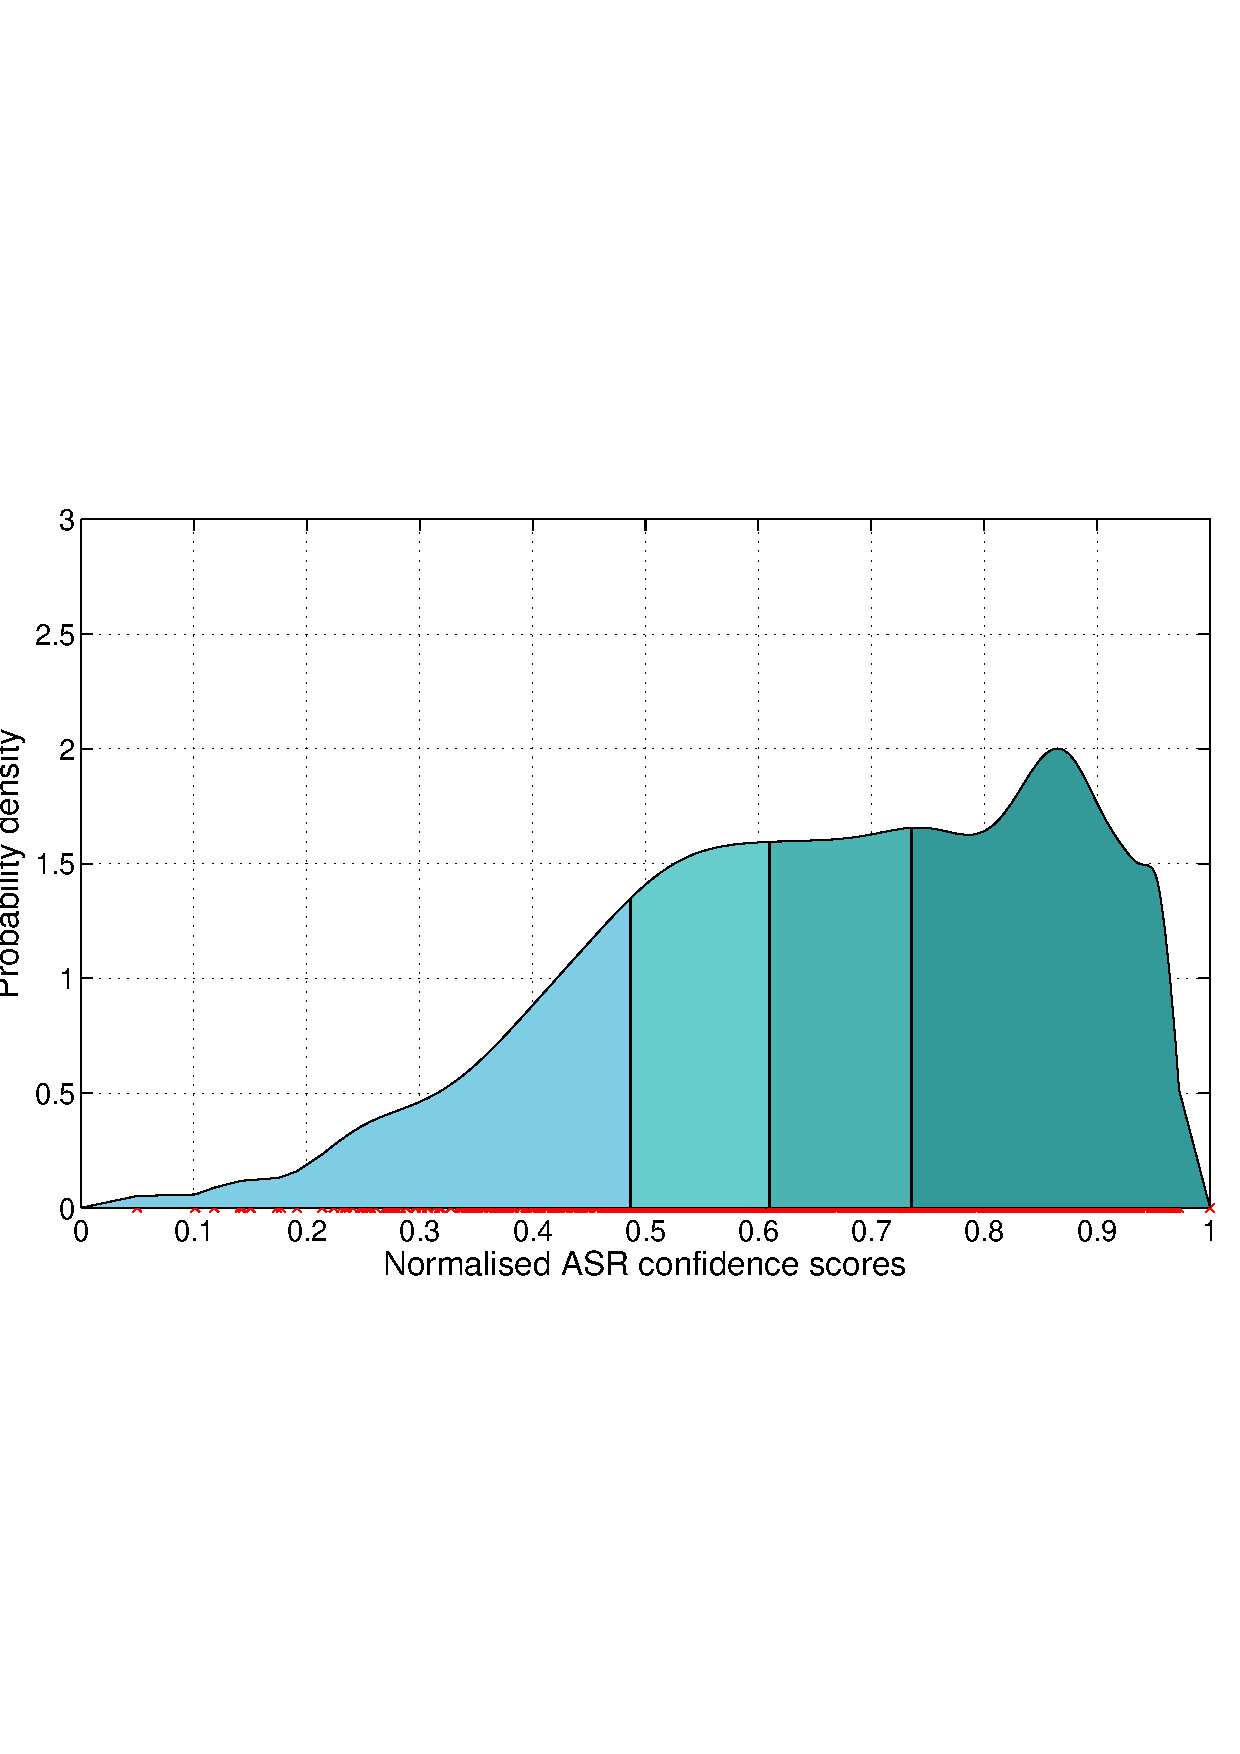
\includegraphics[scale=0.45]{imgs/asrconfidence.pdf} 
\caption{Probability density function for the probability values of the top hypothesis specified in the user dialogue act $a_u$, divided into four non-overlapping regions that respectively correspond to the first, second, third, and fourth+fifth quintiles of the distribution. The actual probability values are marked as red crosses on the X axis. }
\label{fig:asrconfidence-exp3}
\end{figure}


\subsection{Factored statistical model}

The second approach developed for this experiment consist of a traditional statistical model whose parameters are estimated from the Wizard-of-Oz data set collected for the experiment.  The parameter estimation is follows the Bayesian learning procedure presented in Chapter \ref{chap:wozlearning}. 

To reduce the problem of data sparsity, the model is factored in several smaller models. 

\subsection{Rule-structured model}

\subsection{Learning curves}

\section{User trials}

\subsection{Experimental setup}

\subsection{Metrics}


\note{various measures (number of turns, duration, number of disconfirm)}

\note{direct assessment of user satisfaction}

\subsection{Results}

\note{ANOVA, since we would have two baselines and our approach? (see e.g. Passonneau's article)}


\subsection{Analysis}

\section{Conclusion}




% note about our approach: generalisation enable a better account of the data sparsity problem.  plus, the state dynamics are not lost since we perform belief update.  Finally, the appraoch can be seen as an initial boostrapping that can then be further refined through online reinforcement learning (Bayesian prior), as in Williams etc. also, we learn utilities, not a direct classification. Also: a user simulator is difficult for situated and open-ended environments.  we learn a POMDP policy by simulation


\chapter{Concluding remarks}
\label{chap:conclusions}

\section{Summary of contributions}

\section{Future work}

\note{Formally characterise the expressivity of the rules and extend them to handle Ginzburg style update rules?}

\note{Try to learn a policy in a fully online fashion with real users, without simulator}

\note{do online reinforcement learning with real users and combine imitation+reinforcement learning}


\appendix

\chapter{Relevant probability distributions}
\label{chap:probdistributions}

\section*{Uniform distribution}

\section*{Multinomial \& categorical distribution}

\section*{Normal distribution}

\section*{Dirichlet distribution}

\section*{Kernel distribution}

\note{Should we include the last one?}

%
\chapter{Additional Proofs}
\note{chap:proofs}

\note{derivation of the MLE estimate for a categorical distribution by deriving the likelihood function.  Use Lagrange?}

\note{show that the posterior distribution after seeing an example is not a dirichlet anymore, but is still in the exponential family.  --> really useful?we are only dealing with partially observed data anyway}


\chapter{Domain specification for user trials}

\note{put here a summary of the probabilistic rules applied in the last experiment (user evaluation)}

\backmatter


\bibliography{lt-biblio}

%\newpage
%\phantomsection

%\printindex

\end{document}
